\documentclass[12pt, oneside]{extbook}

\usepackage{geometry}
\usepackage{graphicx}
\usepackage{listings}

\geometry{
	a4paper, 
	top = 2cm,
	left = 1.5cm,
	right = 1.5cm,
	bottom=2cm
}

\title{Sistemi Operativi Avanzati}

\begin{document}
\maketitle
\tableofcontents
\chapter{Hardware Insights}
\section{Introduzione - dettagli hardware}
Analisi di aspetti che riguardano come i processori sono fatti, come si comportano e come questo impatta sul software in esecuzione. Cominciamo già ad introdurre una serie di problemi per la parte di sicurezza.\\ L'IT si è evoluto dall'Assembly verso B/C, C++, Web API etc... Quindi, astrazioni sempre più lontane da ciò che accade in un sistema, più ci si allontana, più si perdono caratteristiche relative alla parte hardware ovvero dal capire cosa accade quando si scrive qualche applicazione. Si perde anche la capacità di configurazione e la capacità di sviluppare nuove cose, che si scontrano con l'hardware.\\ L'informazione che si perde spostandosi verso l'alto: lo stato del programma è un ecosistema di componenti hardware e software, quando si lavora ad alto livello e si guarda solo il framework specifico è perso. Inoltre, il software oltre a toccare le risorse presenti nell'ISA (registri, memoria etc...), tocca anche lo stato di risorse non nell'ISA\footnote{L'ISA è l'insieme di istruzioni che compongono il linguaggio macchina dello specifico calcolatore.} se ho un'istruzione che sposta il dato da un registro ad un altro, lo stato dell'hardware cambia non solo dei registri, ma anche in altro.\\ Ci sono dei footprint lasciati dal software in esecuzione sull'hardware che vanno conosciuti.\\\\ Ci sono sorgenti che, se astratte, si perdono:
\begin{itemize}
\item compiler decision: se non conosciamo le istruzioni usate, perdiamo i side effect
\item hardware run-time decision: tutti gli step che l'hardware esegue per portare avanti un program flow. Quando l'hw esegue le istruzioni, non le esegue sempre allo stesso modo, perché può cambiare lo stato interno. Una delle cose più interessanti è relativo all'hyper-threading: ho dell'hw, unico motore, quanti flussi di istruzioni eseguo? Con l'hyper-threading più di un flusso e quindi bisogna decidere come distribuire la capacità computazionale fra le varie istruzioni. \\ Inoltre, su hw moderno tutte le istruzioni sono eseguite in parallelo, una volta l'istruzione può essere eseguita con i dati in cache ed un'altra no: sono due situazioni differenti.
\item disponibilità o assenza delle risorse hardware
\end{itemize}
Ci piacerebbe capire il dettaglio di tutto.\\ Possiamo sfruttare soluzioni già scritte da altri, in quanto chi le ha scritte sapeva come farlo, ma è utile scendere nel dettaglio, inoltre non è detto che chi ha ideato le soluzioni lo abbiamo fatto scrivendole nella maniera più efficiente o corretta. Oggi, l'hardware è multi-core, e questo caratterizza alcuni aspetti importanti che vanno riflessi nella programmazione del software.
\subsection{Primo esempio: Bakery algorithm di Lamport}
Vediamo l'esempio del bakery algorithm proposto da Lamport per risolvere il problema dell'accesso condiviso in una sezione critica.
\begin{lstlisting}
var choosing: array[1,n] of boolean;
	number: array[1,n] of int;


var choosing: array[1,n] of boolean;
number: array[1,n] of int;
repeat {
	choosing[i] := TRUE;
	number [i] := <max in array number[] + 1>;
	choosing[i] := FALSE;
	for j = 1 to n do {
		while choosing[j] do no-op;
		while number[j] =/= and (number [j],j)< (number [i],i)
		do no-op;
	}
	<critical region>;
	number[i] := 0;
}until FALSE
\end{lstlisting}
posso avere concorrenza reale fra thread, oppure una concorrenza logica. Affrontiamo il problema della sezione critica, si entra a turni e sempre almeno uno è dentro.\\ Per sincronizzare i thread ci sono dei dati condivisi in memoria, due array.\\ Quando un thread vuole entrare, si alza un flag (ovvero si setta a true la propria entry di \textbf{choosing}), si sceglie un numero d'ordine (massimo letto +1) e poi si chiude il flag. Occorre aspettare poi il proprio turno, e questo avviene in due cicli consecutivi:
\begin{enumerate}
\item in un primo ciclo, si aspetta che tutti quanti gli altri abbiamo messo il loro flag a false
\item in un secondo ciclo, si verifica che sia il proprio turno, sia verificando che chi viene prima abbiamo rimesso a posto il numero e sia confrontando la propria coppia (numero, indice) con quella degli altri
\end{enumerate} L'attesa è attiva: è a livello utente, non c'è nessuna chiamata al SO, ed è basata sui numeri ed anche sugli ID dei processi. Facendo girare l'algoritmo sulla propria macchina, ci sono dei problemi dati dall'aver utilizzato un linguaggio come il C senza sapere quale sarà l'hw dove girerà il sw. \\ L'idea è quella di verificare, tramite logging, se il valore del token \textit{tokens\_to\_distribute} viene preso doppio o viene saltato qualche decremento.\\ Se si prova a far girare il codice in locale, si nota che il logging riporta un problema per il valore -3229289: difatti, due letture consecutive leggono questo stesso valore, mentre il secondo doveva essere -3229288.\\ Il motivo del non funzionamento sta nel fatto che nessuna macchina off the shelf è \textbf{sequentially consitence}. Quello che succede non è relativo alla compilazione, quindi va in esercizio un programma scorretto, ma l'hardware a run time fa delle cose che non conosco, quindi se questo non viene evitato non è possibile eseguire sw di sistema.\\ Quindi. cominciamo a muoverci per capire cosa accade in hw, ovvero le differenze fra un modello di hw ed il vero hw. Il modello di macchina a cui siamo abituati a pensare presenta le seguenti caratteristiche (macchina di von Newman):
\begin{itemize}
\item astrazione di una single CPU
\item astrazione di una single memory
\item single flow control abstraction fatto di fetch, execute e store
\item transizioni di stato nell'hw che sono separate nel tempo: c'è una sola istruzione in flight per ogni istante di tempo
\item immagine definita della memoria allo startup di ogni istruzione
\end{itemize}
Vedendo il processore così, è come se non si eseguisse in parallelo. L'approccio moderno di pensare l'architettura è differente, difatti si considera il concetto di \textbf{scheduling}, cercando di pianificare come fare le cose affinché quello che realmente si fa è \textit{equivalente} ad un program flow va a specificare che debba succedere.
\subsection{Scheduling e parallelismo}
Abbiamo quindi un program flow, ma non è più vero che quando viene eseguita una istruzione le precedenti hanno impresso l'output come side effect nell'hw, quello che si cerca di fare è mettere in scheduling l'istruzione come se tutto fosse sequenziale, ovvero come se si stesse eseguendo ciò che è dettato nell'execution flow.\\ Quando poi si astrae dall'hw, si recupera lo scheduling anche a livello sw: un conto è decidere cosa fare del flusso nell'engine, un conto è decidere quali dei molteplici flussi paralleli associare all'engine.\\ È possibile seguire una regola parallela, basta che il program flow non vada diversamente da quanto scritto nel software e quindi c'è la \textbf{propagation of values}, quindi il valore va propagato in avanti per istruzioni successive. 
Quindi, a livello hardware, lo scheduling definisce:
\begin{itemize}
\item l'esecuzione delle istruzioni all'interno di un singolo flusso di programma
\item l'esecuzione in parallelo (speculativa) di diversi program flows
\item la propagazione dei valori verso la memoria complessiva
\end{itemize}
A livello software invece, abbiamo:
\begin{itemize}
\item la definizione dei time frames per l'esecuzione dei threads sull'hw
\item quando si parla di sw, non si eseguono solo thread, altrimenti il sistema sarebbe sordo rispetto agli interrupt che sono task a tutti gli effetti, quindi serve la definizione dei time frames per servire l'interrupt. Questo non è banale: nel task management, questo ha portato all'evoluzione smodata nei kernel Linux.
\item Sincronizzazione livello software, ovvero quando i thread devono eseguire le istruzioni macchina in CPU
\end{itemize}A livello hardware, c'è \textbf{l'Instruction Level Parallelism} (ILP): in una finestra temporale in cui una istruzione ha prodotto output, è possibile farne entrare un'altra, ovvero la CPU è in grado di processare 2 o più istruzioni dello stesso flusso di esecuzione nello stesso ciclo di clock.\\ Processiamo più istruzioni insieme, che fanno cose differenti e questo fa si che ad ogni ciclo di clock è possibile completare una istruzione, anche se una singola istruzione richiede più cicli di clock per terminare,e quindi di completare prima l'esecuzione complessiva.\\ A livello software c'è il \textbf{Thread Level Parallelism: }ci possono essere più program flow che portano avanti la logica, quindi possiamo pensare il programma come la combinazione di molteplici flussi concorrenti.\\ Su un'architettura ILP non per forza siamo paralleli a livello di thread, ma vale invece il contrario per il parallelismo sw.\\\\ La velocità del processore spesso è misurata come Ghz, ovvero quanto impiega il ciclo di clock a cambiare stato.\\ Sappiamo però che una istruzione entra ad un certo ciclo di clock ed esce dopo un certo numero di cicli di clock, quindi può usarne un numero elevato, perché fa molte interazioni con l'hw o se ci sono delle asimmetrie o dei pattern di gestione dei dati. Quindi, parlando dei Ghz del processore non stiamo necessariamente parlando di quanto è veloce il processore, conta quali istruzioni usiamo e come queste sono combinate fra loro.\\ Un'altra cosa fondamentale riguarda le categorie di flussi di esecuzione:
\begin{itemize}
\item CPU bound: programma o thread che usa tutto il tempo di CPU a disposizione
\item I/O bound: chiama un servizio bloccante del kernel e quindi usa meno tempo di CPU
\end{itemize}
Esiste una ulteriore categoria di applicazioni, ovvero le \textbf{memory bound:} similari alle CPU bound, ma mentre il program flow del thread è in esercizio, molte delle istruzioni interagiscono con la memoria. Quindi, le istruzioni usano un alto numero di clock perché serve che arrivi qualcosa da qualche componente esterno verso il processore affinché continui l'esecuzione. Questo ha portato allo sviluppo dell'hw in modo da poter sempre fare lavoro utile anche se ci sono istruzioni bloccate nella CPU e quindi ad un ILP spinto a livello quasi estremi.\\ Alla luce di ciò, sono stati ri-progettati diversi processori, ma il problema scaturito è che l'accelerazione dei processori ha creato un gap fra velocità di memoria e velocità dei processori, che affligge le architetture moderne.
\subsection{Pipeline}
Una pipeline è il modo basilare di fare ILP, in quanto c'è overlap in processing di più istruzioni. La tecnica è hardware-based ed unisce lo scheduling ed il parallelismo: una istruzione inizia, e mentre questa fa qualcosa ce n'è un'altra che fa qualcos'altro, ovvero esegue delle istruzioni che richiedono di interagire con dei componenti differenti. C'è anche lo scheduling nella pipeline: quello che è scritto nel programma eseguibile non è necessariamente eseguito secondo la stessa sequenza nell hardware. C'è parallelismo, ma la sequenza delle istruzioni di un program flow non è eseguita necessariamente secondo la stessa sequenza del programma. Bisogna ovviamente mantenere la \textbf{causalità}, altrimenti l'architettura hw non può portare avanti il program flow in maniera corretta. Quindi, il modello di riferimento alla base della costruzione di tutte le architetture moderne è un data flow model, con il vincolo della causalità (nel flusso di programma): ogni istruzione che vediamo in realtà sta avvenendo in parallelo con molte altre, sia in lettura che in scrittura.\\ In una architettura pipeline semplice, una istruzione passa per fasi differenti ed usa nelle differenti fasi componenti diverse del processore, supponiamo di avere 5 stadi diversi per cui ogni istruzione deve passare:
\begin{itemize}
\item IF - Instruction Fetch
\item ID - Instruction Decode
\item LO - Load Operands
\item EX - Execute
\item WB - Write Back
\end{itemize}
La figura sottostante mostra un caso di esecuzione senza pipelining:
\begin{figure}[ht!]
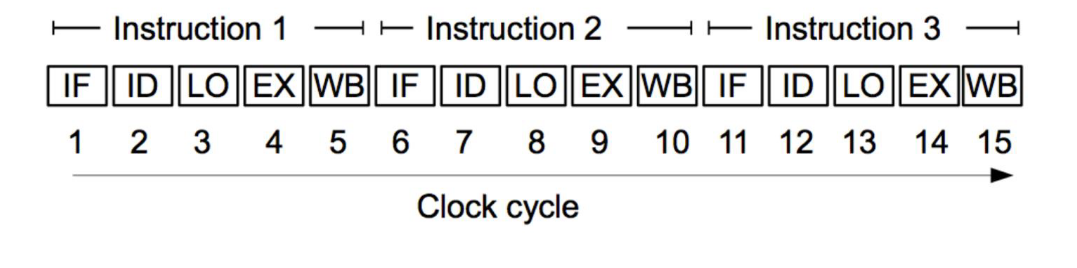
\includegraphics[scale=0.3]{immagini/no-pipeline}
\caption{Istruzioni senza pipeline}
\end{figure}
L'esecuzione in pipeline si basa sulla possibilità di sovrapporre le istruzioni, perché una istruzione non sta usando alcuni componenti della CPU che possono essere usate da altre: ad esempio, se una istruzione è nella fase di ID, di sicuro non starà usando i componenti necessari alla IF, e così valore per un'altra che è nella fase di LO o di EX. La figura in seguito mostra un caso di esecuzione con pipelining 
\begin{figure}[ht!]
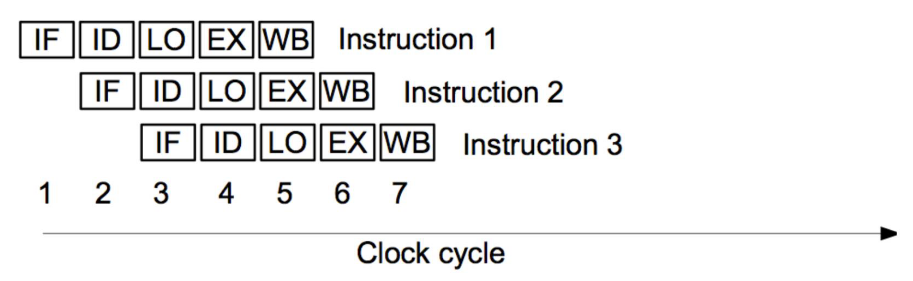
\includegraphics[scale=0.3]{immagini/pipeline}
\caption{Istruzioni con pipeline}
\end{figure}
Questo è l'ILP, e questo tipo di architettura è la base che, con altre tecniche, permettono di eseguire altro per affrontare problemi come il fatto che ogni operazione come la LO richieda più cicli di clock. Non sappiamo a priori quanti cicli di clock richiede una istruzione, quindi il problema va affrontato. Inoltre, l'altro problema è legato ai \textbf{breaks:}se ho un'istruzione di salto e riesco a capire dove saltare solo quando l'istruzione è finalizzata, l'istruzione che viene inserita in seguito a questa potrebbe essere differente da quella da immettere effettivamente e che si saprebbe solo alla fine. Questo è il problema può essere di due tipi:
\begin{itemize}
\item \textbf{control dependency};
\item \textbf{data dependecy}, dove il dato è richiesto da una istruzione in un momento in cui non è disponibile.
\end{itemize} 
\textbf{esempio: analisi di speedup}\\
Supponiamo di voler fornire N risultati, uno per ogni istruzione e di avere L stadi di processamento ed un ciclo di clock di lunghezza T.\\ Senza pipeline, avremo un delay pari a \[ N \cdot L \cdot T\]. Con il pipelining, otteniamo un delay pari a \[(N+L)\cdot T\] dove lo speedup sarebbe dato da \[\frac{N \cdot L}{N+L}\], ovvero circa L per un N grande.\\ Ovviamente, maggiore è L e più il fattore di speedup cresce, ma tipicamente i processori pipelined hanno sui 10 stadi massimo.\\ Ovviamente, abbiamo uno speed up ideale, il problema è che non consideriamo i problemi sopra citati: non è detto che si riesce a committare una istruzione per ogni ciclo di clock, quindi possono essere richiesti molti più cicli di clock. Ampliando la pipeline, si amplia la \textbf{capacità di fare}, quindi inserire nel processore hw per fare operazioni che poi magari non vengono eseguite.
\subsection{Processori moderni}
Gli stage di pipeline non sono molti (ordine delle decine), quindi vediamo cosa è stato adottato per risolvere tutta la serie di problemi visti.\\ Abbiamo, fra le soluzioni possibili:
\begin{itemize}
\item software stall: inseriamo, in un flusso di programma, delle istruzioni di stallo fra due istruzioni. Se ho un salto e non so dove, metto degli stalli finché so se saltare o meno; questo meccanismo è adottato dai compilatori
\item software re-sequencing (o scheduling): anche questo viene fatto dai compilatori, quando si rendono conto che c'è un blocco atomico di programma (ovvero un flusso eseguito nel complesso) si ri-organizza il blocco di istruzioni in modo che istruzioni che si dipendono siano più distanziate
\item per i salti, c'è la branch prediction: se non si sa quale è l'istruzione a cui saltare, si fa una previsione e si fa il fetch di quella zona di codice predetta
\item \textbf{out-of-order pipeline (OOO)}: la base di ciò che accade in una architettura moderna. Importantissimo per permettere alla CPU di essere efficace ed efficiente con generiche sequenze di istruzioni: se una istruzione deve aspettare dei dati, un'altra successiva può andare avanti superandola fino anche completare, \textbf{ma senza rendere visibili le cose nell'ISA}, o si violerebbe il flusso di programma. Quindi, l'OOO non è basato su come le istruzioni toccano l'ISA, ma sul fatto che alcune istruzioni devono aspettare e quindi è possibile far passare avanti a queste le altre.
\end{itemize}
\section{La pipeline nell'x86}
Il processore x86 a 64 bit moderno ha più o meno lo stesso set di registri di un processore di un processore come l'8086 (ed altri), la differenza è che sono un po' di più e sono più grandi.\\ I cambiamenti sono interni, ovvero nel come vengono eseguite le istruzioni: i486 è stato il primo ad adottare una architettura pipeline, che viene riportata in seguito
\begin{figure}[ht!]
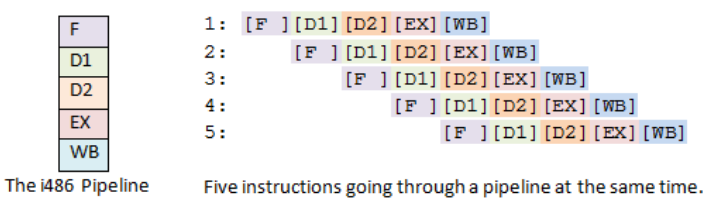
\includegraphics[scale=0.4]{immagini/pipeline-i486}
\caption{Pipeline di i468}
\end{figure}
L'architettura non è "piaciuta" molto, ad esempio se si esegue lo lo XOR fra due registri e si fa per 3 volte consecutive, ognuna delle istruzioni dipende dal risultato precedente in quanto ha una sorgente coincidente con la destinazione, e questo rallentava tutta la pipeline.\\ Se ad esempio, consideriamo del codice C che accede ad un puntatore ed in un caso accede e poi incrementa il puntatore e nell'altro caso accede dopo aver incrementato, questo ha un effetto totalmente diverso. È possibile sperimentare lo stesso problema anche in linguaggi di più alto livello, ad esempio se si incrementa un puntatore:
\begin{itemize}
\item a = *++p
\item a = *p++
\end{itemize}
c'è una differenza in performance evidente fra i due statement. Il file \textit{PIPELINE-TEST/backward-propagation.c}, che gira per 20000 iterazioni, permette di specificare con una macro di compilazione DEPENDENCY se:
\begin{itemize}
\item accedere al puntatore dopo averlo incrementato (e quindi dover dipendere dall'istruzione precedente
\item oppure, se disabilitato, accedere e poi incrementare il puntatore
\end{itemize} 
Se si esegue il programma, si ottengono i seguenti tempi (dipendenti dalla macchina di esecuzione):
\begin{itemize}
\item con dipendenza, si ottiene un tempo di 5.25 secondi
\item senza invece, il tempo è di 5.31 secondi
\end{itemize}
C'è inoltre il problema di istruzioni che causano lo squash della pipeline, ovvero la cancellazione di tutto ciò che vi è contenuto in quel momento. Tali istruzioni possono essere denotate come danno nel nostro programma, in quanto è possibile che vada rifatto tutto il lavoro perso delle successive istruzioni. Se consideriamo x86, una istruzione di questo tipo è \textsf{CPUID}, che prende l'ID numerico del processore su cui si sta lavorando. Questo è fondamentale quando si scrive del sw per il kernel, specialmente quando si sta scrivendo del sw che tocca delle strutture dati per lo specifico processore: bisogna conoscere quale è il processore su cui si lavora.\\ Tali istruzioni sono dette \textbf{serializing}, se però leggiamo il manuale dell'istruzione CPUID ci dice che è garantito che tutto ciò che viene è stato fatto da istruzioni precedenti è stato completato prima che la prossima istruzione sia fetchata ed eseguta.
\subsection{Intel x86 superscalar pipeline}
Per poter superare il problema degli effetti del sw all'interno dell'esecuzione in pipelining è necessario avere una  pipeline avanzata, in modo da poter capire cosa è possibile eseguire in parallelo: questo ha portato allo sviluppo delle \textbf{superscalar pipeline}.\\  Tale pipeline è fatta in modo che in ogni fase c'è più di un componente, ad esempio più componenti di esecuzione, più ALU, che possono essere identici e permettere quindi che l'istruzione possa andare in uno di essi. Se ad esempio l'istruzione richiede l'engine per più cicli di clock, non blocca successive istruzioni che magari poi richiedono lo stesso componente in quanto tale componente è ridondato. C'è quindi parallelismo nella pipepline stessa, inoltre siccome le istruzioni più lente, e che quindi richiedono più cicli di clock, sono un problema, i processori hanno adottato il modello dell'out-of-ordering: se qualche istruzione è ferma, le altre vanno avanti rispettando comunque il data flow model.\\ Tali aspetti erano nati molto prima, ad esempio nell'IBM 360/91 degli anni 60', si parlava però di architetture particolari ed il tutto preveda che nella pipeline ci fossero altri componenti per gestire l'OOO.\\ Le basi del progetto erano:
\begin{itemize}
\item come mettere in commit le istruzioni in program order: fare uscire una istruzione dalla pipe indica che l'effetto dell'istruzione sulle risorse dell'ISA divine visibile, quindi è delicato capire quando mandare in commit
\item processare istruzioni indipendenti, sia sui dati che sulle risorse, il prima possibile
\end{itemize}
Vediamo come affrontare il problema che ogni istruzione possa durare un certo numero di cicli di clock
\subsubsection{Istruction span problem}
Ogni istruzione può durare un certo numero di cicli di clock, a seconda di cosa deve fare e per effetti diversi, ad esempio può essere necessario attendere componenti esterni alla CPU come la memoria. Il fetch dei dati può portare via diversi cicli di clock, e si è cercato di risolvere questo come problema centrale con le pipeline super-scalari.\\ Con una OOO pipeline, può accadere la seguente cosa\\\\
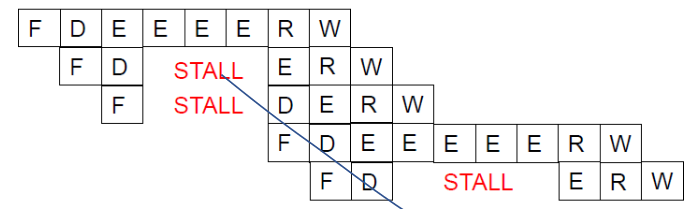
\includegraphics[scale=0.5]{immagini/ooo-pipeline-1}\\
la seconda istruzione può avere uno stallo, magari perché non ha i dati. Come vediamo, in realtà l'istruzione ha bisogno di un solo ciclo di clock di esecuzione, ma ne usa di più perché non ha i dati disponibili. Anche la 3° istruzione è bloccata e lo stesso vale per l'ultima, perché deve usare lo stesso componente. Ricordiamo che il delay può avvenire perché il componente da usare non è pronto.\\ In OOO accade la seguente cosa: lo stallo diviene un ri-ordinamento\\\\
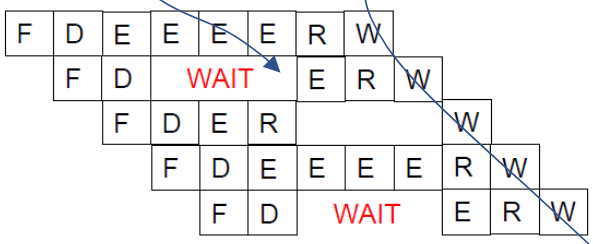
\includegraphics[scale=0.5]{immagini/ooo-pipeline-2}\\
può accadere che istruzione 1 e 2 usino due componenti identici nella pipeline, e che la 3° entri in esecuzione ed abbia pronto il risultato molti cicli di clock prima di quando serve, quindi occorre mantenerla uncommitted e metterla in write back solo in maniera coordinata. Ad ogni ciclo di clock è possibile mandare in commitment il lavoro anticipato: se riusciamo a far entrare una istruzione ogni ciclo di clock, riusciamo a farne uscire una ogni ciclo di clock, avendo lo stesso throughput in ingesso ed in uscita rispetto alla pipeline tradizionale.
\subsection{Pipeline OOO speculativa}
Quando si parla di pipeline OOO, si parla anche di pipeline speculative: su un flusso di programma, se processiamo una istruzione successiva rispetto ad una che deve ancora essere processata, stiamo dicendo che c'è indipendenza fra le due, ma questo non è sempre vero. Quello che è in pipeline sta in realtà eseguendo in maniera \textbf{speculativa}, si fa fetch di una istruzione successiva e poi magari le istruzioni non verranno eseguite perché si salta altrove. Inoltre, una istruzione in qualunque ciclo di clock può generare una \textbf{trap}: si potrebbe consultare il TLB (caching), ci rendiamo conto che qualcosa non va e quindi l'istruzione non può essere mandata in commit. Se c'è una trap mentre un program flow esegue, va passato il controllo ad un gestore lato sw, quindi tutte le istruzioni che venivano eseguite dopo erano eseguite in maniera speculativa e non andranno mai a commit point.\\ Distinguiamo fra due concetti:
\begin{itemize}
\item il \textbf{retire} è l'azione del committare una istruzione e rendere i suoi side effects "visibili" in termini di ISA;
\item l'\textbf{emissione} è l'azione di iniettare le istruzioni nella pipeline.
\end{itemize}
Fra le due azioni è possibile che ci siano altre istruzioni di mezzo, ci sono poi anche le eccezioni che vanno gestite correttamente: se una istruzione successiva entrata in pipeline e genera una eccezione, ha senso eseguire un cambio di flusso per gestire l'evento particolare? No, in quanto l'istruzione è eseguita in modo speculativo e quindi finché non arriva alla fase di write back può scomparire dal flusso, perché anche le istruzioni precedenti sono speculative e magari una istruzione precedente genera l'eccezione che rende l'eccezione di quella successiva inutile, perché l'istruzione non doveva proprio essere nel flusso di programma.\\ Quindi le eccezioni sono imprecise, non è detto che quando vengono generate queste esistano o meno, saranno effettive solo se le istruzioni arriveranno al commit point.\\ Inoltre, l'eccezione viene generata considerando che in parallelo stiamo facendo altro in una OOO pipeline:
\begin{itemize}
\item una istruzione precedente è stata superata
\item una istruzione successiva ha superato
\end{itemize}
quindi quando viene generata la trap, lo stato effettivo del processore e di conseguenza quello di tutti i componenti non esposti nell'ISA globalmente può essere stato cambiato in modo parziale da istruzioni che precedevano quella che ha generato la trap, ma anche da istruzioni successive. Quindi, come implicazione importante, tutte queste istruzioni possono generare dei side effect che possono essere sfruttati per attaccare le applicazioni ed i sistemi, prelevare dati a cui non si può accedere etc...\\ Di seguito, viene mostrato uno schema esemplificativo della pipeline OOO\\\\
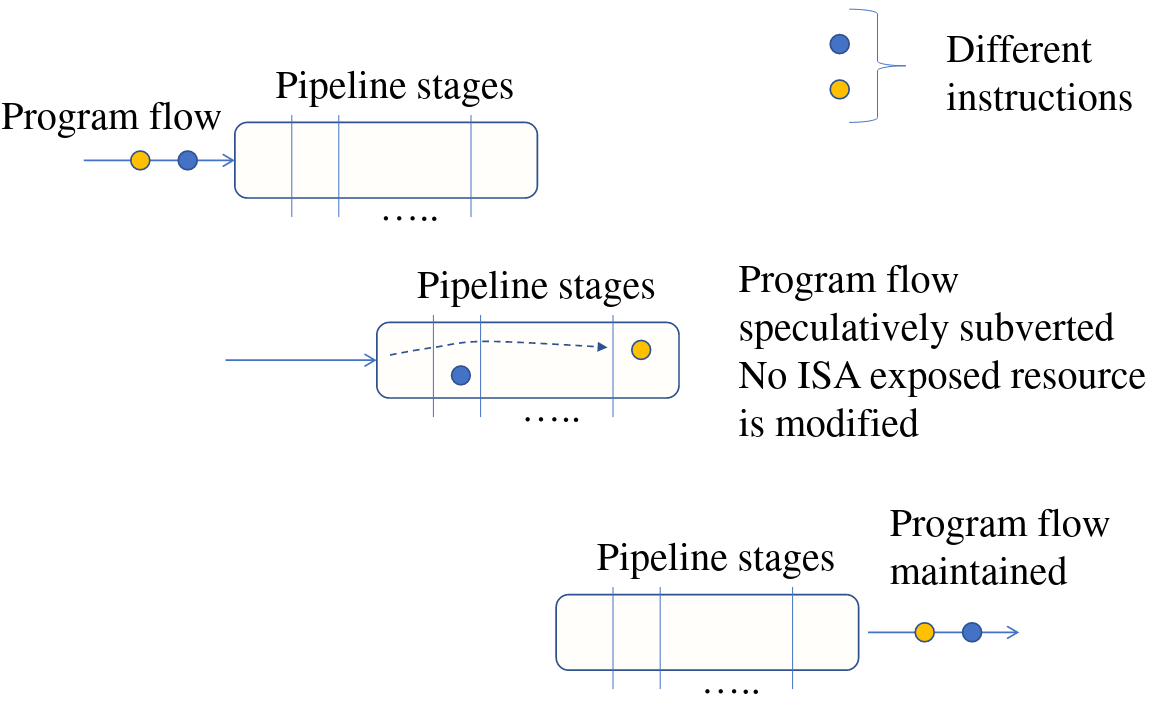
\includegraphics[scale=0.2]{immagini/pipeline-ooo}\\
come mostrato nell'esempio, può accadere che l'istruzione gialla arrivi a commit point prima  di quella blu e questo permette di portare a termine lavoro utile anche quando altre istruzioni sono bloccate per i vari motivi detti prima.
\subsubsection{Eccezioni imprecise}
Su una architettura pipeline OOO (ma anche generale) in cui le istruzioni si superano l'un l'altra con un ILP molto elevato, consideriamo che una istruzione A è dopo una B nel program flow e B che causa una eccezione. Quindi, B $\rightarrow$ A (B precede A) ed A entra in pipeline prima di B, ma se B ha una eccezione, possono esserci tante altre istruzioni successive che l'hanno superata dopo A in pipeline e queste possono aver cambiato molto nello stato della CPU, tutte le relazioni di dipendenza possono essere state portate avanti in maniera speculativa senza toccare i registri di CPU, ma toccando altri elementi. Può accadere che ci siano anche altre relazioni, ad esempio B genera dei valori che poi verranno usati da A e che A poi passi il risultato basato su tali valori ad altre istruzioni dopo di lei etc... \\ Si toccano componenti nella CPU in funzione del fatto che vengono anche passate informazioni in maniera speculativa e non a livello dell'ISA. Questa è stata la base dell'attacco \textbf{meltdown}, in cui è stata necessaria la patch di tutti i kernel esistenti: è possibile usare i processori OOO per leggere dati del kernel, è possibile leggere buffer cache e quindi leggere i file o i meta-dati per proteggere i dati (ad esempio dati di cifratura).
\\ Quindi, se siamo in pipeline occorre stare attenti, altrimenti si scrive software di sistema non corretto. Può accadere che viene passato un output in maniera speculativa e che ci siano effetti su altri componenti della CPU. \\ Considerando lo schema seguente:
\begin{figure}[!ht]
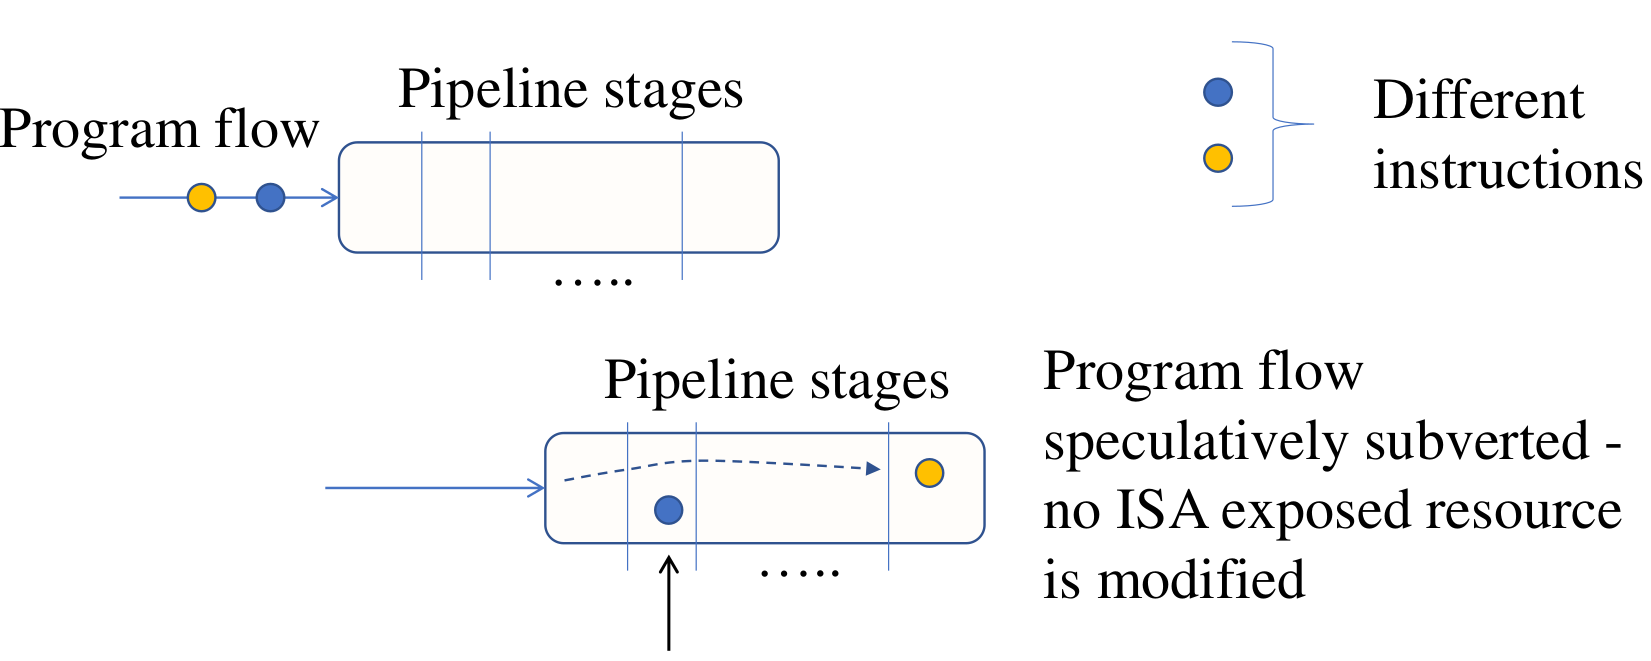
\includegraphics[scale=0.15]{immagini/not_valid_instr}
\end{figure}
Se l'istruzione accede a delle risorse non valide, come locazioni di memoria o componenti della CPU non accessibili temporaneamente, il flusso di programma non è più valido e quindi anche le altre istruzioni non sono valide, ma possono esserci dei side effect nell'hardware dovuti al fatto che tali istruzioni sono già state processate
\subsection{Algoritmo di Robert Tomaluso}
Le architetture moderne hanno delle varianti rispetto a questi algoritmi. Consideriamo come avviene il passaggio fra due istruzioni A e B per cui A$\rightarrow$B nel program flow, le possibili dipendenze sono:
\begin{itemize}
\item RAW (Read After Write): B legge un dato prima che A lo scriva, il che porta ad uno stallo e quindi c'è una dipendenza sui dati
\item WAW (Write After Write): B scrive un dato prima che A scriva lo stesso dato. Anche qui abbiamo una dipendenza sui dati
\item WAR (Write After Read): B scrive un dato prima che A legga lo stesso dato, quindi il dato letto non è consistente.
\end{itemize}
Come risolviamo queste dipendenze sui dati: Tomasulo propone delle idee algoritmiche per un processore OOO:
\begin{itemize}
\item RAW: per ciascuna lettura, bisogna tenere conto se il valore da leggere è già stato prodotto, l'attesa del dato va quindi inserita nella OOO e quindi nel caso sia necessario bisogna considerare il buffering dell'operazione;
\item WAR e WAW: la soluzione adottata è quella dei \textbf{renamed registers}. 
\subsubsection{Renamed registers}
Supponiamo di avere un registro R, per gestire WAW facciamo si che i due valori siano scritti ma sue due registri diversi. R non è un singolo registro, bensì è un \textbf{multi-registro}, dove ci sono varie versioni del dato. Qualsiasi istruzione che deve scrivere un valore in un registro ed entra in pipeline va sul componente, preleva uno slot utilizzabile fra i molti che compongono il multi-registro e scrive il valore in quello slot. Quindi, nel program flow può accadere che i valori possono essere scritti in tempi differenti sullo stesso registro, ma grazie alla presenza degli slot si risolve WAW, in quanto in termini di commit del valore verrà ristabilito l'ordine corretto. Il valore non può sovrascrivere, perché viene scritto su uno slot, quando viene mandata in commit l'istruzione si avrà il valore effettivo associato al registro R, nel controller del registro c'è anche quale è la versione attuale del valore del registro.\\ Un solo valore alla volta è quello attivo, alcune versioni saranno del passato ed altre del futuro, nella storia dei commit che poi verrà realizzata.\\\\
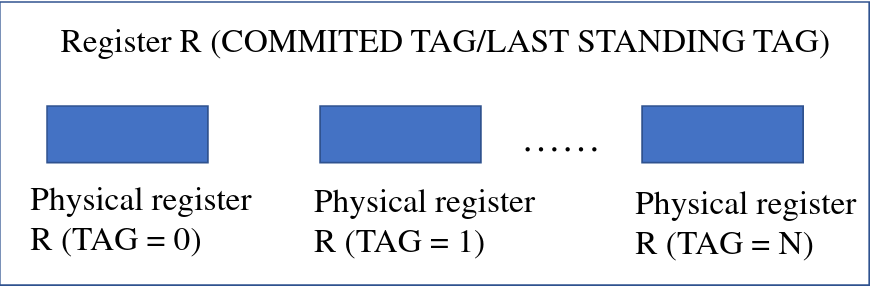
\includegraphics[scale=0.25]{immagini/multi-registri}\\
Quindi, quando mandiamo in pipeline una istruzione che deve leggere R, la marchiamo con il valore che quella deve leggere e finché il registro non è pronto l'istruzione rimane bloccata. Tutto questo è invisibile al programmatore in termini di risorsa ISA, ma visibile in termini del fatto che è possibile far si che il software faccia cambiare stato a tutti i registri in modo da creare problematiche.\\ In maniera indiretta è stato risolto anche WAR: per WAW è stato risolto il problema utilizzando i tag, ma anche per WAR finché il tag da leggere non è pronto, l'istruzione rimane ferma
\end{itemize}
\subsubsection{Reservation stations}
Ogni istruzione ha un codice operativo, che va bufferizzato da qualche parte e poi va relazionato al componente che deve eseguire l'operazione. La reservation station è una zona del processore che svolge tale funzionalità di buffer, in cui viene registrata una operazione in input all'oggetto (elemento operativo dell'hardware) che può eseguire quella operazione, ad esempio somme etc...\\  Non è detto che l'operazione venga processata immediatamente, perché può essere coinvolta in una dipendenza e dover attendere dei dati non ancora prodotti, questo viene dettato dallo stato del renamed register. La reservation station permette la possibilità di riservare il componente per l'istruzione, finché quest'ultima non è pronta ad essere eseguita.\\ Le reseravtion stations contengono:
\begin{itemize}
\item OP - l'operazione da eseguire (ovvero il codice);
\item $Q_j, Q_k$ - le reservation stations che produrranno l'input necessario ad OP;
\item in alternativa a $Q_j, Q_k$ ci sono $V_j, V_k$ ovvero i valori attuali (ad esempio i valori di registro) da usare come input per OPs
\end{itemize}
I registri, d'altra parte, sono marcati con la reservation station Q tale che produrrà il nuovo valore da scrivervi, se ce n'è bisogno.
\subsubsection{CDB e ROB}
Supponiamo di avere una reservation station in cui ci sia una operazione in coda: il flusso di informazioni fra le componenti deve essere supportato, che avviene usando il \textbf{Common Data Bus}, che permette di spostarle fra i vari componenti per garantire il corretto flusso di input fra le varie istruzioni.\\ Il \textbf{ReOrder Buffer} mantiene invece i meta-dati delle istruzioni non ancora committate, in quanto bisogna ricordarsi quale è l'ordine logico con cui andarle a committare, e questo tiene conto dell'ordine. Inoltre il ROB acquisisce tutti i nuovi valori prodotti dalle istruzioni (anche quelli che transitano nel CDB), mantenendoli uncommitted fino a che l'istruzione non viene ritirata. Questo mantenimento può essere fatto direttamente oppure referenziando l'alias di registro che deve mantenere tale valore.\\ Il ROB è anche usato per gli input delle istruzioni che necessitano di leggere valori non committati.
\subsubsection{Schema architetturale}
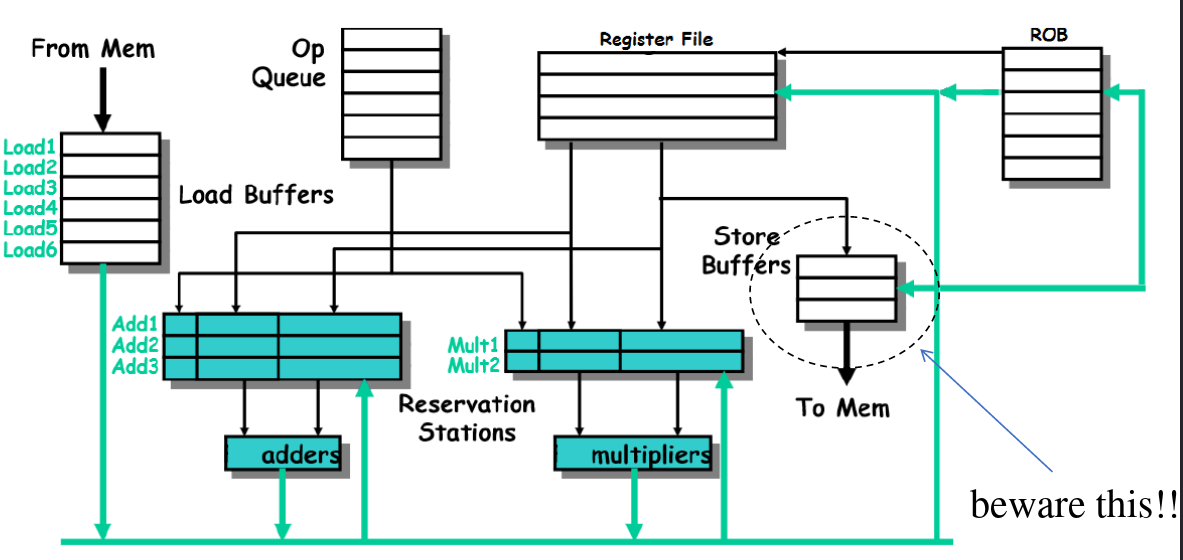
\includegraphics[scale=0.25]{immagini/arch-moderna}\\
Lo store buffer è un altro componente interessante: è fondamentale per interagire con la memoria. Mantiene in maniera temporanea il valore da scrivere per i dati verso la memoria. Lo SB viene toccato solo quando viene committata una istruzione, ed il valore viene scritto nello SB, non in memoria: in una architettura OOO quindi non si ottimizza solo il pipelining, ma anche la scrittura verso la memoria, perché se dovessimo scrivere in memoria a commit-time, la entry del ROB sarebbe occupata per vari cicli di clock e verrebbero bloccati diversi componenti senza poter andare avanti. Dallo SB i valori possono anche essere letti, e finché il valore non viene riportano in memoria è visto solo dal singolo program flow, magari perché questo necessita di ri-accedervi diverse volte durante l'esecuzione. Da qui scaturisce il problema della sequential consistency, dove se qualcuno produce qualcosa questo non è visibile ad altri.\\\\ \textbf{esempio:} abbiamo 3 istruzioni che entrano in pipeline, con i rispettivi delay $\delta$ per essere processate.
\\\\
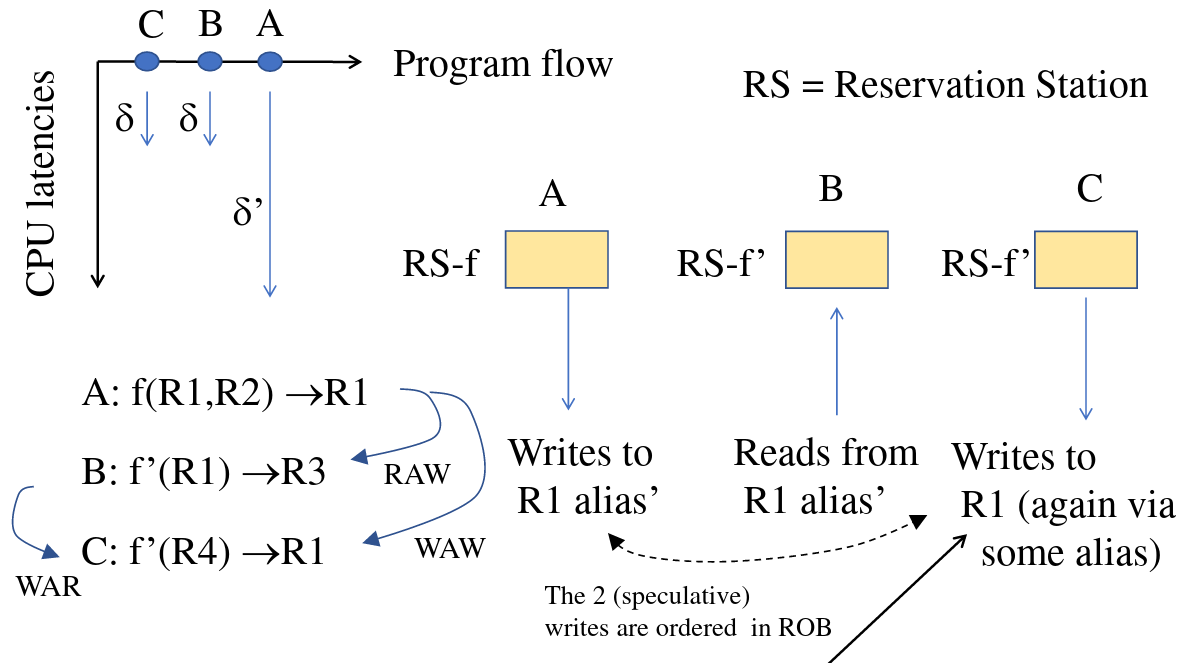
\includegraphics[scale=0.25]{immagini/ex-pipeline}
\newpage
Di seguito invece, viene mostrato un esempio che lega il ROB all'esecuzione delle istruzioni\\
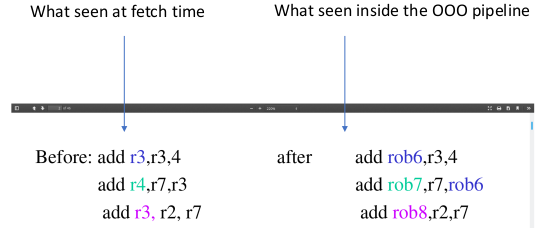
\includegraphics[scale=0.6]{immagini/rob}
\subsubsection{Storia}
Nell'architettura basata sull'algoritmo di Tomasulo, storicamente, venivano mandate out of order solo determinate istruzioni, mentre nei processori moderni l'OOO è visibile su tutto l'insieme delle istruzioni. Nell'evoluzione storica c'erano solo istruzioni in floating point, oggi si copre tutto il set di istruzioni
\subsection{Ancora sul memory wall}
Nel tempo, la memoria ha accelerato nella capacità di fornire informazioni, ma i processori hanno accelerato ancora di più nella richiesta delle chiamate a memoria. Quindi, guardando le 3 istruzioni precedenti ed i delay, ci sono anche i delay dovuti alla latenza per i miss in cache. Come vedremo, questo è stato il motivo della nascita delle architetture hyper-threading, ovvero la divergenza fra i due mondi.
\subsection{OOO nell'x86}
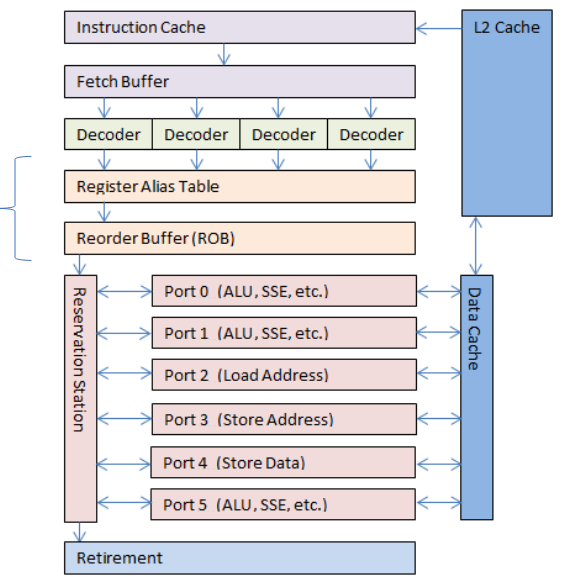
\includegraphics[scale=0.3]{immagini/x86-ooo}\\\\
A livello alto, nell'x86 abbiamo la Register Alias Table, il Reorder Buffer e tutta una serie di hardware replicato. Quando un oggetto entra nel Reorded Buffer, il firmware sceglie uno o l'altro componente replicato e ci sono poi le diverse relazioni che esistono fra i diversi componenti.\\ Questo fa capire che vengono caricate più le istruzioni alla volta, difatti viene caricata una intera linea di cache che in x86 è da 64 byte, in cui si possono mettere diverse istruzioni: alcune andranno in commit ed altre no, però ci sono molte cose che si passano informazioni e fanno attività.\\ L'OOO ha permesso di fare le operazioni talmente tanto velocemente che il core engine non veniva usato a pieno, anche per colpa delle latenze dovute agli accessi in memoria. Quindi, la questione posta fu quella di utilizzare lo stesso engine per molteplici flussi di programma, ovvero si introdusse \textbf{l'hyper-threading}, esposto al programmatore ad ogni livello, sia user che OS etc...\\ I registri esposti dall'ISA sono replicati, come se ci fossero due processori distinti, ma nel complesso l'OOO non viene esposto al programmatore, anche se il modo di scrivere il software può impattare l'efficacia dell'OOO stesso e, più in generale, il pipelining.
\subsubsection{Hyper-threading}
La necessità della nascita delle architetture hyper-threading è nata perché la struttura della CPU era talmente ottimizzata da rimanere senza fare nulla per troppo tempo, non riusciva più ad essere fillato in maniera efficiente quando i dati dovevano salire in memoria.\\ Le architetture ad hyper-thread prevedono che, siccome il "motore" è così rapido ed efficiente, si mandano due linee di input in parallelo, che sono due processori effettivi su un unico core: due program flow diversi su i due processori. Quando poi le istruzioni sono processate, si usa l'unico engine: il classico è avere 2-1 (es: 8 thread, 4 core). C'è una buona replicazione dei componenti, per evitare che se un flusso insista su un componente in particolare, non ci sia blocco.\\ Un altro aspetto importante è la sicurezza: se c'è un interferenza fra i due thread in esecuzione che prevede che si vedano dati di uno dall'altro, bisogna "spegnere" uno dei due e sfruttare meno potenza effettiva.
\\\\
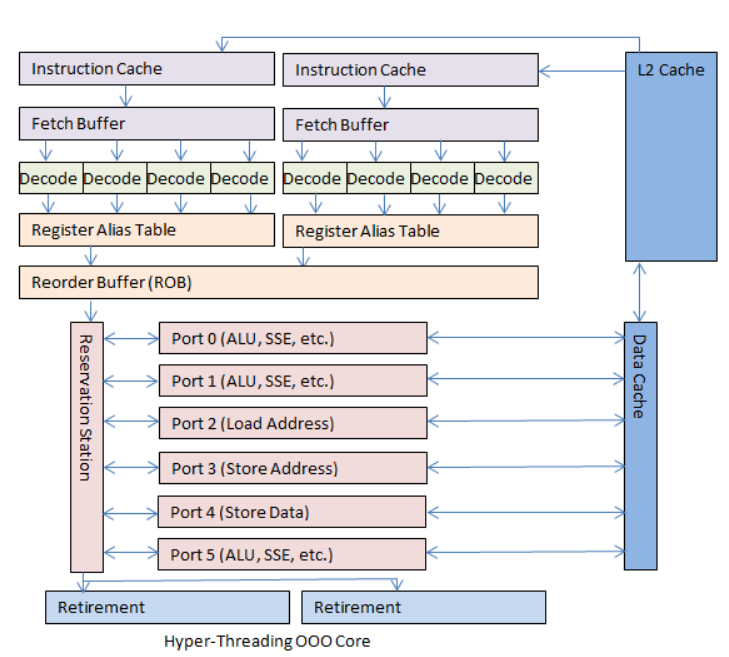
\includegraphics[scale=0.3]{immagini/hypert-ooo}\\
In questa architettura ci sono due hyper-thread ed una sola architettura per processare le istruzioni dei flussi e non c'è interferenza fra i due flussi, quindi quando l'istruzione scrive su un registro la risorsa è accessibile solo da quel flusso, ma la scrittura è tale per cui i componenti siano utilizzati per le istruzioni anche dell'altro flusso ma queste vengono usate in time sharing: gli oggetti non sono esposti nell'ISA, quindi questo non crea problemi a cosa è scritto nei programmi. In ogni caso, ci sono dei side effects sugli engine quando si esegue in hyper-threading, che sono problematici per la sicurezza.
\subsection{Gestione degli interrupt}
Ogni sistema moderno è interrupt-driven, quando c'è un interrupt bisogna eseguire una porzione di codice per rispondere agli interrupt.\\ Quando siamo sulla pipeline, avere un interrupt significa dire che siamo entrati con una serie di istruzioni sul thread corrente e l'interrupt vuole che si passi a prelevare istruzioni da un'altra zona di memoria, l'interrupt si accetta sempre quando una istruzione ha completato (per evitare di dover salvare lo stato dell'istruzione corrente). Per le altre istruzioni, che magari hanno già eseguito in maniera speculativa: 
\begin{itemize}
\item o si salva lo stato della pipeline;
\item oppure (più comodo) viene fatto lo squash della pipeline e si comincia a ri-fillare con le nuove istruzioni la pipeline
\end{itemize}
Questo ci fa capire che nei processori moderni l'interrupt costa: si butta del lavoro fatto e quasi finalizzato perché va squashato il contenuto nella pipeline, e quindi anche i valori scritti speculativamente negli alias dei registri, teniamo però bene in mente che le istruzioni in esecuzione e non completate e che vengono squashate possono aver cambiato lo stato micro-architetturale della macchina.\\ Ci saranno delle policy per distribuire questa cosa su tutti i core presenti nell'architettura.
\subsection{Trap e stadi della pipeline}
La trap è qualcosa di sincrono rispetto all'interrupt che è asincrono, capita perché il programma sta facendo qualcosa. Su una architettura pipeline, possono essere generate le seguenti trap in generali:
\begin{itemize}
\item Instruction Fetch \& Memory stages: l'istruzione può essere offending, quindi non è possibile finalizzarla per via di:
\begin{itemize}
\item Page fault, ovvero l'indirizzo di memoria logico a cui accediamo non sappiamo a cosa corrisponda;
\item Accesso in memoria misaligned, ovvero ci sono istruzioni che per lavorare correttamente hanno bisogno di indirizzi di memoria allineate ad una certa potenza di 2. 
\item Memory-protection violation, ad esempio scrivere su una pagina read only: tale informazione viene data dalla page table e cachata nel TLB
\end{itemize}
\item Instruction decode stage: operazione illegale, un program counter ha detto lungo un program flow di prelevare l'istruzione ed eseguirla nel processore ma questa non è eseguibile dal processore. 
\item Execution stage: possono esserci problemi sull'esecuzione vera e propria, ad esempio divisione per 0, quindi eccezioni aritmetiche
\item Write back: non ci sono eccezioni tipicamente
\end{itemize}
Per una certa istruzione, è possibile subito accorgersi se questa sia offending e quando viene identificata come tale, nel momento in cui entra in pipeline e non l'ha ancora attraversata, cosa si fa? Si butta tutto il lavoro in pipeline? No, perché questa potrebbe aver superato altre istruzioni e quindi sta eseguendo in maniera speculativa, per cui si rischierebbe di buttare cose che vanno finalizzate. Come ci si comporta: si può far cambiare il flusso all'interno della pipeline, eseguendo attività differenti nel momento in cui l'istruzione non fosse offending ed altre attività se lo fosse.\\ Oppure è meglio marcarla con un bit ad 1, in modo da ricordarsi che è offending e quando arriva a commit point, la mando in abort e possono mandare in abort tutto il resto perché a quel punto tutto quello che era precedente è andato in commit.\\ Perché la scelta migliore è la 2, ed è stata applicata nell'architettura di processore: quando un'istruzione attraversa una pipeline, viene gestita da un micro-codice, ovvero un sotto-sistema di controllo che sa cosa fare per ogni tipo di istruzione. Per gestirla in maniera adeguata, dovrei avere un micro-codice apposito per gestire una istruzione offending in un certo punto, quindi questo comporterebbe una complessità maggiore nel micro-codice per la gestione delle istruzioni. Quindi si evitano transistor per introdurre ulteriore logica, risparmiando spazio per ampliare l'hardware per fare delle operazioni più utili.\\ Quindi si aggiunge un bit ad 1 per indicare che l'istruzione è offending, ma questo vuol dire che tutti gli altri passi dell'istruzione vengono portati avanti: tutto quello che si fa per quella istruzione è tale per cui tutto quello che l'istruzione sta facendo non era permesso. Ma se ho un memory access violation, l'istruzione nella pipeline può aver passato in un alias di registro le informazioni lette nel caso della violazione e può essere letta da una istruzione successiva, questo crea una serie di side effect: A accede a dei dati non permessi, li passa a B ed etc... i side effects generabili sono funzione dei dati acceduti e questo è un problema.\\ Questo è l'attacco meltdown
\subsection{Meltdown attack}
Supponiamo di avere a disposizione un flusso di istruzioni in esecuzione in un'area di memoria, dove abbiamo un array di 256 byte. Supponiamo di avere un byte in un altra locazione di memoria: possiamo scrivere un programma che usa questo byte come offset nell'array (essendo 256 possibili valori, riusciamo ad indicizzare tutto l'array), accedendo quindi ad I[c]. Cosa è successo nell'architettura quando facciamo I[c]: abbiamo caricato c in memoria nel registro R ed usato R per accedere ad I. L'operazione di caricare c nel registro è in una architettura vera:
\begin{itemize}
\item può essere un'operazione speculativa, così come l'accesso in memoria usando il valore caricato di c
\item nell'architettura quello che accade e che un'istruzione ha chiesto di prendere c e metterlo in un registro. C'è un RAM per farlo fluire in un registro, c deve salire nell'architettura e passare per la cache. Quindi la lettura di c da usare come indice fa si che c passi comunque per la cache in una architettura moderna. Anche I[c] passa per la cache, se qualche istruzione vuole leggere questo byte deve passare anche lui per la cache.
\end{itemize}
Magari le due istruzioni sono offending, magari c è un valore inaccessibile al flusso di programma che è user-level e c è in zona kernel. L'istruzione va comunque avanti, con anche quelle successive, ma la cache ha cambiato stato. Quello che ha cambiato stato della cache è il fatto che uno dei caratteri è salito in cache, l'array potrebbe essere lecito perché magari è applicativo ed il che vuol dire che è stato creato un side effect per cui un suo byte è stato caricato in cache. Si può ri-accedere all'array dopo aver eseguito questa istruzione? Si, eseguendo una funzione di gestione del segmentation fault e posso capire se dato un array di valori alcuni sono in cache ed altri no: basta leggerli e misurare il tempo di accesso al valore per distinguere fra cache hit ed cache miss. Quello in cache sarà esattamente in posizione c e quindi posso dedurre il valore di c, che può essere un byte kernel sapce che non avrei dovuto leggere.\\ Riassumendo il funzionamento di meltdown:
\begin{enumerate}
\item facendo cache flush, fattibile a livello user. Possiamo limitarlo anche solo all'array desiderato
\item leggiamo un byte B di livello kernel
\item usiamo il byte B per leggere una zona di memoria lecita, quindi in questo caso l'array detto prima
\item L'istruzione intermedia è offending, la zona successiva è phantom perché non esisterà in quanto non andrà in commit, ma possiamo vedere se ci sono stati dei side effects.
\end{enumerate} 
L'array della cache non è di caratteri, ma è di pagine: una cache line porta vari byte, un minimo di 64 su x86 ma anche il doppio o il triplo, quindi se leggo un byte l'architettura ne porta in cache parecchi di più. Quindi il byte non va bene come unità di misura, non possiamo discriminare quale è il valore di c da inferire.\\ Le pagine sono di 4096 byte, e sono 256 pagine, usiamo c per accedere al 0-esimo byte della pagina, per cui c identifica la pagina a cui ho acceduto. Se la pagina non è in cache assolutamente, non era in cache, se invece il byte 0 c'è ed è seguito da altri allora c identifica la pagina.\\ Nella demo ci sono due comandi cat del file /proc/nome\_file perché così facendo, chiedendo al kernel il dato e scrivendolo altrove, i cat portano in cache i dati del segreto che sto cercando di scoprire e quindi velocizzano nell'operazione di retrieve che si cerca di eseguire.
\paragraph{Side channel:}per portare a termine il meltdown, si usa un side channel. All'interno dell'esecuzione è possibile generare dei cambi di stato che non sono visibili nell'ISA, perché non esistono istruzioni per leggere il dato direttamente dalla cache, ma che possono essere osservati in altro modo. Alla base di tutti gli attacchi su macchine moderne ci sono i side channel
\subsection{Dettagli di x86 64 bit - Instruction Set}
In x86 ci sono 16 registri general purpose a 64 bit, ma è retro compatibile con la versione a 32 bit in cui c'erano solo 8 registri a 32 bit.\\ I registri originali a 32 bit avevano determinati nomi ed è possibile utilizzarli ancora mediante il nome, per prendere i 32 bit meno significati del registro. Anche in un registro a 32 bit si possono gestire la metà del registro ed il singolo byte, lavorando a grana più fine, stesso vale per l'instruction pointer.\\ Ci sono poi altri registri per processare delle istruzioni particolari, che sono a 128 bit e poi dei registri per le istruzioni floating point.\\ Le istruzioni sono abbastanza e semplici similari:
\begin{itemize}
\item \textsf{mov\{b, w, l\}} (se byte, word o longword) \textsf{source dest}. Se non si specifica la size, la mov lavora a 64 byte
\item \textsf{push\{w, l\} source}
\item \textsf{pop\{w, l\} dest}
\end{itemize}
Per costruire un indirizzo per accedere alla memoria si può fare o con un indirizzo assoluto oppure specificando un offset all'interno dell'address space. In generale un indirizzo su x86 può essere targato con
\begin{itemize}
\item displacement, a questo possono essere sommati altri punti
\item base: può contenere un puntatore per accedere alla memoria
\item index + scale: altro offset che si può aggiungere ed è funzione di un pointer moltiplicato per un certo valore 
\end{itemize}
La figura di seguito riassume i possibili addressing:\\\\
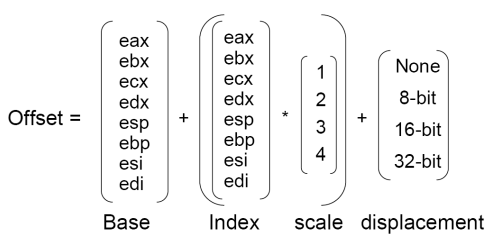
\includegraphics[scale=0.6]{immagini/address_offset}\\\\
È quindi possibile avere i seguenti casi:
\begin{itemize}
\item solo displacement: \textsf{movl foo, \%eax};
\item solo base: \textsf{movl (\%eax), \%ebx};
\item base + displacement: \textsf{movl foo(\%eax), \%ebx};
\item (index * scale) + displacement: \textsf{movl (,\%eax,4), \%ebx};
\item base + (index * scale)+displacement: \textsf{movl foo(\%ecx, \%eax, 4), \%ebx};
\end{itemize}
Ci sono anche gli operatori logici ed istruzioni aritmetiche.
\subsubsection{Meltdown in assembly}
La sintassi intel prevede di usare prima il registro dest e poi src
\begin{lstlisting}
; rcx = kernel address
; rbx = probe array

retry:
mov al, byte [rxc]
shl rax, 0xc
jz retry
mov rbx, qword [rbx+rax]
\end{lstlisting}
l'array è fatto di pagine di 4096 byte, quindi lo shift del contatore letto all'indirizzo kernel va fatto per indicizzare le diverse pagine, shiftando di 4096. Il valore trovato in rax può essere 0 se ho letto il valore 0, quindi salto su retry per rileggere lo stesso byte. Se accedo all'array, andrei nella pagina 0-esima e il valore 0 non è interessante perché è terminatore di stringa. Quindi aspetto che nella concorrenza qualcuno modifichi il valore letto. A quel punto, se non ho letto 0 carico in un altro registro quello che ho letto.\\ Speculativamente ha senso che tutto venga eseguito e che ci siano i side effects sulla cache, ma da un punto di vista reale non ha senso che venga eseguito.
\subsection{Contromisure per meltdown}
Per cercare di ovviare a queste problematiche di sicurezza dovute a meltdown:
\begin{itemize}
\item KASRL: Kernel Address Space Randomization, fa si che quando gira un applicazione, questa non sappia dove il kernel mantiene informazioni nella zona dell'address space. Se non sappiamo dove è mantenuta la chiave nell'address space del kernel bisogna andare verso attacchi bruteforce.\\ Il kernel, quando viene compilato, è pensato per avere le strutture dati e gli indirizzo a partire da una base nota. Con la randomizzazione, il kernel ad ogni statup si ricolloca a partire dalla zona nota, quindi è shiftata di un numero di posizioni che non conosciamo. Questo è possibile solo se gli accessi ai dati ed alle istruzioni in base al displacement avviene in base alla posizione relativa dall'istruction pointer.
\item KAISER, Kernel Isolation
\item Explicity cache flush ad ogni ritorno dal kernel mode: quindi se un flusso riprende il controllo dopo essere stato in kernel mode, si manda la cache in flushing. Ma possiamo avere una applicazione che, nell'asse temporale esegue come user, poi come kernel, poi di nuovo user etc... Se si fa questo la cache sta venendo buttata, quindi è come non averla in quanto viene sprecata in maniera sostanziale. Inoltre, ci sono anche attacchi che non passano per karnel.\\ La protezione può essere utile anche in un altro scenario: user eseguite in maniera malevola, quindi ci sono dei side effects che verranno osservati dopo. È possibile avere un percorso di questo tipo: eseguo, passo al kernel, il kernel esegue e mi rida il controllo. Se non valesse questa cosa, io saprei che le sys call che chiama il kernel durante quella esecuzione porta in cache dei dati che voglio attaccare. Quindi, potrei avere un attacco subito dopo la syscall.
\end{itemize}
La soluzione utilizzata ad oggi è KAISER, che sfrutta questa cosa: abbiamo analizzato le trap che possono capitare all'interno dell'attacco meltdown ovvero le memory protection violation. KAISER è tale per cui non è possibile generare quella trap per accedere a delle informazioni di zona kernel. In particolare, la page table per il programma ha le entry che afferiscono alla zona di address space user settate, mentre quelle che afferiscono alla zona kernel non sono settate e quindi generano trap di tipo page fault.\\ Ma è possibile avere una applicazione che quando esegue ha solo come pagine valide nella PT relative allo user space? No, è ideale: nell'address space, il kernel è visibile tramite la PT, il kernel non è reso tutto invisibile ma sono una zona. La zona visibile è l'unica usabile per entrare ed eseguire in modo kernel, una volta entrati si cambia la visibilità anche sul resto della zona. Quindi, in user space non si può accedere alle zone invisibili. L'implementazione attuale è la seguente: \\
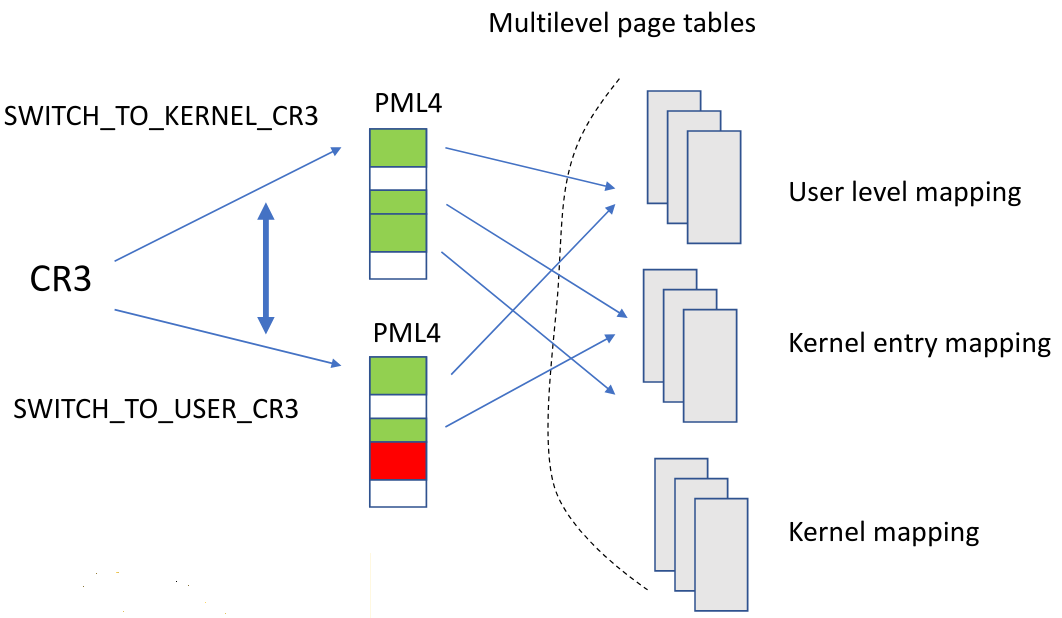
\includegraphics[scale=0.3]{immagini/KAISER}\\\\
due pt differenti, una per quando si lavora in maniera user ed una quando si lavora in kernel mode. Quando si chiama una sys call si passa ad una zona di address space in cui sono informazioni relative solo al codice kernel level, quindi non sensibile. In modo kernel, la zona di codice cambia la PT con una replicata in cui la zona è visibile, ma siamo già in modo kernel.\\ Il costo che viene pagato in termini del cambiamento della page table è che il TLB viene flushato. Nel TLB abbiamo una entry per una intera pagina, pagherò dei cache miss ma uno per pagina e non uno per ogni accesso come accade per la cache.\\ Inoltre, questa soluzione para da una serie di altri attacchi; la patch si può disattivare usando \textsf{pti=off} a livello del kernel usando GRUB. Su Linux è anche possibile mettere le patch on/off per la singola applicazione, se magari mi accorgo di un comportamento anomalo e non per tutte quelle running
\section{Branches}
Le istruzioni di salto sono un altro aspetto importante nell'esecuzione del program flow: se c'è un salto, è possibile che le istruzioni che devono entrare nel program flow provengano da diversi punti dell'address space. Quando si lavoro eseguendo in pipeline, non è possibile fillare solo quando si sa che il salto è deciso o non deciso, perché ci sarebbero stalli fino a che l'istruzione non va in commit point. I salti possibili sono riassunti di seguito 
\begin{itemize}
\item salti condizionali: non è noto se il salto avrà luogo o no quanto questa istruzione entra in pipeline. Il numero possibile di outcome però è 2: o si salta o no
\item salti non condizionali: salto sempre preso, a tempo di decode si sa già che si salta e quindi siamo in grado di acquisire le istruzioni per fillare la pipe 
\item call: anche qui il salto è sempre preso
\item return: anche questo salto è sempre preso, ma non sappiamo dove andare. Potremmo avere molte destinazioni, in quanto questo è funzione della stack area e sappiamo che il valore può essere aggiornato
\item salti indiretti: implementati in modo che l'istruzione è un salto, ma il target non è un offset nell'address space, bensì è indicato da un puntatore, quindi ad esempio il contenuto di un registro. La soluzione è molto usata quando dobbiamo realizzare dei function pointers
\end{itemize}
Quindi, eccetto i casi "più semplici" in cui si decide quando saltare a decode time, gli scenari sono più complessi perché bisognerebbe decidere dove saltare a commit time.\\ Esiste quindi nei processori il concetto di branch prediction: il processore ha osservato determinate istruzioni nella pipeline, e nel momento in cui queste vengono ri-osservate sa già cosa, in quanto ad esempio sa se nel caso precedente il salto è avvenuto o no.\\ Le architetture nei processori consentono di fare cose più complesse: quando lavoriamo in un processore pipeline super-scalare abbiamo un \textbf{dynamic predictor} che usa una Branch History Table o Branc-Prediction Buffer.\\ 
L'implementazione è basata su una cache indicizzata dai bit meno significativi dell'istruzione di salto e da un bit di stato, per cui ogni tabella ha una entry in cui viene indicato se saltare o no, e la tabella è indicizzata dal program counter. \\ Se passa una determinata istruzione viene registrato nella tabella se si è saltato o no (all'interno del bit di stato), in modo che se questa ripassa, si verifica col PC se c'è matching e se è così, in base al bit di stato, si decide quali istruzione caricare in pipeline.\\ Ovviamente, il salto può non avvenire, quindi poi bisogna flushare la pipeline se a commit time l'istruzione non salta. Siamo ancora in un contesto in cui le istruzioni lasciano tracce e sono problematici dal punto di vista della sicurezza.\\ Questa è una implementazione basica, inoltre nella tabella si mantengono solo alcuni dei bit che caratterizzano l'indirizzo contenuto nel PC: questo può far si che abbiamo un errore se prediciamo qualcosa che non si manifesterà, quindi il bit è 1 quando doveva essere 0 o viceversa, ma è anche possibile che nell'address space ci sia un'altra istruzione che ha la parte registrata nella tabella identica rispetto ad un altra istruzione che è quella effettivamente registrata e quindi abbiamo un altro tipo di errore. In generale, per errore intendiamo che vengono caricate in pipeline determinate cose e quindi si hanno dei side effects inattesi.
\subsection{Multiple bits predictors}
Il predittore ad un bit fallisce nello scenario in cui il branch viene preso frequentemente e non preso preso poco frequentemente. In questo tipo di scenario, tali predittori portano a 2 errori di seguito nella predizione, e quindi a due quashes della pipeline.\\ 
Una variante a due bit per un branch predictor ci dice che se una istruzione ha un certo indirizzo i, non registriamo un solo bit nella tabella bensì 2 bit, con cui possiamo discriminare 4 stadi possibili: 2 possono essere associati all'idea di saltare e gli altri 2 a quella di non saltare. In questo caso, per far si che venga invertita la previsione di salto, occorre avere 2 errori consecutivi\\ Possiamo quindi avere diversi outcome, ma se la macchina a stati è a 4 stati possiamo tenere traccia di più eventi possibili: ad esempio, se l'istruzione è passata ed è saltata ripassando si risalta. Se il salto non avviene, possiamo andare in un altro stato in cui viene detto che precedentemente è stato sbagliato il salto, ma si continua comunque a saltare.\\ Questo avviene ad esempio nei nested loop: c'è una volta in cui non si salta, ma le altre volte si salta sempre. Se ci fosse una macchina salta/non salta, l'ultima volta non salto e non posso ricordarmi che non ho saltato prima. Avrei quindi una serie di squash della pipeline. Un esempio di codice Assembly che realizza un loop annidato è mostrato in seguito:
\begin{lstlisting}
1	mov $0, %ecx
2 . outerLoop:
3	cmp $10, %ecx
4	je .done
5	mov $0, %ebx
6	
7 .innerLoop:
8	  ; actual code	
9	  inc %ebx
10	  cmp $10, %ebx
11	  jne .innerLoop
12
13	  inc %ecx
14	  jmp .outerLoop
15 .done:
\end{lstlisting}
Viene poi riportato l'automa a stati finiti che corrisponde al predittore a due bit:\\\\
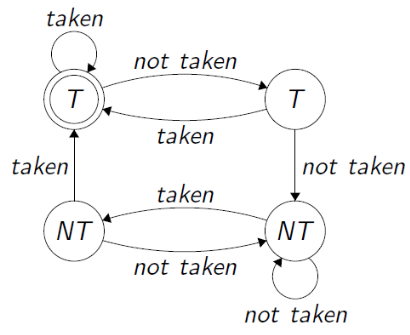
\includegraphics[scale=0.6]{immagini/2bit_pred}\\\\
Non è l'unico modo per essere efficaci nel momento in cui abbiamo dei loop nel codice: il saltare o non saltare può essere condizionato da cosa è accaduto prima. La macchina a stati sopra è riferita ad una singola istruzione, ma le cose dipendono dal passata di più istruzioni
\subsection{Altre soluzioni per branch predictors}
Se sbagliamo, su una architettura super-scalare e pipeline buttiamo decine di istruzioni magari pronte al commit, quindi è necessario andare oltre al predittore per le singole istruzioni, i due predittori che estendono il singolo sono
\begin{itemize}
\item predittori correlati a due livelli;
\item tournament predictors
\end{itemize}
Un esempio generale per considerare istruzioni di salto multiple può essere il seguente:
\begin{lstlisting}
if (aa == VAL)
	aa = 0;
if (bb == VAL)
	bb = 0;
if (aa != bb){
	// do the work
}
\end{lstlisting}
\subsubsection{Predittore correlato(m,n) a due livelli}
L'idea è che c'è una importante correlazione nel flusso di esecuzione, quindi guardando all'esempio precedente, si cerca di predire cosa accadrà nel 3° branch in base alla storia relativa a cosa è accaduto nei primi due.\\ Su architetture Intel, manteniamo per ogni flusso di esecuzione un registro di esecuzione che ci dice dati gli ultimi m salti se è avvenuto o meno il salto. \\ Il branch corrente viene predetto con un predittore ad n bit, quindi in totale ci sono $2^m$ predittori ad n bit.\\
Nella pipeline c'è quindi una maschera che registra se è avvenuto o no il salto, la maschera può essere fatta comunque da istruzioni che possono essere committed oppure speculari, quindi una zona più recente sarà committed ed una non committed. Se la storia è fatta da due bit, possiamo discriminare 4 valori differenti, collegandoli alla history sono flussi di esecuzione completamente differenti, quindi per ciascuna di queste possibilità associamo uno specifico predittore a ciascuna combinazione dei 2 bit. I predittori indicano per l'istruzione, dato cosa è accaduto nel passato per i salti, cosa fare, ovvero se saltare o meno. In generale quindi, i predittori sono tipicamente marcati con la notazione di (m,n) dove m sono gli elementi (i branch passati) mantenuti nella history ed n i bit mantenuti da ogni predittore.\\ Il predittore per la predizione corrente viene scelto sulla base dei risultati degli ultimi m branches, come è codificato nella $2^m$ bitmask.\\ Una figura riassuntiva è mostrata in seguito:\\
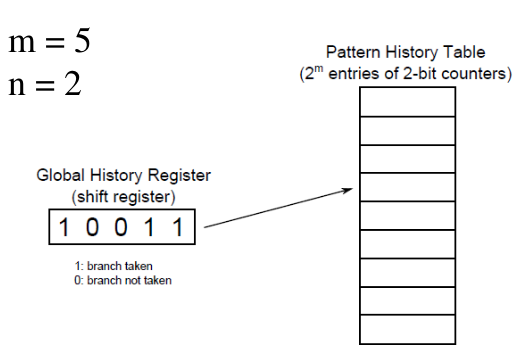
\includegraphics[scale=0.4]{immagini/corr_pred}
\subsubsection{Tournament predictor}
Il predittore di un branch tiene conto del fatto che per una istruzione di salto, a seconda di come è scritto il programma, ha senso eseguire il salto in funzione di quali sono le istruzioni passate in pipeline prima di questa. Non è detto che il predittore correlato sia sempre il migliore, perché per la singola istruzione la storia globale può essere una penalità in base alla struttura del codice.\\ Questo predittore mantiene per ogni istruzione le informazioni di un (m,n) ed anche 2 bit per avere 4 stati:
\begin{enumerate}
\item quando si predice per una istruzione di interesse, conviene guardare tutte le cose;
\item quando passa una istruzione, non guardare la history bensì solo un predittore locale;
\item guardare solo alla storia globale;
\item (non saltare)?
\end{enumerate}
Quindi, vengono messe in competizione la visione locale e quella globale. Se il flusso di esecuzione non ha molti errori, avremo una stabilizzazione che mostra "chi vince nella sfida"
\subsection{Salti indiretti}
Il salto indiretto è strano: se l'istruzione deve saltare, questo è funzione del risultato delle istruzioni precedenti, ovvero di cosa queste hanno scritto nei registri, che verranno usati per saltare.\\ Quindi, il valore di tali registri può variare sempre nel tempo, il che rende la predizione più complessa ed i side effects generati sono di più.\\ L'idea è di mantenere nella stessa architettura una cache, in cui vengono mantenute informazioni a cui associamo oltre all'indirizzo del branch anche il pre-fetched target, anche dei bit per indicare quanti errori ci sono stati.\\ Nel momenti in cui c'è cache miss non si può prelevare il salto, altrimenti viene presa l'istruzione successiva, una delle istruzioni più interessanti di questo tipo in x86 è \textsf{jump [register]}, interessante per implementare function pointers, che viene mostrata nella figura sottostante:\\
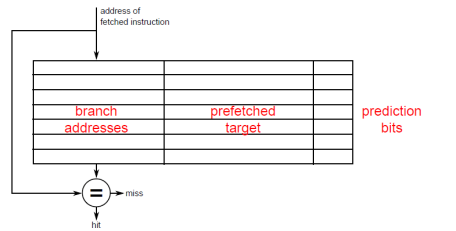
\includegraphics[scale=0.5]{immagini/jmp_reg}\\\\
Quando abbiamo un errore in predizione perdiamo performance, ed inoltre ci sono problemi di sicurezza da considerare
\subsection{Attacchi spectre}
Attacchi che ancora sono in vigore, si sta studiando come introdurre delle patch a livello hardware per poter bypassare spectre con però dei costi prestazionali importanti, ad esempio disconnettere la branch prediction dinamica. Il problema è che i dati vanno avanti, ad esempio in meltdown i dati vanno in cache e cambiano lo stato micro-architetturale.\\ In spectre accade la seguente cosa: il processore ha il branch predictor, se lo caratterizziamo come componente di più ampio livello abbiamo una fase di learning e da quello il predittore decide cosa fare la prossima volta. Ma cosa fare può essere sbagliato: insegno al predittore cosa fare in maniera volutamente errata, per poi passare un flusso dove le cose imparate non sono più valide e che quindi vengono gestite male.
\subsubsection{Spectre v1 (spectre prime}
Abbiamo un if che testa un condizione su un certo valore X, che può essere un indice usato all'interno di un array. Poi, si può scendere in un codice per cui si accede ad un array A e si usa B[X] shiftato a destra di 12, ovvero per indicizzare ogni volta 4096 byte e quindi una pagina.\\ Accediamo quindi ad A per un byte, identifichiamo il byte con B[X] ed idealmente abbiamo 256 possibilità che possono essere 256 pagine come visto in meltdown.\\ X è un indice di un'altra zona di dati, B può essere un'altra zona di memoria: sto caricando un'altra zona di informazioni spiazzandomi con X, carico il codice e usandolo per indicizzarmi in A. Quindi la posizione è in funzione di dove è B, ma anche di quanto è X: se mi sposto in una zona kernel space, funziona ancora se il branch predictor sbaglia la predizione perché è stato "allenato" così. Non abbiamo nemmeno seg fault perché è il branch predictor a fare il salto che è errato e quindi le istruzioni non vanno nemmeno in commit. Quindi, sullo stesso flusso di esecuzione possiamo fare inspection sull'array di probing A per vedere il valore che aveva B[X]. Lo spectre v1 è orientato alla problematica del branch prediction di salti condizionali.\\ Possono capitare anche cose più complesse: per come stiamo usando ora spectre, leggiamo informazioni livello kernel senza andare in seg fault, quindi il processore deve essere tale per cui l'istruzione passa comunque come offending, ma se è patchata lato hardware viene bypassata.\\ Il problema è che non basta aver risolto meltdown: quando viene eseguito del sotfware in una architettura convenzionale accade che viene chiamata una syscall ad un certo punto. Quando il  kernel parte, avrà delle informazioni nei registri di processore per sapere cosa fare, ma potrebbero essere stati scritti dei valori nel registro che viene usato in un check per cui si fanno determinate cose in base al valore, quindi il salto del kernel è impattato da tale valore e di conseguenza anche cosa la branch prediction fa.\\ Quindi, stabilito cosa deve avvenire quando si salta, si cambia il valore e questo permette di far eseguire al kernel speculativamente qualsiasi blocco di codice. Supponiamo di chiamare una syscall: a livello kernel c'è una tabella fatta di function pointers, ho passato tramite il registro quale valore della tabella considerare. Possiamo passare al branch un valore che è oltre la tabella, viene eseguito il salto perché il branch perdictor non sa che non deve andare oltre. Quindi, il codice del kernel si muove in funzione di cosa passa l'utente, ma così l'utente può passare parametri che alterano la branch prediction per poi attaccare. Quindi, la patch per meltdown è già stata bypassata, è stato necessario riscrivere il codice del kernel con patch per quanto riguarda il valore osservato livello kernel rispetto a quello passato dallo user, ad esempio marcando alcuni bit e tagliando il valore passato in modo che si rimane in zone incluse nella tabella.
\subsubsection{Spectre v2}
Con spectre si portano avanti anche attacchi di questo tipo: abbiamo il processore e gli hyperthread, ma il branch predictor sta nel "motore", non viene esposto a livello ISA. Il core è visibile da flussi differenti, nell'istante di tempo t abbiamo un programma P sul core, mentre a t' possiamo avere P' in esecuzione: la branch prediction sta nel core, quindi P può eseguire una serie di istruzioni può dare input al branch predictor per comportarsi in un certo modo, quando c'è context swtich e cambia il programma, possiamo sfruttare il branch predictor allenato, la predizione sarà sbagliata ma abbiamo side effect sul secondo contesto che è osservabile dal primo. Un riassunto dello scenario è mostrato in seguito:\\
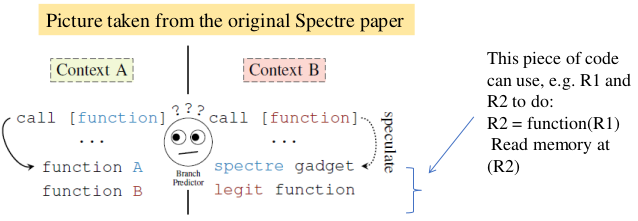
\includegraphics[scale=0.5]{immagini/spectrev2_branch_pred} \\\\
lo scenario è che l'attaccante ha costruito il flusso di esecuzione per avere l'istruzione di salto indiretto nello stesso indirizzo dell'address space rispetto a quello della vittima, quindi quando si salta, si va in istruzioni macchine dette \textbf{gadget}, ovvero delle istruzioni che possono essere utili all'attaccante in quanto vengono creati dei side effect, ad esempio se cambio qualcosa in cache e questa è accessibile all'attaccante, il cambio è visibile.\\ Il concetto di sfruttare un gadget sulla predizione è importante per la return oriented programming, dove vengono sfruttati i gadget. Ovviamente, il miss training va fatto sullo stesso CPU core della vittima, mentre il probing della cache può avvenire anche su core diversi.
\subsubsection{Come bypassare spectre v2}
Per salti diretti, l'unica cosa che il software può fare è ridurre il valore che viene passato nei registri per accedere alla memoria. Per quelli indiretti la patch è la \textbf{retpoline}, ovvero un trampolino basato su istruzione di ritorno. Supponiamo di dover lavorare con del software tale per cui quando questo esegue serve fare un salto indiretto: il salto non viene eseguito, bensì il sotfware effettivo per arrivare alla destinazione prevede l'uso di un trampolino, quindi varie istruzioni in più. I trampolini sono basati sull'istruzione di \textsf{ret}, la soluzione vale per qualunque architettura. I passi eseguiti sono i seguenti:
\begin{enumerate}
\item viene salvato nello stack il traget addrress dove saltare
\item si esegue una chiamata di un pezzo di codice che rimuove il valore di ritorno del PC dallo stack, che era la chiamata originale
\item la porzione di codice salta all'indirizzo con l'istruzione di \textsf{ret}
\item perciò, la chiamata originale non ha un ritorno attuale e quindi il codice delle istruzioni successive alla chiamata sono un loop infinito
\item i predittori per i salti indiretti per questo motivo non saranno sfruttabili per andare ad eseguire del codice in maniera speculativa
\end{enumerate}
\begin{lstlisting}
	push target_address
1:	call retpoline_target
	// put here whatever you like
	// typically a serializing instruction with no side effects
	jump lb
retpoline_target:
	lea 8(%rsp), &rsp // we do not simply add 8 to RSP
					  // since FLAGS should not be modified
	ret  // this will hit target address
\end{lstlisting}
la \textsf{lea} carica l'indirizzo effettivo, viene fatto con questa istruzione perché questa non ha side effect sul processore, eliminando gli 8 byte che rappresentano il punto di ritorno della chiamata.\\ 
\subsubsection{esempio: codice per spectre}
Nel codice, viene fatto un controllo per capire quanti cicli di CPU sono necessari per un cache hit e quanti per un cache miss. Il tempo non è comunque perfetto, perché il sistema è pur sempre time sharing e quindi fra due timer possono essere successe varie cose.\\ La secret area è una pagina che metto nell'address space per potermi poi spiazzare con x ed andare nel kernel space.
\subsection{Loop unrolling}
Il problema della branch prediction è comunque legato al fatto che vogliamo cercare di saltare prima ed inoltre ridurre il numero di branches presenti in un flusso di esecuzione: se c'è un if then else non è possibile ridurlo, ma ad esempio possiamo avere un salto condizionale dalla prima istruzione all'ultima (ciclo) e vogliamo ridurre gli impatti prestazionali da un punto di vista dei salti. Il problema è che andiamo a controllare l'esecuzione del codice e quindi paghiamo altre istruzioni macchina come overhead, per ridurre il numero di tali istruzioni viene usata tipicamente la tecnica del loop unrolling: se il ciclo deve girare per n volte, il compilatore o chi scrive il codice allarga il corpo ciclo, inserendo molteplici statements che altrimenti sarebbero eseguiti in diverse iterazioni del loop.\\
L'unrolling si può sviluppare sia a mano, ma non è buono perché stiamo scrivendo più linee di codice e quindi aumentando la probabilità di bug in quanto si lavorano in zone di memoria differenti. È anche possibile fare l'unloop in automatico, usando un tool di compilazione come gcc dicendo, prima di compilare una zona di codice, una opzione di compilazione \textsf{\#pragma GCC optimze ("unroll loops")}. Se facciamo l'unroll del loop, il ciclo viene eseguito un numero minore di volte nell'eseguibile, ma deve eseguire più attività e quindi bisogna usare più registri e magari usare più linee di cache, quindi ci può essere un più ampio impatto sull'architettura.\\ Ci sono una serie di effetti collaterali di cui tenere conto, osservabili analizzando il codice eseguibile, guardando magari nell'ELF dove è stato implementato l'unroll per verificare il fattore di unroll.
\section{Aspetti esterni al processore in una architettura IT}
Cerchiamo di capire quali sono gli impatti degli altri componenti nelle architetture IT. Siamo in uno scenario in cui abbiamo il problema del power wall: non possiamo aumentare la frequenza dei clock più di un tot perché avremo un power consumption tale per cui non avremmo più bilancio di calore nel chip.\\ Di fatti, il consumo di potenza cresce secondo la legge $VxVxF$ e per cui non si riesce ad andare sopra i 130W, limite superiore per uci is garantisce dissipazione di potenza.\\ La legge di Moore dice che si possono aggiungere transistor nella CPU per poter aumentare la potenza, ma ora non è più possibile: quindi, invece di avere un solo processore, ce ne sono di più. Nell'architettura non ci sono poi solo i processori, ma anche le memorie.
\subsection{Multi processori}
Su un multi-processore simmetrico ci sono tanti oggetti simili che possono processare un flusso di programma, vedono tutti la stessa memoria, ma hanno anche delle cache private affinché i dati siano più vicini al processore.\\ Il problema è che se il dato è lo stesso e viene avvicinato ai diversi processori, questo viene replicato e c'è un problema globale nell'interazione fra processore e memoria.\\\\
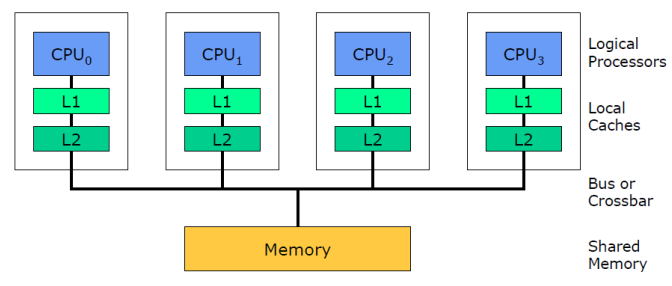
\includegraphics[scale=0.5]{immagini/multi_proc}\\\\
Ora c'è il chip multi-processor, in cui ogni processore ha più di una CPU, le CPU hanno delle L1 private e magari delle L2 condivise: questo è un modo con cui il vendor permette di accorpare le risorse del chipset rispetto al caso precedente.\\\\
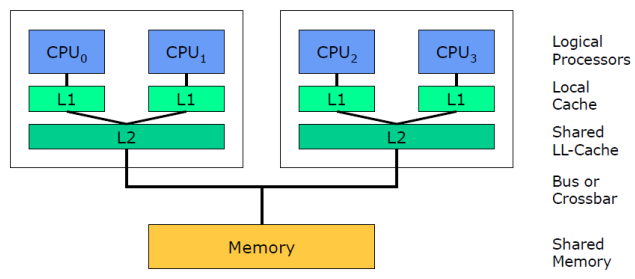
\includegraphics[scale=0.5]{immagini/cmp.png} \\\\
Infine abbiamo anche il symmetric multi-threading, perché se il core va molto veloce possiamo portare più di un flusso di esecuzione con gli hyperthread. Resta il problema dell'architettura di memoria per quanto riguarda la cache privata.\\\\ 
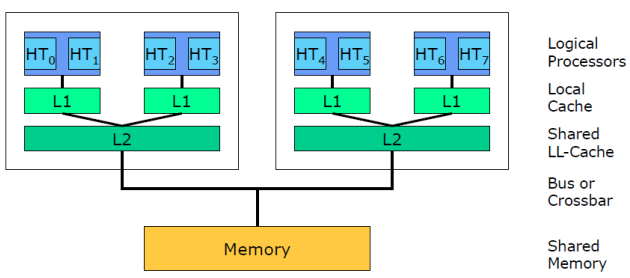
\includegraphics[scale=0.5]{immagini/smt}\\\\
Questo tipo di chipset ha fatto si che venisse scalata in verticale anche la capacità della memoria: le attività che portano sulla memoria fanno traffico su un unica strada e questo ha portato alla creazione dell'architettura NUMA
\subsection{Architettura NUMA (Non Uniform Memory Access)}
La memoria è composta da vari slot e ciascuno ha una via principale per portare dati verso il processore. Inoltre, ogni processore può leggere dati dagli slot non vicini a lui, ma deve farlo tramite una via esterna alla sua. Supponiamo che il core 1 debba usare solo pagine della zona di memoria a lui vicine, allora le due zone di memoria toccate sono separate e riusciamo a raddoppiare la capacità computazionale della memoria.\\ Il problema è quando vanno toccate zone di memoria non direttamente: servono strutture di interconnessione ed inoltre bisogna bloccare la strada per quel nodo NUMA da parte del core ricevente.\\ Lavorando in una architettura NUMA, i dati numerici ci dicono orientativamente che si aspetta dai 50 ai 200 cicli di clock per ricevere dei dati dalla memoria se si accede ad una zona vicina, altrimenti si va sui 200\%300 cicli. Si parla di sistemi scarichi, quindi aumentano parecchio se le vie sono busy per via del carico sul sistema.\\
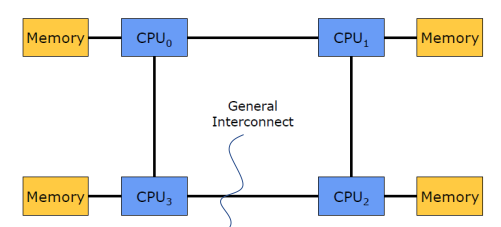
\includegraphics[scale=0.5]{immagini/numa}
\section{Coerenza delle cache}
Le attività basiche che caratterizzano l'hardware riguardano quello che avviene nella zona di cache: questa non è visibile nell'ISA, non è possibile toccare direttamente la cache col software per cui non si ha in maniera esplicita la possibilità di governarla.\\ C'è il problema della coerenza delle cache: la cache è un sistema di replicazione, quindi astraendo la struttura interna abbiamo un insieme di slot messi a disposizione per mantenere dati. Il dato D può essere registrato in due slot diversi, quindi quale replica si usa se qualcuno chiede di leggere un dato? Ancora peggio se avviene una scrittura sul dato: si aggiorna una sola replica o entrambe? Altra cosa interessante è che quando si parla di coerenza della cache si parla solo dell'oggetto hardware cache, ma nella CPU avvengono diverse cose (ooo, speculation etc...), ad esempio le scritture vengono fatte sullo store buffer e vengono poi portate in memoria e questo problema riguarda la \textbf{memory consistency}.
\subsection{Definizione della coerenza}
La coerenza nell'architettura di cache è definita in base a 3 proprietà:
\begin{itemize}
\item stiamo leggendo da una locazione di memoria X, precedentemente scritta dallo stesso processore ritorna l'ultimo valore scritto se nessun altro processore ha fatto nulla su quella locazione. \textbf{Causalità del program flow.}
\item {Avoidance of staleness}: se leggo da X e la lettura segue una scrittura su X da un altro processore, il valore letto è quello che è stato scritto dal processore se le due operazioni sono separate da un certo intervallo temporale
\item Tutte le scritture su X da tutti i processori sono serializzate, quindi non si possono vedere le write dai diversi processori in ordine diverso. Quindi viene gestito un ordine in modo che i dati vengano acceduti col valore corretto dai diversi processori quando c'è un update; non ci sono buffer dove vengono mantenute le cose e non vengono rese effettive (come accade ad esempio nello store buffer)
\end{itemize}
\subsubsection{Cache write through e write back con le consistenze}
Cosa accade, rispetto alla memoria, quando viene scritto un dato. Vediamo se le cose fatte da un single core basta anche per un multi-core. I due processori hanno due cache e c'è poi la memoria, vediamo la tecnica del \textbf{write through}, per cui il valore scritto in locale viene anche propagato sulla memoria.\\
Se ci muoviamo con più componenti associate a processori differenti, possiamo avere che: $CPU_0$ legge X e carica 0 in cache, fa lo stesso $CPU_1$. Poi, $CPU_0$ scrive 1 su X e propaga la scrittura, ma quando $CPU_1$ legge X dalla cache legge 0 e la distanza fra le due operazioni può essere arbitraria, stiamo violando il requisito 1.\\ 
Se usassimo write back: $CPU_0$ legge X e carica 0, $CPU_1$ legge X e carica 0. Poi $CPU_1$ scrive 1 e la scrittura non viene propagata, poi $CPU_1$ scrive 2 su X. Quindi abbiamo due valori aggiornati, uno in memoria, se $CPU_1$ fa il write back della linea in cui c'è X e poi successivamente lo fa anche $CPU_0$, il valore 2 viene sovrascritto e quindi siamo in grado di invertire l'effetto dell'update sui dati indipendentemente dalla distanza temporale fra gli update.
\subsection{Protocolli di consistenza}
Le cache, oltre a mantenere i dati eseguono anche dei protocolli, quindi la logica di controllo nella cache è più articolata della letture/scrittura cache. Sono implementati a livello firmware, ed hanno 
\begin{itemize}
\item una serie di transazioni che sono supportabili fra diversi componenti hardware
\item gli stati in cui si può trovare un blocco di cache
\item un insieme di eventi gestiti dal controller
\item un insieme di transizioni fra stati
\end{itemize}
L'architettura può essere organizzata in maniera differente in base a diversi fattori
\begin{itemize}
\item topologia dell'interconnessione
\item primitive di comunicazione
\item gerarchia di memoria, se inclusiva o no
\item politiche di cache
\end{itemize}
i protocolli possono poi migliorare diverse performance
\begin{itemize}
\item latenza della singola transazione
\item throughput 
\item overhead dello spazio dovuto ai bit di gestione, che toglie spazio alla cache effettiva
\end{itemize}
Le famiglie classiche di protocolli sono due, che risolvono il problema di quando aggiornare le repliche nelle altre cache 
\begin{itemize}
\item invalidate protocols: quando un core scrive un blocco, tutte le altre copie diventano invalide, questo implica che si evitano le situazioni descritte prima. Solo il writer ha la possibilità di accedere alla copia aggiornata. Si incrementa la latenza ma si riduce la banda utilizzata, però chi vuole il dato non lo ha vicino nei componenti dell'architettura di caching
\item update protocols: quando avviene una scrittura, vengono aggiornate tutte le altre copie. Si pagano però costi importanti per l'aggiornamento dei dati: ogni copia del blocco è sempre aggiornata alla copia coerente. Abbiamo il trade-off fra banda e latenza: ognuno prende la copia dal vicino ma si paga sulla banda
\end{itemize}
I primi sono quelli usati in architetture moderne, per cui ci focalizziamo su quelli per capire come avviene l'invalidazione
\subsubsection{Snooping cache}
Come lavorano effettivamente i vari componenti dell'architettura hardware per implementare l'invalidate protocol: tutti i componenti sono connessi fra loro tramite un mezzo broadcast, anche detto rete, quindi tutte le cache possono parlare con tutte. È un modo semplice per poter prendere il mezzo, comunicare a tutti ad esempio un cambio di stato per far si che tutti lo cambino. C'è la serializzazione di tutte le transazioni: quando la CPU va sull'interfaccia verso la cache, l'interazione deve usare il broadcast medium, ma se non è necessario che ci sia la transazione distribuita non si parla. Se quando si manda l'interazione verso l'architettura di cache e questo genera un evento tale per cui qualcun altro deve parlare c'è la serializzazione, quindi nella time line i cambi di stato avvengono quando quello precedente è completato. I componenti di caching sono connessi a dei controller che è in grado di capire i messaggi di broadcast per poter effettuare i cambi di stato. Finché il controller non ha preso il mezzo di comunicazione il cambiamento di stato non può avvenire. Di seguito, viene mostrato uno schema architetturale:\\\\
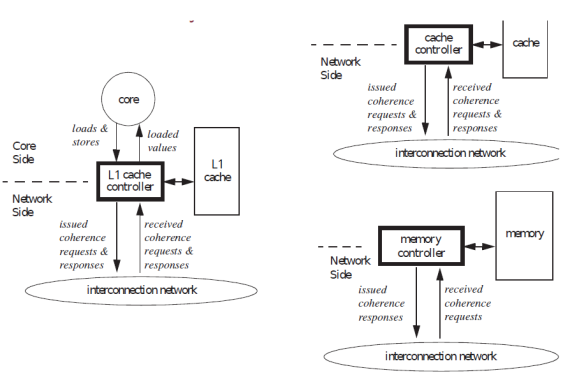
\includegraphics[scale=0.5]{immagini/cache_conn}\\\\
Le azioni trattano le singole linee di cache, per cui quando qualcuno parla lo fa per quella linea di cache.
\subsubsection{MSI protocol}
Tipicamente, si tiene traccia dei seguenti stati per un blocco in cache:
\begin{itemize}
\item modified, ovvero scritto e quindi che rende invalide le altre copie
\item invalid
\item shared: la versione più è condivisa fra vari componenti, qualcuno ha avuto una copia dal writer o da un altro reader
\end{itemize}
Una transazione di scrittura invalida tutte le altre copie del blocco di cache, mentre una transazione di lettura
\begin{itemize}
\item prende l'ultima copia aggiornata dalla memoria in caso di cache write thorugh
\item prende l'ultima copia aggiornata dalla memoria o da un altro componente  di caching nel caso write back (come ad esempio in Intel)
\end{itemize}
\subsubsection{Protocollo MESI}
Gli stati di una linea di cache possono essere 4
\begin{itemize}
\item Invalid
\item Modified
\item Shared
\item Exclusive: il componente di cache indica che fa una gestione esclusiva di quella linea di cache. Ovvero quel componente può fare ciò che vuole senza dover dire a nessuno che ha scritto la linea. Quindi, questo può avvenire senza interazioni con nessuno: se un program flow tocca un dato per aggiornarlo di continuo, non è necessario comunicare ad altri componenti che questo è accaduto, e prende di conseguenza la linea di cache ad uso esclusivo
\end{itemize}
Quindi, non è vero che qualcuno legga qualcosa di vecchio, perché questo è vero solo se qualcuno passa ad exclusive e rende invalide le altre copie.\\ L'automa a stati finiti che riassume il passaggio fra i vari stati è mostrato di seguito:\\\\
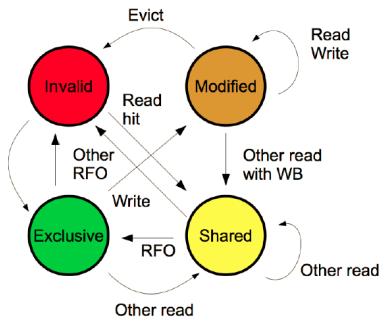
\includegraphics[scale=0.5]{immagini/MESI}\\
una RFO non è altro che una richiesta di ottenere l'ownership della linea di cache.\\
\textbf{esempio: transazioni in risposta a letture locali}\\
se lo stato è M, E o S non succede nulla. Se invece siamo in I, va generata una richiesta sul bus, se ci sono altre cache che hanno una copia del dato mandano un segnale di sharing e se questo avviene, il componente transita nello stato S; altrimenti, va nello stato E.
\textbf{esempio: transazioni in risposta a scritture locali}\\
\begin{itemize}
\item se lo stato è M non ci sono transazioni
\item se lo stato è E non ci sono transazioni sul bus e si fa in M
\item se lo stato è S, la linea è in locale ma posso avere le altre copie e quindi tramite l'uso del bus genero una richiesta di read per prendere l'uso esclusivo
\item se lo stato è I si genera una richiesta di uso esclusivo e si va in M
\end{itemize}
ALTRI ESEMPI SULLE SLIDES
\subsubsection{MOESI}
Variante del MESI in cui c'è uno stato in più che è Owned, ovvero una cache line può essere Owned e la differenza rispetto ad Exclusive è che se aggiorno della linea di cache, gli altri la hanno invalida. In O è possibile che se aggiorno la linea do la copia a chi la chiede ma lo avviso che essendo l'owner potrei aggiornare la linea in futuro e che chi al riceve non può più aggiornarla; questo evita la transizione in diversi stati come avveniva prima.
\subsubsection{Implementazioni in x86}
Tipicamente, in Intel
\begin{itemize}
\item MESI
\item Cache inclusive
\item Write back
\item Cache L1 con linee a 64 byte
\end{itemize}
AMD
\begin{itemize}
\item MOESI
\item Cache esclusiva ad L3
\item Write back
\item Cache L1 con linee a 64 byte
\end{itemize}
\subsubsection{Alternativa allo snooping}
Lo snooping va bene quando la scala dell'architettura non è grande, ma se la scala cresce e si parla tutti con tutti ci sono problemi di delay.\\ Quindi, lo snooping non scala bene, per cui si risolve usando soluzioni \textbf{directory-based}:
\begin{itemize}
\item non c'è più il broadcast, i componenti comunicano indirettamente fra loro
\item al centro della comunicazione c'è la directory, che mantiene i meta-dati
\end{itemize}
Quindi, per parlare con i componenti, non è detto che debba parlare con tutti ma lo faccio solo con la directory. Inoltre, la directory serializza tutte le attività solo internamente.
\paragraph{Funzionamento della directory:}per ogni unità portata dalla RAM alla cache, vengono mantenuti dei meta-dati, dove indichiamo che sta mantenendo la copia del dato e se il dato è dirty.\\\\
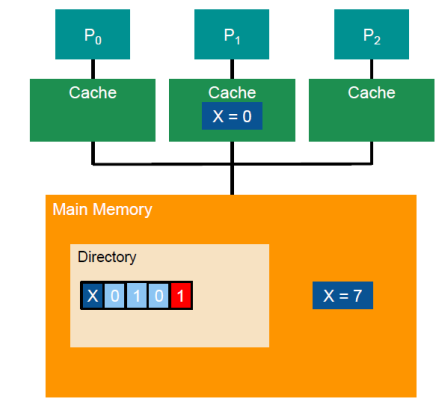
\includegraphics[scale=0.5]{immagini/dir_based}\\\\
Possiamo quindi dire che c'è una versione aggiornata presso un componente della cache, che è in corrispondenza di chi ha il dato aggiornato (l'1 azzurrino) e quindi poi si aggiorna, se qualcuno richiede il dato, chi lo mantiene.\\ \textbf{esempio:}\\ Abbiamo un read miss per $P_0$, quindi andando dalla directory scopre chi ha la copia del dato, consegnarlo e marcare il bit pari ad 1. In questo modo, sappiamo che quando qualcuno scrive dobbiamo invalidare solo alcuni dei processori ovvero quelli che hanno il dato shared.
\subsection{Relazione fra software e performance della cache}
La scrittura del software produce un program flow che poi finisce in cache, a seconda di ciò che viene scritto. Supponiamo di avere un program flow in cui si cerca di accedere in memoria per prelevare un dato e quel dato è in una certa linea di cache. Supponiamo poi di avere un altra istruzione che vuole leggere un altra area di memoria, quindi in corrispondenza di un'altra linea di cache: abbiamo la località dei dati user space\\ Il problema è grave se giriamo con più thread o hyperthread o più processi in concorrenza che accedono in memoria: le istruzioni chiamate toccano le stesse strutture dati, le interazioni chiamate cambiano lo stato MESI delle linee di cache, quello che bisogna evitare quando si scrive codice di kernel è che i dati usati più spesso devono essere sulla stessa linea di cache in modo da diminuire gli accessi in cache.\\ Le informazioni scarsamente correlate fra loro non devono invece cadere sulla stessa linea di cache, perché se due thread vogliono scrivere su due diversi byte e questi sono nella stessa linea di cache interagiscono con il protocollo MESI chiamando un maggiore numero di transazioni, sharando la linea di cache.\\ In modo che il software sia scritto bene, occorre sapere se l'area di memoria logica è allineata con la linea di cache: viene dato un pointer dalla malloc e vogliamo che i 64 byte logici che otteniamo siano allineato coi 64 byte della linea di cache così da avere un buffer cache aligned. Questo dipende dal tipo di allocatore che si usa:
\begin{itemize}
\item \textsf{posix\_memalign }
\item \textsf{aligned\_alloc }
\item \textsf{valloc }
\end{itemize}
C'è quindi il problema del false cache sharing: se abbiamo due strutture che sono una di x byte ed una di y byte e questi sono usati da due core diversi, e la somma x+y $<$ 2*chache\_line, i dati cadono sulla stessa linea di cache e quindi c'è un problema prestazionale.\\ 
\subsection{Insepction cache line access}
Abbiamo visto meltdown e spectre, tutto è nato usando il risultato dell'inspecting cache line access, ovvero è possibile con questa tecnica che si basa sull'osservare le latenze di accesso alle aree di memoria condivisa capire se un dato è in cache oppure no. Per fare questo, si possono utilizzare i passi seguenti:
\begin{itemize}
\item il contenuto della cache relazionato ad un certo dato condiviso fa flushato
\item si ri-associa il contenuto in read mode
\item osserviamo la latenza di accesso: se è bassa, vuol dire che qualcun altro ha portato il dato in cache, altrimenti  ce lo sto portando io
\end{itemize}
L'implementazione su x86 è basata su due blocchi fondamentali:
\begin{itemize}
\item un timer ad alta risoluzione, per effettuare le misure temporali
\item usare istruzioni non privilegiate per fare cache line flush
\end{itemize}
\subsubsection{High resolution timer per x86}
Esiste un high resolution timer, che permette di misurare con una grana fine, ovvero quella dei cicli di clock, quando tempo è passato.\\ Il cronometro è RDTSC, si accede ad un registro special purprose che mantiene il numero di cicli di clock passati fino a quel momento (può andare in overload), il valore è mantenuto in un registro della famiglia msr, ovvero dei registri non-general purpose. I valori vengono caricati in edx ed eax, 32 bit in uno e 32 bit nell'altro, che siano i più o meno significativi della maschera di 64 bit del contatore, quindi possiamo prendere una delle due parti in base al nostro interesse.\\ Nella pagina del manuale di x86 viene detto che l'istruzione può non essere permessa quando si lavora user mode, generando un protection error, scrivendo un bit in CR4 per cui resettando o settando il bit è possibile che l'istruzione sia o non sia usata user mode. L'istruzione è molto usata da software che fa profiling dell'applicazione, quindi è necessario lasciare la possibilità che sia usata user mode, per cui ci si espone al fatto che possa essere usata da software malevoli.
\subsubsection{Cache line flush}
L'istruzione per fare cache line flush è CLFLUSH: viene passato un pointer ad un byte, che è in una zona di 64 byte che in memoria fisica costituiscono una unica linea che viene caricata, quindi la linea viene flushata. Se viene chiamata l'istruzione, siamo sicuri che l'operazione sia corretta rispetto a tutte le operazioni che sono state fatte su quel byte e su quella linea? Siamo in una finestra temporale in cui, prima del flush, avevamo cominciato una write che poteva aver toccato un byte di quella stessa linea, ed in pipeline le due istruzioni potrebbero essere invertite, per cui se non stiamo attenti rischiamo di flushare un contenuto vecchio, che poi verrà riscritto. Quindi, per poter riportare in memoria con la flush l'istruzione scritta e quindi quella aggiornata, bisogna usare una ulteriore istruzione: MFENCE. Con questa istruzione, stiamo cambiando il modo con cui il processore sta accedendo alla cache.
\subsection{ASM inline}
Come si scrive Assembly in modalità C: è possibile mischiare notazione C e Assembly, quando verrà eseguita la versione della funzione alcune istruzioni Assembly saranno già state scelte dal programmatore.\\ Tipicamente un blocco ASM prevede alcune informazioni obbligatorie ed altre opzionali. Vediamo il blocco:
\begin{lstlisting}
__asm__ [volatile] [goto] (AssemberTemplate
		[ : OutputOperands ]
		[ : InputOperands ]
		[ : Clobbers ]
		[ : GotoLabels ]);
\end{lstlisting}
Output ed Input permettono di rapportare l'esecuzione delle istruzioni specificate nell'Assembler template, ovvero qualcosa che avvenga prima o dopo. I clobbers è l'insieme dei registri che eventualmente devono essere salvati se c'è un side effect, quindi che siano push e pop per rimettere a posto lo stato. Volatile va a dire al compilatore di non andare ad ottimizzare le istruzioni macchina passate, cosa che altrimenti può avvenire in automatico.\\ Dettagli su Input/Output
\begin{itemize}
\item il simbolo uguale può essere usato in fase di output, quindi ad esempio che si sta relazionando una variabile ad un registro in output
\item nella zona di input non è necessario usare il simbolo di =, andando a specificare movimenti di variabili differenti
\item per specificare se usare registri o memoria al compilatore, ci sono delle notazioni apposite:
\begin{itemize}
\item r: registro generico
\item m: area di memoria generica
\item 0-9: indici per riferire cose usate prima nella notazione
\item i/l sono gli immediate a 32 o 64 bit
\item q: registri byte addressable
\item A: eax o edx
\item altro...
\end{itemize}
\end{itemize}
Dato tutto questo, ecco come viene riscritta la flush + reload:
\begin{lstlisting}
usigned long probe(char *adrs){
	volatile unsigned long cycles;
	asm(
		"mfence \n"
		"lfence \n"
		"rdtsc \n"
		"lfence \n"
		"movl %%eax %%esi	\n"
		"movl (%1) %%eax	\n"
		"lfence \n"
		"rdtsc \n"
		"subl %%esi, %%eax \n"
		"clflush 0(%1)		\n"
		: "=a" (cycles)
		: "c" (adrs)
		: "%esi" , "%edx"   );
	
	return cycles;
}
\end{lstlisting}
la mov dell'1 dice che va preso il valore di ecx ed usarlo come pointer per caricare il valore in eax, quindi è la load di cui vogliamo misurare il tempo. Va preso il cronometro prima e dopo con rdtsc. Sposto anche dei dati per fare la sub, ovvero sottraendo i cicli di clock iniziali e finali.\\ Di seguito, vengono mostrate delle tipiche timelines che si possono avere durante l'esecuzione di un flush+reaload.\\\\
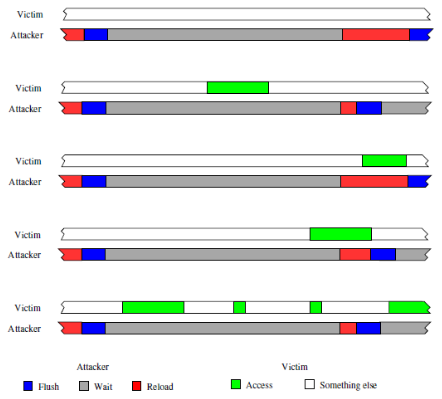
\includegraphics[scale=0.5]{immagini/flrel}
\subsection{Inspection cache senza RDTSC}
Quando usiamo RDTSC, misuriamo dei valori assoluti: vedendo insieme i due valori ottenuti per accesso ai dati con e senza flushing, e vediamo che uno scenario è circa 3 volte più lento di un altro. Potremmo quindi anche non misurarli correttamente ed avere una misura indicativa di cosa accade. Quindi, se viene prevenuto l'uso di RDTSC, i tempi possono essere misurati secondo un altro schema:
\begin{itemize}
\item usiamo più thread: uno dei due incrementa solo una variabile, l'altro invece fa flush e reload ed il tempo viene misurato usando il valore passato dal primo thread, per vedere se viene incrementato di più o di meno. Come facciamo per far si che il thread non riesca a determinare la differenza fra i due casi: se il thread non è in CPU quando il secondo thread cerca di prendere il valore della misura, allora la differenza sarà sempre 0.
\end{itemize}
\subsection{Nota: inclusività della cache}
La cache inclusiva è tale per cui ad un livello più baso il componente di caching $L_x$ ha sempre una copia aggiornata del contenuto cachato dal livello superiore $L_y$, quindi $L_y$ è sempre incluso in $L_x$.\\ Per sistemi che usano cache non inclusive potrebbero causare il fallimento di attacchi di tipo flush + reload, che possono continuare ad essere fruttuosi se, ad esempio, lanciati su processi che girano sullo stesso CPU core.
\section{Memory concistency}
Abbiamo visto la cache coherency, che ci ha fatto vedere cosa accade in una architettura in quanto abbiamo processore $|$ zona memorizzazione con i vari componenti (L1, L2, RAM) quando qualcuno chiede o aggiorna dati.\\ Osservare cosa succede guardando solo l'interfaccia fra processore e memoria da una visione limitata di cosa accade realmente quando un program flow deve lavorare con la memoria. \\ Quindi può accadere che su un program flow operazioni di accesso in lettura e scrittura non siano riversate sull'interfaccia quando pronte. Noi ci aspettiamo che una lettura riporti l'ultimo valore scritto, ma sull'interfaccia o da parte del program flow? Perché se ci sono più flussi paralleli questo cambia: se ad esempio una istruzione che scrive con una mov, non è detto che il risultato sia subito esposto sull'ISA, ma può essere scritto nello store buffer. Quindi se un processore P scrive e P' legge, può darsi che la lettura di P' venga postata sull'interfaccia per leggere, ma il valore di P non è stato ancora scritto.\\ Abbiamo due aspetti:
\begin{itemize}
\item program ored, ovvero l'ordine di accessi in memoria per come accadono nel program flow
\item visibility order, ovvero l'ordine con cui i processori accedono per andare sull'architettura moderna e che viene osservato da uno o diversi processori. Ogni lettura restituisce il valore della scrittura più recente
\end{itemize}
\subsection{Sequencial consistency}
Una modalità di raccordare le cose è la sequencial consistency, in cui essenzialmente per tutto ciò che viene fatto su un program flow non è possibile che una cosa fatta non sia visibile dagli altri flussi su un oggetto condiviso, ovvero sulla memoria.\\ Supponiamo di avere un flusso di programma che scrive su A ed uno che scrive su B, ed un altro scrive su C, non è vero che se guardo il visibility order per gli altri c'è prima B e poi A o C: l'ordine è A-C-B.\\ Un altro esempio:
\begin{itemize}
\item la $CPU_1$ esegue le operazioni
\begin{itemize}
\item [A] = l;($a_1$)
\item [B] = l;($b_1$)
\end{itemize}
\item mente la $CPU_2$ fa
\begin{itemize}
\item u = [B];($a_2$)
\item v = [A];($b_2$)
\end{itemize}
\end{itemize} 
Se l'ordine con cui vengono viste le operazioni, e quindi i risultati, è $a_1, b_1, a_2, b_2$ allora c'è sequencial consistency. Se invece l'ordine è, ad esempio, $b_1, a_2, b_2, a_1$ non c'è sequencial consistency.\\
Le architetture che abbiamo non sono sequencially consistents: se scriviamo un valore e mandiamo in commit l'istruzione e poi scriviamo in una seconda istruzione, potremmo usare una linea di cache differente per la seconda istruzione e non necessariamente aspettare in MOESI/MESI, quindi se dobbiamo servire dei cache miss e non c'è la possibilità di lavorare sulla linea di cache come si vorrebbe, bisogna fermare altre attività.
\subsection{Total Store Order}
Nelle architetture moderne, si lavora col Total Store Order: quando mandiamo delle scritture, queste possono scrivere in uno \textbf{StoreBuffer} intermedio e solo poi tali scritture sono riportate in memoria. Come vengono riportate è deciso dal vendor, può essere l'ordine con cui sono arrivate le cose oppure no.\\ Quindi, se lo StoreBuffer è Out-Of-Order è ancora più complicato la relazione fra program order e visibility order. Le macchine moderne tipicamente hanno questo StoreBuffer, quindi a valle della registrazione nel buffer alcune scritture vengono ritardate. Lo store buffer va bene se scrivo e leggo la stessa cosa, ma è diverso se occorre leggere da altre aree di memoria. \\ Processori x86 tipicamente implementano lo \textbf{store bypass}: una istruzione scrive nello StoreBuffer, un'altra che legge lo fa direttamente dalla memoria, ma così nel visibility order non è rispettata la consistenza sequenziale.\\ Lo StoreBuffer è utile per evitare di dover per forza ogni volta di interagire con una memoria per le scritture, se ad esempio il valore serve al program flow viene ripreso direttamente dallo StoreBuffer. Aiuta quindi nelle performance, ma c'è il problema della consistenza da gestire.\\ Un esempio di algoritmo che non funziona senza sequencial consistency (Algoritmo di Dekker):\\\\
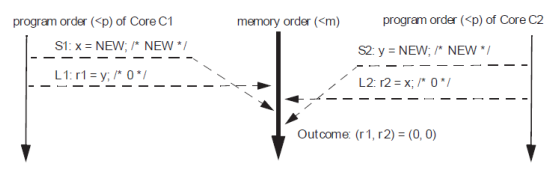
\includegraphics[scale=0.5]{immagini/dekker}
\\ Ognuno segnala una variabile e legge quella dell'altro
\subsection{Sincronizzazione della memoria in x86}
Il problema va affrontato processore per processore, perché caratterizza l'architettura del processore stesso. Occorre gestire lo StoreBuffer, in x86 lo si può fare con delle apposite istruzioni macchina
\begin{itemize}
\item SFENCE: store fence, permette di fare qualcosa per quanto riguarda la visibilità delle cose che sono nello StoreBuffer. Quindi, si dice che tutte le store precedenti alla sfence devono essere rese visibili prima che vengano mostrare quelle dopo l'sfence. Questo permette quindi di gestire idealmente degli StoreBuffer non FIFO, rendendoli quindi FIFO ma in molte implementazioni Intel lo usano già;
\item LFENCE: mentre sfence lavora sulle store, lstore lavora sulle load. La specifica di manuale non parla del visibility order, lfence permette invece di riorganizzare l'ordine di esecuzione delle load: lfence non esegue finché le load precedenti ad lfence non sono complete, ma anche nell'ordine speculativo. Quindi possiamo sincronizzare le istruzioni di load nella pipeline. Qui non si parla di visibilità globale, è importante per quando misuriamo delle latenze
\item MFENCE: Nessuna fra lfence ed sfence permettono di risolvere lo \textbf{store bypass}, ovvero la possibilità che delle operazioni di load superino delle scritture e quindi vengano lette delle informazioni stale. \\ Con mfence si sincronizzano tutte le attività verso la memoria, ovvero dallo store buffer verso la memoria, ma anche le letture verso al memoria. Evitiamo quindi il problema dello store bypass
\end{itemize}
Questo è fondamentale quando si scrive codice del kernel, perché siamo concorrenti su tutti i core. \\ Ci sono una serie di istruzioni che permettono di sincronizzare load e store: se ad esempio consideriamo una MFENCE, questa permette di scaricare un load buffer in memoria, ma ci sono delle istruzioni che fanno cose più complesse: lettura di una zona di memoria ed aggiornamento del valore. Quindi ad esempio possiamo leggere valori, confrontarli con delle bitmask e se il confronto va a buon fine, aggiornare il valore. Le istruzioni sopra permettono di fare questo, inoltre possiamo prendere lo StoreBuffer e scaricarlo in memoria in modo che tutti i dati precedenti siano andati in memoria. \\ Abbiamo, fra le tante, \textbf{CMPXCHNG}: l'operazione prende un valore, lo porta nel processore, lo compara e poi lo aggiorna. Ci si aspetta che tutto ciò si basi sul fatto che il valore che viene preso per compararlo sia il dato aggiornato, quindi la linea di cache va bloccata a tutti gli altri processori, per essere letta ed aggiornata atomicamente. Questo è implementato in x86, ma va anche a flushare ciò che è nello store buffer ed è generato da istruzioni precedenti, per cui si sincronizza la memoria. \textbf{CMPXCHNG} permette di implementare i lock, in modo che se viene trovato lo 0 nella locazione, ci mette un 1 e prende il lock; controllando il bit di stato della CPU è possibile capire se la compare\&swap è andata a buon fine, in modo da sapere se è stata presa la linea di cache.\\ Possiamo ridurre il costo di questa istruzione macchina, in modo che non mantenga la linea bloccata in stato exclusive, tramite il prefisso \textsf{\textit{lock}}.\\  Più in generale, le istruzioni che fanno questa attività si chiamano istruzioni della classe \textbf{Read-Modify-Write}: tre operazioni insieme, ce ne sono varie che possono fare diverse cose. La osa interessante è che quando viene eseguita una operazione di questo tipo, si interagisce con MESI, perché bisogna andare sull'interfaccia CPU-memoria e prendere la linea di cache in maniera esclusiva, verranno quindi spesi diversi cicli di clock per fare questa attività e quindi bisogna stare attenti all'uso delle operazioni perché impattano sulle performance. I costi spesi ci sono: bisogna flushare lo StoreBuffer in memoria, quindi la linea di cache da scrivere deve transitare nello stato giusto, quindi di deve interagire col MESI. La cosa interessante è che però si lavora solo in cache, quindi non si blocca l'accesso in memoria.
\paragraph{gcc built-in}ci sono una serie di intrincisc gcc che permette di usare una API da usare nel codice in modo che il programmatore sia più vicino a ciò che accade nell'architettura hardware, viene indotto qualcosa.
\subsubsection{Esempi di implementazione}
Vediamo l'implementazione di una \textbf{Active Barrier}, che è una barriera fra thread per ottenere sincronizzazione. 
\begin{lstlisting}
long control_counter = THREADS;
long era_counter = THREADS;

void barrier(void){
	int ret;
	
	while(era_counter != THREADS && control_counter == THREADS);
	ret = __sync_bool_compare_and_swap(&control_counter,THREADS,0);
	if(ret) era_counter = 0;
	
	__sync_fetch_and_add(&control_counter,1)
	while(control_counter != THREADS);
	__sync_fetch_and_add(&era_counter,1)
}
\end{lstlisting}
Se occorre controllare un certo numero di threads, si scrivono due variabili control\_counter ed era\_counter, perché è possibile che il thread esca dallo schema prima degli altri, quindi se rientra si porta all'era successiva ma qualcuno può ancora usare l'era precedente. Il thread che vuole scrivere sulla memoria cerca di portare control\_counter a 0, dopo esserci riuscito ( e solo uno ci riuscirà alla volta) cambia anche l'era\_counter per impedire anche allo stesso thread di rientrare finché anche gli altri non sono rientrati. In control\_counter viene aggiunta una unità, in modo che tutti gli altri thread aspettino che tutti passino.\\\\ 
Un altro esempio è la \textbf{trylock basata su ASM}:\\
\begin{lstlisting}
int try_lock(void * uadr){
	unsigned long r = 0;
	asm volatile(
		"xor %%rax,%%rax\n"
		"mov $1,%%rbx\n"
		\textbf{"lock cmpxchg %%rbx,(%1)\n"}
		"sete (%0) \n"
		: : "r"(&r), "r" (uadr)
		: "%rax","%rbx"	
	);
	return (r) ? 1 : 0;
}
\end{lstlisting}
la C\&S è basata sul valore di rax, usiamo poi l'indirizzo per accedere alla memoria (\%1 = uadr) e rax è il registro di comparazione. Alla fine, viene ritornato 0 o 1 a seconda del valore ottenuto da r, quindi è possibile poi riprovare la trylock se non viene preso il lock.
\subsection{Locks contro coordinazione scalabile} 
In una architettura moderna è necessario considerare che una memoria può essere acceduta da più thread. Fin ora abbiamo risolto con dei lock, ma l'approccio non è vincente se il numero di thread concorrenti diventa molto alto ed inoltre i thread potrebbero essere interessati a zone differenti della struttura dati, se usiamo i lock uno dei thread viene bloccato e questo è un problema di scalabilità importante. Sono nati da molto tempo degli approcci in cui il coordinamento si sfruttano istruzioni RMW non per implementare il lock bensì gli step da eseguire nella struttura dati, quindi l'algoritmo di gestione della struttura dati. Lavoriamo su due zone separate, la cosa è coerente perché i thread sanno di essere gli unici a lavorare sulla memoria, le soluzione che abbiamo sono
\begin{itemize}
\item Read Copy Update (RCU) usate in maniera massiva nel kernel Linux
\item Coordinamento non bloccante, dove abbiamo algoritmi di tipo lock e wait free. Non vengono usati i lock, quindi si lavora su una struttura dati condivisa secondo delle regole differenti
\end{itemize}
I meccanismi garantiscono che quando vengono rilasciati i lock, le modifiche contenute nello StoreBuffer sono state flushate in memoria.
\subsubsection{Linearizzabilità}
Criterio di correttezza di un algoritmo, se l'algoritmo è linearizzabile è corretto. Stiamo ragionando sulla concorrenza di threading, possiamo avere che tutto ciò che facciamo in un algoritmo linearizzabile è simile a ciò che faremmo in un algoritmo serializzabile. Il concetto è però più articolato: supponiamo di considerare una struttura dati condivisa, ed avere in una timeline un thread che comincia a lavorare ad un certo istante t e finisce ad un altro istante t'. La durata della timeline è $\delta$, ma in realtà il punto effettivo in cui il thread va a lavorare sulla struttura dati condivisa è univocamente identificabile in un unico punto dell'intervallo. Possiamo identificare un istante temporale in cui gli altri threads sanno che quello specifico thread sta lavorando sulla data struct, questo è molto vicino alla RMW: se tocco una locazione di memoria che rappresenta la struttura dati su cui i thread stanno lavorando, se uno la tocca non può accadere null'altro, perché in MESI è in stato esclusive. Per questo, una RMW può essere usata in un algoritmo per implementare l'istante in cui il thread sta modificando la struttura dati.\\ Vediamo uno schema più complesso: abbiamo 3 operazioni possibili su una struttura dati condivisa, eseguono due thread concorrenti: abbiamo che fra due operazioni concorrenti una delle due si renda visibile prima o dopo, ma l'importante è che sia atomica. Possiamo quindi materializzare le operazioni le operazioni in diversi istanti di tempo, rispettando i constraint sul singolo flusso di programma, abbiamo quindi delle storie ammissibili\\\\
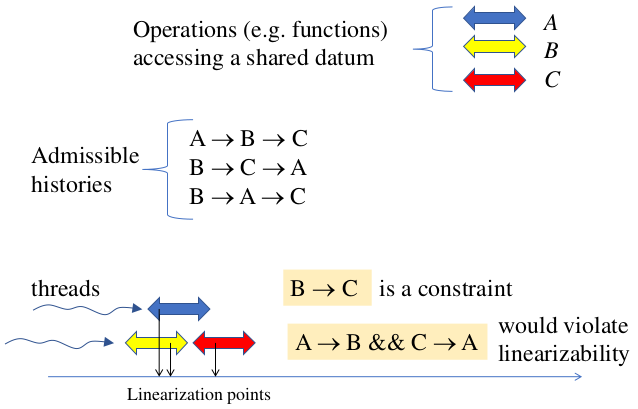
\includegraphics[scale=0.6]{immagini/wct.png}\\\\
Quindi, nella linearizzabilità, se due thread concorrono su una stessa struttura dati sarà visibile a gli altri threads mediante RMW quando qualcuno sta facendo operazioni sulla struttura dati, ma non sappiamo in che punto della timeline questo accadrà.\\ RMW permette che non accada niente altro nella specifica zona di memoria, in quanto come detto la linea di cache viene presa in uso esclusivo in MESI. \\ Possiamo avere due soluzioni differenti in algoritmi concorrenti:
\begin{itemize}
\item lock freedom: eseguiamo una operazione su qualche struttura condivisa, ma la RMW può fallire, anche la C\&S può fallire, perché magari l'operazione è andata in conflitto con quella di un altro thread che ha fatto qualche altra istruzione. Siamo in una situazione in cui non si è in grado di concludere l'esecuzione e quindi di rendere visibile agli altri la modifica. Nel caso lock free si ripete l'operazione, perché mentre sto lavorando io, qualcun altro ha già fatto qualcosa. La cosa interessante è che almeno un thread termina in un tempo finito, indipendente dalle attività degli altri: il numero di cicli di clock usati non dipende da lock o da cose dovute agli altri. Tutte le istanze terminano, con successo o no, in un tempo finito;
\item wait-freedom: tutte le istanze delle chiamate a funzione finiscono in maniera successfull, quindi non è possibile andare in abort. Questo magari perché le istruzioni non vanno mai in conflitto, quindi viene fatto sempre lavoro utile e non verrà mai determinato un abort
\end{itemize}
Gli algoritmi sono utili perché, per il fatto che tutte o alcune delle istanze portino avanti attività corrette, nessuno si aspetta: in un sistema moderno, sui thread che eseguono attività per toccare strutture dati condivise ci sono diversi vantaggi:
\begin{itemize}
\item crash sul thread, se si prende un lock ed il thread crasha è tutto bloccato
\item su un architettura moderna si lavora con VM: la VM fa girare l'algoritmo in maniera dedicata, se il thread che ha preso il lock viene deschedulato dal vero SO della macchina, quindi la vCPU viene deschedulata, si tiene il lock bloccato per molto tempo usando istruzioni macchina ed energy nei processori
\end{itemize}
Senza lock tutto ciò non avviene: se giro l'algoritmo sulla VM ed un thread viene deschedulato non ci sono problemi, gli altri thread della VM vanno avanti.\\ Gli aspetti fondamentali della lock freedom sono quindi che
\begin{itemize}
\item si può fallire, questo porta alla possibilità di ricominciare. Mentre se la RMW non fallisce, ovvero nell'algoritmo difficilmente si va in conflitto sulla stessa linea di cache, si completa senza fallimenti
\end{itemize}
\textbf{esempio: linked list non bloccante}\\
Abbiamo una linked list condivisa, vediamo l'inserimento condiviso: scandiamo la lista e troviamo l'elemento dove inserire, nessun altro sa che sto facendo un inserimento. Abbiamo letto il pointer dell'elemento che serve, quindi possiamo leggere in C\&S per aggiornare l'elemento, a seconda del fatto che la C\&S fallisca o no, capiamo se qualcuno ha aggiornato o meno quell'indirizzo.\\\\
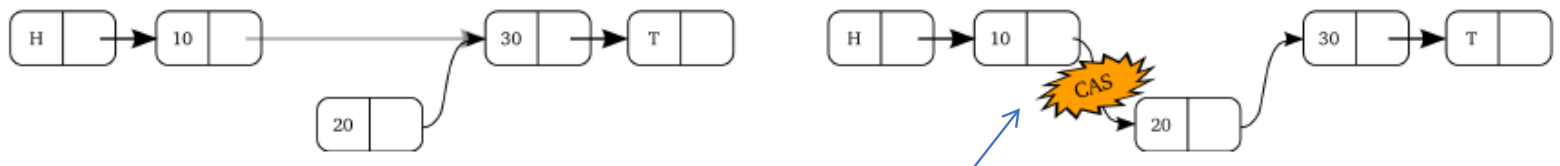
\includegraphics[scale=0.3]{immagini/cas_insert}
\\\\Leggermente più complesso è la remove di un nodo: non basta una C\&S, in quanto può accadere che un thread potrebbe inserire un elemento ed io voglia eliminare quello a cui il primo thread aggancia la sua insert. L'elemento va marcato con una C\&S come "da rimuovere", quindi ogni oggetto della lista avrà un pointer al successivo ed una bit mask che ne rappresentano lo stato\\\\
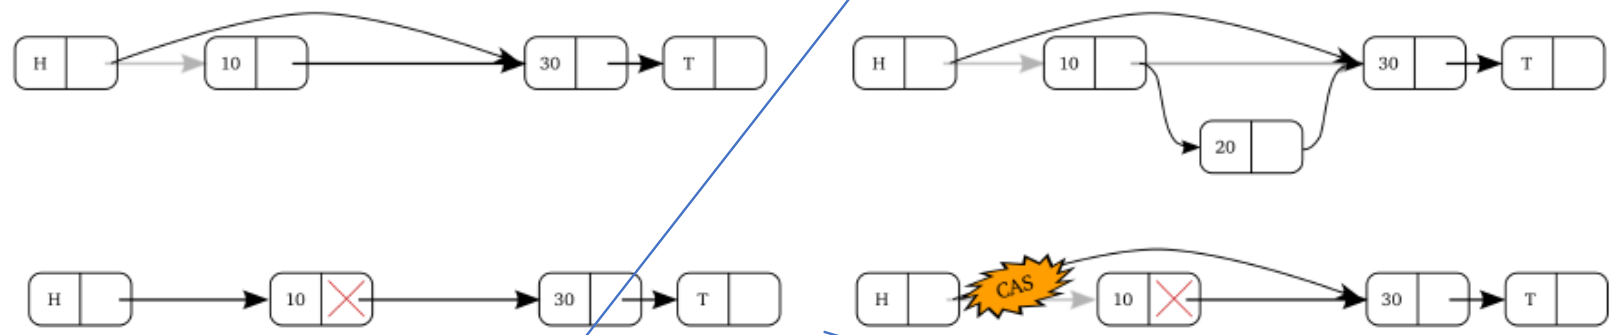
\includegraphics[scale=0.3]{immagini/cas_delete}\\\\
Supponiamo di avere dei thread concorrenti che fanno delle operazioni: un thread vuole rimuovere un elemento, lo marca e poi va in C\&S per eliminarlo (attaccare la head al successivo), sono due operazioni non atomiche. In un $\delta$ temporale un thread concorrente può attraversare la lista fino all'elemento che è marcato, che lo usa per lavorarci; nel mentre il thread che sta facendo l'eliminazione la completa e lo rilascia all'allocatore di memoria. Ma nel mentre qualcun altro può richiedere ed ottenere quella stessa area di memoria e scriverci delle informazioni. C'è quindi un problema di garbage collection dei nodi, occorre capire quando è effettivamente possibile rilasciare il nodo all'allocatore di memoria. Questo viene risolto da RCU, tecnica che non è bloccante solo per chi legge la struttura dati, mentre per chi aggiorna deve serializzare. Ma le strutture dati kernel sono molti lettori e pochi scrittori, quindi non ha senso bloccare la marea di lettori, si bloccano solo i pochi scrittori.\\ Un altro esempio è quello del \textbf{registro atomico}: abbiamo un'area di memoria m che è il registro, che è aggiornabile. Come aggiornarlo: o con locks, oppure con algoritmo apposito: implemento il registro come pointer, quando devo aggiornare il registro alloco una area appresso di m byte, in maniera atomica vado ad aggiornare  il pointer. Funziona solo se non c'è memory leakage, in letteratura è possibile implementarlo con al più n+2 slots, dove n sono reader ed uno è il writer. La soluzione è wait free: n+2 slot per leggere l'informazione, n possono essere concorrentemente letti, uno slot serve per tenere l'ultimo valore ed un altro per produrre un nuovo valore da pubblicare.\\ La soluzione si basa su avere all'interno dell'esecuzione dei thread una sola variabile di sincronizzazione, usabile in modo atomico tramite ISA (quindi RMW), abbiamo l'ultimo slot scritto e quanti reader hanno letto quello slot.\\ Per leggere, un thread preleva un indice ed in maniera atomica si marca come reader, lo scrittore può, da un altra parte, pubblicare un altro indice, 0 lettori e prelevare l'indice vecchio per vedere quanti lettori sono attestati su quello vecchio.\\ Ora negli slot è possibile capire quanti thread hanno finito di leggere e quanti stanno leggendo. Il reader dell'algoritmo fa una fetch\_\&add per prendere l'indice, ma la volta dopo confronta l'indice preso col valore presente nella variabile di sincronizzazione e se non è ancora cambiata si rilegge dallo stesso slot. Da un punto di vista delle performance, si ottengono dei risultati adeguate e che scalano molto bene. Di seguito, vengono mostrati gli pseudo-codici per l'implementazione del registro atomico:\\\\
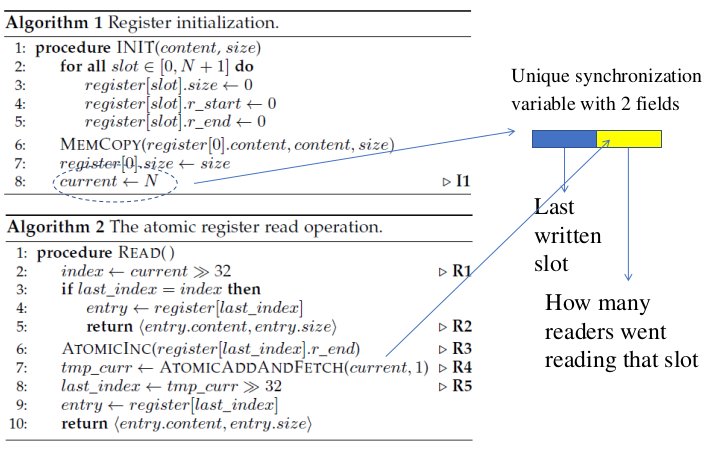
\includegraphics[scale=0.7]{immagini/atom_reg_1}\\
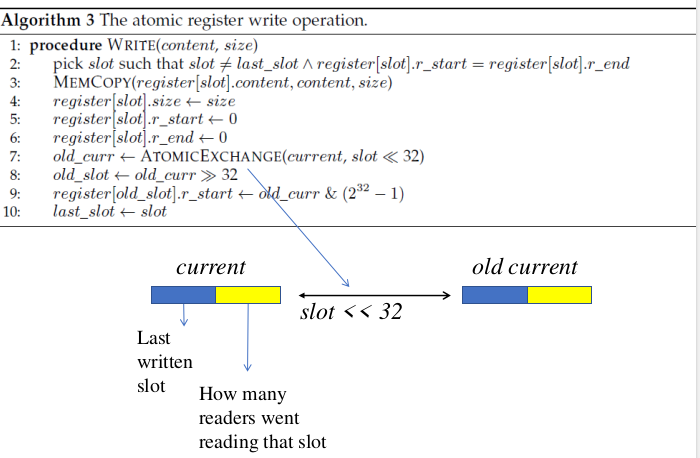
\includegraphics[scale=0.7]{immagini/atom_reg_2}\\
Gli approcci ci portano a capire che quando vogliamo un algoritmo concorrente e magari wait free, c'è una complessità maggiore del caso in cui stiamo lavorando con dei lock.
\section{Approccio di RCU}
È l'approccio alla base della costruzione di un sistema operativo moderno, ovvero che può girare su migliaia di CPU core dove i thread che sono in esecuzione condividono tutte le strutture dati.\\ La Read-Copy-Update permette di avere su una struttura dati condivisa un solo writer alla volta, quindi questi si sincronizzano fra di loro con dei lock, mentre i reader no. Questo favorisce delle strutture dati read-intensive che sono molte, una di queste è la hash table che mantiene quanti thread sono creati e quale è l'ID del thread.\\ La gestione dei collegamenti nella struttura dati è fatta nel seguente modo:
\begin{itemize}
\item gli outlinks della struttura dati che vengono rimosse logicamente, ad esempio come una remove di un nodo dalla lista collegata, non prevede al reale rimozione dei buffer ma vengono mantenuti attivi fino al \textbf{grace period}, ovvero periodo dopo il quale sono sicuro che chi sta attraversando la lista non lo fa pi attraverso il link che sto eliminando. Quindi ora l'aera di memoria può essere resa all'allocatore senza problemi
\end{itemize}
Il grace period su un SO reale viene implementato in maniera semplice, e questo si può fare anche a livello user e quindi RCU è uno schema che si può usare sia a livello kernel che a livello user per avere strutture dati scalabili in termini di accessi.\\ Abbiamo quindi il concetto di \textbf{standing readers}, che possono continuare ad usare aree di memoria rimosse, fino a che non avranno terminato l'esecuzione. Di seguito, viene mostrata la classica timeline di RCU
%immagine della timeline
i reader sono pienamente concorrenti al writer, quindi può accadere che la fine dell'esecuzione di alcuni dei reader va considerata dal writer prima della riconsegna dell'area di memoria, può anche capitare che un reader cominci a leggere dentro il grace period, quindi già con lo snapshot della struttura dati aggiornata%quindi il grace period può essere esteso se necessario
Vediamo come implementare lo schema, quindi come capire quando i reader iniziano e finiscono le operazioni rispetto a quando sta operando il writer: i concetti di base sono i seguenti\\
Il reader
\begin{itemize}
\item deve segnalare che c'è
\item deve leggere
\item deve segnalare che non c'è più, perché ha finito
\end{itemize}
Il writer
\begin{itemize}
\item prede il write lock
\item gestisce l'update della struttura dati, rimuovendo delle cose per generare un nuovo shape della struttura dati
\item attende i reader standing
\item i reader che si segnalano come presenti sulla struttura aggiornata vengono linearizzati dopo il writer
\item release del buffer
\end{itemize}
Vediamo ora come effettivamente vengono implementate le cose
\subsection{Kernel level RCU}
A livello kernel, è possibile per un execution flow disabilitare la preemption e riabilitarla: il CPU core non può essere ceduto ad un altro execution flow finché non è deciso, eseguire e poi tornare preemptable. Quindi, se nella fase non-preemptable si esegue una RCU, abbiamo un buon modo per poter leggere la struttura: disabilitando, si segnala di leggere, abilitando si dice di aver finito; in questo modo nessun altro può avere il CPU core\\ il writer prende il lock, aggiorna la struttura dati ed alla fine deve chiedersi se c'è ancora qualche reader da linearizzare prima che il buffer venga de-allocato. Dopo aver finito quindi gira su tutte le CPU, ovvero chiamando servizi kernel per eseguire sulle diverse CPU e sarà possibile ottenere le CPU solo quando queste verranno rilasciate dai reader. Il problema è che questo avviene quando il numero di CPU core non è così elevato da permettere questo aggiornamento. La linea di codice per girare su tutte le CPU è la seguente: \textsf{for\_each\_online\_cpu(cpu) run\_on(cpu);}\\ Vediamo come fare senza abilitare/disabilitare le preemption
\subsection{Preemptable RCU}
Le RCU devono essere preemptable, quindi il thread può perdere la CPU, usiamo un concetto classico e relativo all'epoca: se appartengono all'epoca vecchia della struttura, occorre aspettare che l'epoca finisce; se invece sono tutti nella nuova epoca il writer non deve attendere.\\ Andiamo a ragionare sull'atomicità di cosa si può fare , in particolare è possibile aggiornare un contatore in maniera atomica, che sarà un \textbf{presence counter}, ovvero che indica la presenza nell'epoca. Quando il writer aggiorna la struttura dati, deve farla transitare nella nuova epoca e si ottiene con la ridirezione dei reader su un altro counter: un puntatore sa quanti reader stanno leggendo la struttura, si aggiorna la struttura e poi si aggiorna il puntatore al contatore successivo. C'è il rischio di dover aspettare un reader che sta già osservando la nuova shape, ma che ancora non rilascia il contatore vecchio, questa può essere la timeline della situazione:
%immagine della timeline
Se uno dei thread crasha, può non essere in grado di decrementare il contatore, vuol dire che i buffer non possono essere lasciati all'allocatore ma non ci sono blocchi, la struttura può comunque essere rilasciata, è possibile comunque introdurre dei TO per sincronizzare il tutto.
\section{Aspetti ulteriori di parallelismo}
Abbiamo parlato più volte di parallelismo, abbiamo anche altri aspetti di parallelismo sul processore che è il concetto di 1\textbf{vettorizzazione}: possiamo eseguire delle istruzioni secondo la forma del processamento SIMD (Single Instruction Multiple Data); ci sono anche altri paradigmi come MIMD, che è a disposizione sui multi-processori o multi-core.\\ SIMD è basata sul concetto dei \textbf{registri vettoriali}, quindi registri che contengono diversi slot a 32/64 bit, quindi l'istruzione in maniera automatica sta già usando la vettorizzazione. SIDM è presente nei processori moderni, anche ad esempio nella GPU che è tipicamente SIMD, che specializza questo concetto. \\ Un altro aspetto interessante è la MISD (Multiple Instruction Single Data): due istruzioni sono su un flusso, che è un thread, due istruzioni scrivono su un registro in parallelo ed è possibile farlo in parallelo perché su architetture speculative si scrive su un renamed register.\\ Abbiamo infine SISD, che è il triviale (slides)
\subsection{Vettorizzazione su x86}
I processori sono fatti in modo che per le istruzioni SIMD, nell'architettura l'esecuzione si basa su l'uso di hardware "apposito", es. sommatori vettoriali per fare delle sommatorie che hanno più dati in input e forniscono più output. Lo schema astratto è il seguente:
%immagine
Su x86 il supporto per l'esecuzione vettorizzata è \textbf{SSE} (\textbf{SSE-2} in 64 bit): abbiamo 8 registri vettoriali a 128 bit, dove possiamo mettere un vettore di informazioni. In SSE possiamo quindi inserire diverse combinazioni di valori
%immagine
con l'estensione AVX i registri sono raddoppiati in numero e possono essere usati per due lane differenti
%immagine
\subsection{Allineamento della memoria}
Alcune delle operazioni che portano dati nei registri lo fanno in maniera corretta solo se l'indirizzo è allineato a certi vincoli, possono esserci vincoli di allineamento ad 8 o 16 byte e questo è importante perché se viene chiamato un intrinsic di gcc che usa una di queste istruzioni può essere necessario avere allineamento di memoria. Abbiamo visto che è possibile in C avere aree di memoria già allineate (vedi istruzioni sopra).\\ Ci sono diversi instrinsics gcc da chiamare per poter usare i registri vettorizzati:
%immagine degli instrinsics
\section*{RCU list, note di implementazione}
\begin{itemize}
\item la struct \_rcu\_list viene creata con typedef \textbf{packed}, che fa si che il compilatore non apporti delle modifiche come padding etc... Quindi, viene generato un eseguibile generato con lo stesso numero di bytes del sorgente in termini dei dati, perché magari vogliamo gli oggetti allineati a 64 byte, o magari perché abbiamo scelto di inserire i diversi campi della struct in diverse cache lines;
\item La bitmask serve per definire, in base al valore dell'ultimo bit, in che epoca siamo: la variabile indica sia un contatore e sia l'epoca;
\item abbiamo due epoche, past e current, ma si può ampliare per transitare nelle diverse epoche in base ai readers presenti;
\item nella insert, si fanno mfence in quanto quello che accade è che non vengono esclusi i lettori: se sposto la head e lo faccio puntare ad un nuovo elemento e gli updates non sono resi pubblici a livello dell'ISA, si rischia di rendere visibili degli updates non corretti;
\item anche nel caso della remove, la mfence serve per evitare che i readers che nel mentre leggono, vedano dei valori non consistenti dovuti ad un aggiornamento non ancora propagato;
\item \_\_atomic\_exchange\_n(), gcc intrinsic;
\item il reader esegue fetch\&add di continuo, uscendo ed entrando nell'epoca, passando come parametri l'epoca. L'add aggiunge sempre una unità, questo va bene se la locazione è in grado di acquisire l'aggiunta, quindi la variabile che implementa il meccanismo di sincronizzazione basica va in overflow, deve esserci quindi un meccanismo che porta il valore a 0. \textbf{Thread house keeper}, che si occupa di mettere a posto le cose: prende uno spin lock come se facesse un aggiornamento, ma fa solo un cambiamento dell'epoca (quindi da 0 ad 1 o da 1 a 0 nel caso dell'esempio) e si aspetta che i reader che sono nell'epoca precedente finiscano. Serve per ri-sincronizzare le poche e riportare le strutture dati allo stato corretto;
\end{itemize}
Quale è infine, lo svantaggio del fatto di avere una soluzione preemptible piuttosto che non preemptible? Nel caso non preemptible, non rispettiamo le priorità: se c'è un thread ad alta priorità che deve eseguire ed è pronto ad eseguire, con uno schema di questo tipo non siamo fair e non permettiamo al thread di andare in esecuzione, che può diventare un problema nel caso in cui la sezione critica ha una lunga esecuzione.
\chapter{Kernel programming basics}
\section{Addressing}
\subsection{Linear addressing}
Vediamo le modalità con cui si fa addressing di dati ed istruzioni. Una delle modalità più interessanti che ci sono è il linear addressing, in cui le informazioni usabili dal processore sono viste come una sequenza lineare, quando esprimiamo un indirizzo l'unica cosa da specificare è un offset, ovvero il punto dove collocarsi con l'operazione di lettura/scrittura. L'indirizzamento è di memoria, magari anche di memoria fisica, oppure di memoria logica, per cui distingueremo indirizzamento fisico e logico.\\ Quello che realmente accade in architetture moderne e che si usano anche altri concetti, tra cui la segmentazione
\subsection{Segmentazione}
Abbiamo un address space in cui il processore può leggere/scrivere. Potremmo identificare delle zone differenti, che sono magari indirizzabili non solo tramite offset, ma esprimendo un segment\_id + offset, quindi l'offset è interno allo specifico segmento. In un sistema moderno si combinano i due approcci: si dice che si vuole accedere ad un segmento specifico, ma poi l'accesso al singolo segmento viene tradotto come offset in una zona lineare: quindi possiamo avere questo tipo di collocazione:
%immagine
l'accesso a B va tradotto nel calcolo assoluto dell'offset all'interno dell'address space lineare. Il punto nodale è che quando esprimiamo un indirizzo per toccare delle informazioni, questo passa per la nozione della base del segmento a cui si vuole accedere, perché l'indirizzo sarà dato dalla base + l'offset a cui si vuole accedere. Ricordiamo che la memoria può essere sia fisica che logica, quindi abbiamo o non abbiamo il passaggio in più, legato al concetto di memoria virtuale
\subsection{Memoria virtuale}
(slides per immagini ed altro)
Se siamo in memoria logica, vogliamo prendere un indirizzo lineare ed accedere alla zona di memoria, ma non sappiamo se è in memoria e dove è in memoria fisica. Quindi il passaggio in più è presente o meno a seconda dell'hardware e del software che si utilizza.\\ In ogni caso, quello che il processore deve fare è: indirizzo segmentato $\rightarrow$ indirizzo lineare $\rightarrow$ indirizzo nella pagina $\rightarrow$ indirizzo fisico. Abbiamo supporto per eseguire la traduzione e la traslazione degli indirizzi in maniera efficiente, e questo vuol dire anche capire se l'accesso ni memoria che si sta cerando di risolvere è plausibile in quel momento o no, in termini dei privilegi che il processore ha in quel momento. Esempio in x86:
\textsf{mov (\%rax), \%rbx}, \textsf{push \%rbx}, qui stiamo usando 3 segmenti differenti, non li usa chi ha scritto il programma, bensì il processore in maniera autonoma si rende conto che le operazioni stanno toccando diverse zone di memoria: i due segmenti sono dati dagli indirizzi di \%rax, dal fatto che si fa la push di \%rbx, il terzo è dato da dove sono le istruzioni. Il processore sta eseguendo il fetch delle istruzioni, che è un accesso in memoria e quindi passa tramite le regole dette sopra.
\subsection{Processori di sistema e segmentazione}
I processori di sistema sono quelli per cui pensiamo di eseguire codice di SO, qui il supporto per eseguire la traslazione e validarli è dato da un'insieme di informazioni tipicamente mantenuti in un insieme di registri o tabelle di memoria, il che vuol dire che oltre alla page table servono anche altre informazioni per accedere alla memoria che sono interni ad altri componenti e sono:
\begin{itemize}
\item registri di CPU
\item Tabelle in memoria, puntate direttamente dai registri
\end{itemize}
Sui processori moderni ci si muove sia con la segmentazione che con gli indirizzi lineari, quindi si esprime un indirizzo segmentato che viene traslato in lineare etc... come sopra, quindi tutti i passaggi hanno bisogno delle informazioni che vengono inserite in registri e tabelle: tipicamente lavoriamo con la page table, per cui se abbiamo un indirizzo lineare, possiamo paginarlo ed associarli un indirizzo fisico. Per avere una traslazione di indirizzo segmentato a lineare possiamo avere la seguente traduzione in hadware:
%immagine slides.
\\ Consideriamo qualcosa in più,s il concetto del segment selector
\subsubsection{Segment selector}
Quando si usa un indirizzo segmentato, viene specificato il registro del segemtn selector, quindi non il nome del registro bensì il nome del registro. Il registro contiene le informazioni sul segmento che si vuole prendere, quindi abbiamo il seguente schema:
%schema
se abbiamo una istruzione macchina per accedere ad uno specifico segmento in memoria, per poi in futuro accedere ad un altro, è possibile usare sempre la stessa istruzione e basta specificare il registro di segmentazione corretto. Il caso classico è se il codice viene eseguito su un thread piuttosto che un altro, il codice macchina è identico, che però tocca segmenti differenti usando questo tipo di meccanismo.
\section{Accesso in memoria su x86}
Abbiamo il real mode x86, un po' datato, il real mode ed il long mode (variante più recente). Vediamo l'x86 real mode 
\begin{itemize}
\item segment register a 16 bit, ce ne sono 4
\item registri a 16 bit generali per gli offset. Possiamo specificare in una istruzione dove specifichiamo di accedere alla memoria dove punta quel registro, che può essere un puntatore
\end{itemize}
L'indirizzo fisico a cui accediamo è calcolato come: \textsc{Segment}*16+\textsc{Offset}. Possiamo accedere a circa 1 MB di memoria, la cosa interessante è che nei registri non si mantenevano informazioni riguardo alla protezione, quindi la macchina non era adeguata per implementare software di sistema, perché non c'è la nozione di protezione, quindi nemmeno software relativo alla VM. Tutto ciò che esegue può usare questo schema.
\subsection{x86 protected mode}
Abbiamo le seguenti caratteristiche:
\begin{itemize}
\item registri a 16 bit per tenere i segment ID, usiamo solo 13 bit per specificare gli ID, con gli altri specifichiamo delle caratteristiche relative ai privilegi: un certo segmento può essere toccabile solo se si lavora ad un certo livello
\item registri general purpose a 32 bit, usati come pointer e che puntano nel segmento 
\end{itemize}
quando vogliamo toccare un certo segmento, ci chiediamo quale è la base nell'indirizzamento collocato e quale è il suo offset: l'ID del segmento nel registro segmentato è un indice della tabella, che contiene la base del segmento e quindi avremo che gli indirizzi che otteniamo sono lineari: \textsc{address} = \textsc{TABLE[segment].base + offset}. Possiamo quindi identificare l'offset assoluto nella memoria per poter leggere e scrivere, essendo i registri di offset a 32 bit, possiamo indicizzare 4GB. I 3 bit non usati possono essere impiegati per la protezione, quindi l'istruzione permette di toccare determinate zone di memoria in base alle determinate configurazioni
\subsection{x65 protected mode}
È una estensione del precedente
\begin{itemize}
\item segment registers a 16 bit, di cui ne usiamo sempre 13
\item registri general purpose a 64 bit per usare gli offset per accedere in memoria. Se usiamo lo stesso meccanismo di prima, è tutto a 64 bit e quindi avere $2^{64}$ come offset bello spazio lineare. Ma non è così, abbiamo solo 48 bit disponibili: preso un registro come \textsf{rax}, mettiamo una bitmask che esprime un offset per accedere alla memoria, possiamo scrivere i 64 bit come vogliamo, ma quando passiamo questo all'interfaccia per l'accesso alla memoria, vengono scartati i bit in più e se ne usano solo 48 (gli altri sono settati a valori di defualt)
\end{itemize}
Qui possiamo indicizzare 256 TB di memoria, quindi di indirizzi di memoria.
\subsection{Tabella di segmentazione}
In x86, quando abbiamo un segment selector, abbiamo un ID e le tabelle considerate possono essere 2 per ogni flusso di esecuzione
\begin{itemize}
\item GTD
\item LDT
\end{itemize}
possiamo specificare se l'indice è riferita all'una o l'altra tabella, mediante l'utilizzo di un apposito bit di controllo che specifica quale tabella considerare. In sistemi moderni, si considera solo la GDT, che ad ogni istante di tempo dice, dato un thread in esercizio sulla CPU, esattamente ogni segmento toccabile dai selettori dei registri usati dal thread. La GDT indicava qualcosa di globale, nel senso che venivano indicate anche informazioni riguardo la base del segmento accessibile a livello kernel, ma questa informazione valeva per tutti i thread. La struttura della GDT è la seguente
%immagine GDT
in una entry, oltre alla base del segmento, ci sono anche flags addizionali per gestire correttamente il segmento. Sappiamo come accedere al segmento, i flags specificano cosa si può fare con quel segmento.
\subsection{Segmentazione e paginazione}
Nella GDT ci sono informazioni per la gestione del segmento, ma da un indirizzo lineare si passa ad uno fisico e c'è la tabella delle pagine che ha anche essa dei bit di protezione, sappiamo se il frame che tocchiamo è di livello kernel o user. Quindi perché c'è questo overload nel meccanismo di protezione, inoltre perché è presente anche la segmentazione nonostante la paginazione gestisce la memoria. La paginazione è un modo per gestire la memoria a grana molto fine, mentre la segmentazione è a grana molto più grande: potremmo avere un address space lineare fatto da un unico segmento $s_0$, quindi la protezione per il segmento è per l'intero address space, diverso da quelle che potrei avere per le singole pagine nella page table.\\ Inoltre, l'architettura per cui abbiamo la segmentazione per accedere alla memoria è stata estesa perché con la segmentazione data una istruzione macchina correntemente in esecuzione sulla CPU, è possibile che il thread ad un certo istante di tempo tocca lo spazio lineare da una certa parte, mentre l'istruzione per un altro thread tocca l'address space lineare da un'altra parte. I thread possono girare su diverse CPU se abbiamo TLP, quindi eseguire delle istruzioni macchina identiche ma toccando diverse zone di memoria, quindi possiamo gestire la memoria segmentata in maniera più modulare di come faremmo con la paginazione, quindi è la base del multi-threading e del multi-coring:
\begin{itemize}
\item Thread Local Storage
\item Per-CPU memory
\end{itemize}
Nella segmentazione, la grana di protezione è più grossa in quanto con pochi bit si può andare a definire cosa fare anche su un intera area di memoria, ma è utile sopratutto quando si lavora con TLP, quindi in maniera concorrente, inoltre la segmentazione è stata portata avanti quando la paginazione era già supportata dai sistemi.\\ Scendiamo nel dettaglio della protezione della segmentazione
\subsection{Protezione nella segmentazione}
Possiamo associare a ciascun segmento un certo livello di protezione, o livello di protezione. Ragioniamo sulle variazioni di flusso di esecuzione, ma gli stessi concetti valgono anche per l'accesso ai dati, ogni routine che ha un livello di protezione h in uno schema di protezione basato su segmentazione può invocare qualunque altra routine, che può essere anche in un altro segmento, di livello h. Quindi, i salti possono essere intra-segment ma anche cross-segment, ma occorre che il livello di protezione della sorgente e del target siano allo stesso livello di protezione. Possiamo anche muoverci con valori differenti di protezione, dobbiamo sicuramente avere un salto cross-segment, perché se fossimo nello stesso segmento si avrebbe lo stesso livello, è sempre possibile saltare al livello h+i, se questo è il livello target, si passa ad una routine meno privilegiata.
\subsubsection{Protection GATEs} 
Abbiamo che ogni segmento ad un livello di protezione h è  associato con un insieme di access points, detti \textbf{GATEs}, ognuno identificato con una coppia $<$seg.id,offset$>$ ed ogni GATE ha associati un livello massimo max = h+j da cui è possibile saltare.\\ Quindi il passaggio a livello superiore si può fare solo se la prima istruzione macchina della routine è un così detto GATE di accesso. Passare per il GATE vuol dire che non si possono usare le stesse istruzioni macchina che si eseguivano per saltare nello stesso segmento, i GATE sono porte di accesso che permettono di "entrare e diventare più privilegiato", ma non è ammesso a qualunque thread, bensì ad un massimo livello di privilegio ammissibile per passare nel GATE.\\ Quindi, se il livello di S è h, ed il max(GATE(S)) = h+i, allora il segmento S ha un GATE che permette l'accesso ai moduli che hanno un livello di protezione da h+i in su. Il modello basato su segmentazione implementa un \textbf{ring model}:
%immagine del primo ring
eventualmente si salta da 0 in avanti in dei target che hanno dei livelli di protezione peggiori o pari a chi salta, mentre per fare il contrario dipende dal GATE. Abbiamo quindi un address space lineare, fatto da zone che sono dei segmenti e possiamo avere segmenti livello user o kernel:
%immagine dei segment
abbiamo 3 routine, una user e due kernel, le due istruzioni kernel sono GATE:
\begin{itemize}
\item nel GATE kernel routine A si permette il passaggio solo intra-segment;
\item il GATE kernel routine B ha un max pari a 3, quindi ad esempio provenendo dal GATE del livello S2 si può saltare nel segmento a livello di privilegio B, ed a quel punto chiamare il GATE di A
\end{itemize}
Possiamo perciò comporre in un address space non solo il meccanismo della paginazione, che ci dice che i segmenti sono kernel, ma la segmentazione offre supporto in più per avere questo passaggio che permette di usare davvero quello che è presente nel segmento kernel.\\ Quindi gli obiettivi della segmentazione sono offrire delle protezioni ulteriori rispetto a quelli della paginazione, inoltre permette di cominciare a fare qualcosa in un livello di protezione maggiore: in uno SO abbiamo un interrupt, magari mentre eseguiamo software di livello user ad un certo istante t, per processare le attività associate all'interrupt che sono magari cablate in attività lato kernel, occorre passare a privilegi lato kernel; quindi, per ogni interrupt deve essere definito un GATE, altrimenti non è possibile gestire l'interrupt.\\ 
(((Quando viene chiamata una syscall abbiamo un oggetto machine-dependent del tutto generale chiamato dispatcher, in grado in funzione del fatto che è stata chiamata una syscall e quindi una trap, di leggere il valore eventualmente scritto in un registro e capire dove redirigere il flusso di esecuzione nel codice kernel.)))\\Abbiamo quindi interrupt e GATEs, con cui permettiamo a software di livello user di eseguire attività necessarie.
\subsection{Ring model in x86}
Lo schema ad anello dell'x86 è fatto nel seguente modo:
%immagine del ring
servono quindi, per discriminare il livello di protezione 4 bit in quanto abbiamo 4 livelli diversi di protezione. A livello 0, all'interno di una architettura segmentata abbiamo tutte le informazioni del kernel: possiamo fare qualsiasi cosa, ovvero toccare qualsiasi altra informazione anche a livello user.\\ Tipicamente le applicazioni user girano a livello 3, i due livelli intermedi inizialmente non erano nemmeno usati, man mano sono stati usati per implementare servizi di sistema, ad esempio per la schedulazione delle VM.\\ Quando facciamo qualsiasi accesso in memoria, si va a specificare il segment seletor register ed eventualmente un displacement, in modo che riprogrammando il registro per attività in tempi differenti, andremo in diverse aree di memoria. Vediamo quanti e quali selettori di segmenti ci sono
\subsubsection{Registri di segmento}
Il registro di segmento ha informazioni sia sul nome del segmento, sia informazioni sulla protezione del segmento (16: 13 $|$ 3).\\ Su x86 l'utilizzo comune prevede solo la GDT, ma c'è comunque un bit che dice dove andare a prendere il segmento, abbiamo poi altre informazioni di protezione. I selettori di segmento sono 6, i primi 4 erano quelli originali e gli altri due sono stati aggiunti, quindi la segmentazione è andata avanti a prescindere dalla paginazione
\begin{itemize}
\item CS: si stabilisce in un address space quale è la zona dove è presente il codice di cui fare i fetch. Discriminiamo cosa è usabile dal punto di vista di esecuzione del processore, il registro viene ad esempio usato proprio dal processore quando deve andare all'istruzione successiva
\item SS: in che zona dell'address space è posizionata la zona di stack. Viene usato quando si fanno push e pop
\item DS ed ES: segmenti dati, usabili per accedere ai dati delimitandone la posizione nel segmento specifico
\item FS e GS: aggiunti dopo
\end{itemize}
Quando lavoriamo su CS, i 2 bit RPL sono anche detti CPL ovveo il Current Priviledge Level, quindi quale è la capability del processo in esecuzione.\\ Analizziamo uno snippet visto in precedenza, possiamo capire quali sono i registri di segmento usati:
%snippet
Abbiamo un offset all'interno del code segment, perché usiamo il PC per fetchare le istruzioni che è un offset, la base è dato dal CS. Il DS è un offset per accedere alla memoria, il pointer di default dice dove acquisire il dato. La push utilizza l'offset per capire dove andare in memoria, quindi usa il registro SS. ES viene usato al posto di DS quando si eseguono delle istruzioni particolari, ad esempio quelle string-targeted come \textsf{stos} e \textsf{movs}
\subsection{GDT di x86}
La tabella fondamentale che contiene le informazioni sul fatto che dato che qualcuno sta facendo una istruzione che deve fare qualcosa, dice quel qualcosa dove è in memoria. Questa è una entry della tabella:
%immagine
ciascuna entry da informazioni sul segmento associato a quell'indice. La tabella è fondamentale, perché il registro può essere cambiato e quindi anche l'informazione per il segmento di indice i va salvato, altrimenti non saprei come recuperarne le informazioni.\\ La tabella ha 8 byte usabili per un processore ad 32 bit, manteniamo
\begin{itemize}
\item base 0:15
\item base 24:31
\item base 16:23
\end{itemize}
tutte le altre informazioni sono di controllo
\begin{itemize}
\item access byte: dice se la entry è valida o no
\item limite, dice al  più quanto è ampio il segmento, quindi quale è il massimo offset per accedere, può avere diverse taglie (in base al valore limit 16:19???)
\end{itemize}
Il privilege level viene caricato in un registro di processore quando vogliamo usare un segmento nel programma.
\subsubsection{Accesso alla GDT}
Se vogliamo accedere ad un segmento e caricare le informazioni su quel segmento, come fa il processore a sapere dove è in memoria quel segmento: c'è un registro apposito che è il \textbf{gdtr}, puntatore che porta all'interno della memoria per sapere dove è posizionata la GDT. È un puntatore, quindi un offset ma rispetto a quale memoria? Stiamo cerando di identificare nella memoria alcune informazioni basiche per gestire la memoria segmentata, quindi è in memoria lineare. L'organizzazione è la seguente:
%immagine dell'organizzazione
È interessante che gdtr si può leggere anche a livello di privilegio 3, magari non si riesce ad accedere a quel punto della memoria, perché magari è in un segmento non accessibile a livello 3.\\ Quando leggiamo il registro, in realtà abbiamo una informazione packed
\begin{itemize}
\item l'indirizzo del registro
\item il numero di entry che la tabella ha correntemente
\end{itemize}
mettiamo le informazioni in una struttura packed, usando la API \textsf{store\_gdt}, che è codice asm volatile che non fa altro che prendere sgdt e mette il valore nel puntatore. La chiamiamo due volte, passando due parametri differenti, in un caso un array di byte.
%snippet di codice
dalla comparare il valore dei puntatori: è possibile, anche se con scarsa probabilità, che abbiano diversi valori, ma la si può aumentare chiamando un servizio bloccante come la sleep\\ Se l'applicazione venisse schedulata e poi reschedulata su un'altra CPU, avremmo trovato dei valori di GDT differenti\\\\ A 64 bit abbiamo che la taglia delle entry è il doppio,  manteniamo alcune informazioni 
%immagine della entry a 64 bit
Supponiamo di voler usare un selettore di segmento, avendo anche l'indice, sarebbe importante sapere l'offset del segmento perché altrimenti non potremmo fare tutti gli altri passaggi. Sappiamo che è nella GDT, accediamo con un selettore di segmento, accediamo ad un offset, viene  mostrato in seguito uno schema
%schema della somma e dell'accesso
Su x86, quando abbiamo un segment selector, invece di andare sempre in memoria l'informazione viene cachata in una zona apposita quando abbiamo già il selettore, l'aggiornamento di un selettore prevede che si vada in tabella, si prenda il selettore e si metta l'informazione in una cache interna al processore\\\\
\textbf{esempio software, va risentito da una rec con video sennò è impossibile capire penso}\\
Quello che capiamo è che andando a toccare i diversi segmenti, questi possono essere mappati sullo stesso segmento.
\subsection{Code e data segment per Linux}
Vediamo come Linux configura la GDT usata da uno dei processori per capire dove sono posizionati i segmenti: ci sono 4 entry nella GDT usate da Linux
%immagine della tabellina
\begin{itemize}
\item user code: la entry tiene traccia di qual è la posizione del segmento dove ci sono istruzioni utente, la base è 0
\item user data: la posizione ha sempre base 0, quindi se usiamo un offset usando questo segmento o quello precedente arriviamo nella stessa area di memoria
\item kernel code: le informazioni che costituiscono la parte eseguibile del kernel è sempre a partire da base 0
\item kernel data: base 0 anche per lui
\end{itemize}
Se ragioniamo su cosa realmente accade, è che presi questi 4 segmenti di base, all'interno dell'address space questi sono sovrapposti, partono tutti dalla stessa base 0. Se abbiamo un offset per identificare un dato o una istruzione, in realtà questo è un offset assoluto, si identifica in maniera univoca una posizione nell'address space. La segmentazione resta fondamentale quando vanno gestiti i GATE, altrimenti non potremmo stabilire se, indipendentemente da come il processore raggiunge le cose nell'address space.\\ La scelta di usare al minimo la segmentazione nello sviluppo del kernel Linux: abbiamo un insieme di moduli che rappresentano il kernel Linux, la scelta di mappare a 0 tutti i 4 segmenti nativi è che, se supponiamo che i concetti di segmentazione sono spari ovunque nel kernel, quindi prendere il kernel e ridisegnarlo per portarlo su una macchina dove la segmentazione non c'è vuol dire riscrivere un kernel diverso. Altra cosa è se la segmentazione viene configurata in modo che l'offset è assoluto, viene ridotto l'impatto della segmentazione alle poche parti segmentation dependent, in modo da far si che è semplice portare il kernel per eseguirlo su macchine che usano la segmentazione. Ma se bisogna riscrivere il TLS in una architettura dove la segmentazione non c'è, va riscritto poco codice perché quello già esistente è molto portabile.
\subsubsection{Versione a 64 bit, long mode}
Nel long mode, ovvero x86\_64, i vendor hanno fatto sì che per tenere traccia del segment ID, per alcuni selettori di segmento la base è per default settata a 0, quindi l'offset è assoluto.\\ Per 4 dei selettori vale questo, per gli altri 2 vale ancora che la base associata al segmento va presa dalla tabella. Quindi per alcuni selettori si può accedere direttamente senza passare per la tabella, ma non per tutti altrimenti si perde la capacità di poter costruire software sfruttando la segmentazione, comunque questa scelta permette di accedere rapidamente ai segmenti discriminando solo aspetti di protezione, ma anche poter usare dei segment selector che vanno in due zone diverse nello stesso flusso di esecuzione.
\subsection{Gestione dei selettori in x86}
Se i segmenti non servono più a discriminare dove lavoriamo, perché sono tutti mappati a 0, il code segmenti rimane importante perché c'è il CPL: se è targato con CLP = 00, stiamo lavorando in qualche segmento di codice a livello kernel, se è 11 stiamo lavorando in qualche segmento ma non è vero che tutti è permesso. Questo ci mette già di fronte all'idea che una stessa istruzione macchina dell'ISA vine eseguita in diversi casi di valori di CPL possiamo avere diversi risultati, quindi il CPL al di là di dove sono posizionate le cose in memori permette di distinguere diverse modalità operative.\\ È possibile aggiornare CS? No, l'unico modo il cambiamento del CPL (se siamo su x86\_64 conta solo questo) avviene solo quando abbiamo dei control flow particolari. Una delle cause per generare queste conseguenze è il passaggio per un GATE, l'istruzione che fa passare nel GATE aggiorna il CPL, ovviamente quando CPL=0 p tutto lecito.\\ Tutti gli altri selettori di segmento possono essere aggiornati se il segment descriptor a cui sono associati ha DPL $\geq$ CPL corrente
\subsection{GDT estesa in Linux}
La GDT classica di Linux è la seguente:
%immagine
alcune entry indicano dove in una address space lineare vengono posizionati i dati kernel/user, ma gli offset che ci dicono dove sono posizionati i segmenti portano sempre a 0, quindi l'offset è assoluto. La segmentazione gioca un ruolo solo nei termini della protezione, vediamo inoltre che tra i segmenti interessanti c'è il \textbf{TSS}: è un segmento posizionato nell'address space a base diversa da 0 e se consideriamo un address space lineare abbiamo che data l'esistenza sulla macchina della CPU x, c'è una zona associata alla specifica CPU x, stesso vale per le altre CPU. I TSS sono queste zone "riservate", quindi esiste un segmento nell'address space lineare posizionato ad una base differente per ogni CPU (o hyperthread fisico).\\ Nel TSS ci sono informazioni basiche per tenere traccia, mentre su una certa CPU che esegue uno specifico thread, le cose relative al ring model, quindi come l'oggetto si muove nel ring model.
\subsection{TSS}
Il TSS era tale per cui l'oggetto era una collezione di informazioni, raggruppati in un array ed ogni array aveva un'associazione con lo specifico CPU core. Questo array aveva una certa taglia, un certo valore dei bit di protezione, è quindi un informazione accessibile a livello kernel, TSS da lo stato del task in esercizio sulla CPU. Internamente, su x86 ad esempio, abbiamo la seguente struttura:
%immagine della struttura
salendo nelle informazioni, troviamo locazioni di memoria che tengono traccia dei registri del processore. Potremmo installare nella zona uno snapshot del processore, ma anche informazioni di segmentazione che il processore sta usando, quindi tutta la fotografia del processore.\\ Inizialmente, era stato pensato per implementare il context switch a livello hardware, quindi con apposite istruzioni macchina.\\ Le zone ESP sono Extended Stack Pointer, quindi registriamo 3 stack pointers differenti, ma il processore ha un solo ESP: i 3 diversi stack poninter servono per avere nella specifica zona quali sono le capability del thread in ring model, così che sappiamo che se cambia il livello di privilegio, magari dobbiamo usare una stack area differente. La struttura viene usata anche dal firmware, il ring model = utilizzo eventualmente i GATE, quindi istruzioni macchina per cui il processore potrebbe dover cambiare priorità. Tutta la parte sopra è inutile, perché l'oggetto non è usato per implementare context switch hardware, su Linux è basato su software e quindi la zona sotto è stata espansa per ospitare stack pointer a 64 bit e poter avere nell'area una rappresentazione corretta delle informazioni che rappresentano il ring model. Quando arriva un interrupt, ed il thread che esegue deve cominciare ad eseguire una routine del kernel, va cambiato livello di priorità ed in particolare una stack area differente per poter far lavorare l'handler.
\subsubsection{Come arrivare al TSS}
Per arrivare al TSS si può usare la GDT, ma il processore vorrebbe cercare di eseguire un numero di accessi in memoria ridotto per poter usare un oggetto così importante. Quindi, in x86 abbiamo un registro di processore, il TSS register che può essere usato con l'istruzione \textsf{LTR}, con cui possiamo fare questa operazione:
\begin{itemize}
\item carichiamo un elemento della GDT con un certo elemento;
\item quando viene caricata l'informazione, viene anche eseguito altro dal processore, ovvero l'analisi del contenuto dell'informazione per determinare la base di dove in memoria è la GDT;
\item la base viene caricata nel TSS register, quindi l'informazione è packed
\end{itemize}
quindi il processore può controllare in maniera efficace il thread, se va cambiato stack ha la base del segmento.
\subsection{Replicazione della GDT}
Nella tabella c'è una entry dove c'è il TSS, ma se abbiamo più CPU come teniamo traccia di più di un segmento con una sola entry per TSS? I due processori hanno due TSS diversi, dove identifichiamo la base per i due TSS? Quando lavoriamo con la segmentazione su un architettura di SO moderno, seguiamo uno schema con GDT replicata, abbiamo differenti GDT per i diversi processori in esecuzione. Possiamo avere 2 diversi processori $CPU_0$ e $CPU_1$ che hanno due GDT diverse, e se queste sono popolate differentemente, i due CPU core stanno usando degli indirizzi logici differenti sullo spazio degli indirizzi lineare.\\ I motivi di esistenza della GDT replicata sono
\begin{itemize}
\item flessibilità
\item trasparenza quando i diversi processori accedono in memoria
\item performance: le tabelle vengono messe su nodi NUMA, se sono vicini alle CPU core non interferiscono fra loro
\end{itemize}
replicando si evita anche di scrivere cose all'interno del software, in modo da poter girare lo stesso in maniera agnostica rispetto al CPU core dove gira.\\ Uno schema può essere il seguente:
%immagine
le tabelle possono essere identiche, quindi le due CPU vedono gli stessi indirizzi e quindi vanno negli stessi punti di memoria oppure avere alcuni punti differenti, questo mappa su cosa fa il software: supponiamo di usare il selettore di segmento GS, se abbiamo caricato una entry piuttosto che un'altra, usando GS sulle diverse CPU core si va in punti differenti della memoria perché cambiano le basi.
%immagine con la memoria diversa
questo è stato ampiamente sfruttato nei SO, perché è classico che ci siano informazioni importanti per la specifica CPU ad uno specifico intervallo di tempo. Devono stare in memoria ed il problema è ritrovarla la memoria: se non ci fosse questo meccanismo, dovrebbe essere la CPU stessa a chiedersi chi è lei, per andare nell'array che contiene le gdtr per toccare la zona designata e questo sarebbe devastante per le architetture moderne, CPUID squasha la pipeline quindi costa. Il meccanismo permette di implementare la \textbf{per CPU memory}, la CPU arriva in automatico alla zona di memoria associata alla specifica CPU. Nei kernel dei SO è esteso ampiamente, vengono messe delle informazioni base riguardo ciò che deve accadere per una specifica CPU. È interessante per fare cose come la \textbf{statistics update}:
\begin{itemize}
\item se le statistiche sulla CPU sono globali, servono istruzioni atomiche;
\item per-CPU memory: aggiorno le informazioni nella specifica zona
\end{itemize}
\subsubsection{Gestione della per-CPU memory in Linux}
Allo startup, viene identificata per ogni CPU attiva una specifica zona di memoria. Lì, vanno inserite tutte le variabili di interesse, l'oggetto di memoria viene identificato tramite lo specifico selettore di segmento, che è GS. Quando viene scritto codice del kernel, possiamo sfruttare la per-CPU memory con delle macro apposite, con la \textsf{DEFINE\_PER\_CPU(tipo variabile, nome variabile)}, per accedere alla variabile o si usa un'altra macro, ad esempio per ottenere x in un altro registro oppure usare una API che prende il puntatore alla variabile e calcola, dalla variabile, la sua posizione in memoria, vi somma la base e restituisce l'offset assoluto ed è possibile andare in memoria anche tramite gs. Tutto questo è trasparente ed è data dal fatto che abbiamo per-CPU memory e replicazione della GDT.
\subsection{Thread Local Storage}
Equivalente alla per-CPU memory, per ottenerlo usiamo la segmentazione: c'è una zona della tabella in cui si possono usare delle entry per gestire il TLS. Le entry identificano dei segmenti, quindi delle posizioni in memoria, a livello kernel quando decidiamo di schedulare un thread in CPU, possiamo cambiare il contenuto della tabella postando nelle entry informazioni che vogliamo, in modo che la visione del thread siano "personalizzate" per il sinoglo thread.\\ Usando FS, possiamo caricare una delle entry quando decidiamo di schedulare il thread, identifichiamo in FS la base in memoria del TLS. Il TLS di gcc permette di usare una sola di queste zone, allo startup del thread chiede di usare una di quelle zone e di metterle in FS, avendone 3 possiamo fare cose "più spinte", vediamo come.\\ La syscall è \textsf{arch\_prctl}, che ha diverse nomenclature: si passa il controllo al kernel internamente, cosa fare viene specificato nel \textit{code}, passano il parametro.\\ Nella prima signature della funzione, si passa il codice ed un \textbf{unsigned long}, quindi possiamo identificare un offset dell'address space lineare, quindi indichiamo probabilmente una base in cui va caricato un segmento. Vogliamo quindi che per un segmento specifico, la base per quel segmento vogliamo usare quella base. A livello kernel, viene messo in una delle entry TLS e viene riflesso il valore aggiornato nel registro di segmentazione, quindi quel thread userà una specifica area. L'area di memoria deve essere stata allocata, quindi ad esempio con una nmap, per poi fare il setup livello kernel.\\ Possiamo fare anche una query, otteniamo la base del segmento quando il thread corrente va in CPU.
\section{Internals di x86}
\subsection{Registri di controllo x86}
Ci sono 3 o 4 registri di controllo di x86, targati con CR*
\begin{itemize}
\item CR0 è un registro di controllo baseline, servono al processore per capire come comportarsi quando accadono determinate cose;
\item CR1 è riservato;
\item CR2 mantiene l'indirizzo lineare quando abbiamo un fault;
\item CR3 è il page table pointer, quindi il posizionamento in memoria fisica della page table corrente;
\end{itemize}
Lo 0esimo bit di CR0 ci dice se stiamo lavorando in protected mode oppure no, se siamo in protected mode dobbiamo anche distinguere se siamo a 32 o 64 bit e questo è scritto in un registro differente. Quando il kernel parte, configura correttamente i bit per far fare le operazioni corrette al processore, ad esempio se viene usata o meno la paginazione etc..
\subsection{Trap ed Interrupt}
Vediamo come vengono gestiti questi oggetti ed i concetti di GATE:
\begin{itemize}
\item gli interrupt sono asincroni, generati da altri componenti hardware che mandano segnalazioni al processore
\item le trap sono eventi sincroni generate dal software, anche dette eccezioni. Esecuzioni multiple del programma con gli stessi dati non dano per froza le stesse eccezioni
\end{itemize}
Nei SO la storia ci dice che le trap sono state usate per molti anni come modo di accesso al kernel: in una libreria c'era codice machine dependent che per chiamare una syscall sparava una trap.\\ I GATE sono zone di un segmento dove c'è una istruzione, passando per quale di ottiene un passaggio del livello di privilegio, ma adesso vediamo il supporto per avere questo passaggio. I GATE sono descritti, in x86, nella tabella TIP, che permette di avere la descrizione di un GATE: in base alle entry, abbiamo un mapping di quante porte ci sono, la stessa porta del GATE può essere descritta in diversi punti della tabella, perché possiamo associare feature multiple nella descrizione alla porta stessa, in modo che si possano fare diverse cose in base alla diversa porta.\\ Il contenuto della tabella viene usato per capire per determinare se il thread può passare per il GATE o no, quindi serve mantenere il MAX del livello di privilegio, il check viene fatto dal processore che verifica il CPL corrente del flusso di esecuzione.
\subsection{Dettagli generali sulla gestione di GATE e segmenti}
Su x86, possiamo generare delle variazioni di flusso di esecuzione di 3 tipi
\begin{itemize}
\item salto intra-segmento: un jump  in cui si specifica solo il displacement, la base può essere del tutto arbitraria
\item cross-segment: possiamo saltare su un altro segmento, è un long jump a cui diciamo l'offset ma anche in che segmento è collocato, quindi gli diamo il segmento da raggiungere e l'offset. Bisogna ovviamente vedere se l'offset è nei limiti possibili per quel segmento, ma anche vedere se il livello di protezione del segmento è pari o superiore al CPL corrente (stessa cosa va fatta sopra)
\item cross-segment via GATEs: generiamo un interrupt via software, per eseguire ciò che tipicamente genera un interrupt ovvero una variazione del flusso di esecuzione. Indichiamo un displacement, che è quale porta della tabella utilizzare, il privilegio massimo della porta viene comparato con quello corrente
\end{itemize}
questa è una overview della situazione:
%immagine della situazione
se si può scendere, questo è mantenuto nella interrupt table.
\subsubsection{Dettagli sui GATE}
Nella IDT, ogni elemento ha (slides), abbiamo anche un registro che ha un puntatore alla idtr, quindi per cambiare la IDT 
\begin{itemize}
\item o si cambiano le entry della tabella
\item o si filla una tabella nuova e si cambia il pointer
\end{itemize}
il pointer viene anche usato nel caso in cui arrivi un interrupt\\\\ Se l'informazione di protezione permette di saltare, il segment ID nella IDT è stato per accedere alla GDT, perché se anche il salto è ammesso, dobbiamo verificare se siamo nei bounadry del segmento target da raggiungere: può accadere che in alcuni attacchi si tentino di modificare delle infromazoni di controllo che portano ad avere dei GATE non più compatibili con la descrizione del segmento. (slides)
\subsection{Dettagli in Linux}
Quante porte abbiamo, quindi quante trap, per accedere da CR0 a CR3: una sola, scritta a spiazzamento 0x80: qui c'è il GATE da usare per entrare a lavorare in modo kernel a partire da livello user. Dobbiamo quindi chiamare una istruzione \textsf{INT 0x80} (su Windows è 0x2E), dando il controllo al blocco di codice per fare il passaggio, se questo  è ammissibile passiamo ad eseguire in un altro segmento, quindi il processore ha cambiato stato. Cambiano anche le possibilità delle CPU di fare le cose, non è questa però l'unica porta ammissibile per processare gli interrupt. C'è un unico modo handler quando entriamo in modo kernel: qualsiasi servizio da eseguire, passiamo il controllo all'handler, quindi dobbiamo essere in grado di capire quale servizio è stato chiamato, se fork, exec, exit, close etc... Il GATE non identifica quale servizio è stato chiamato, vanno viste altre informazioni e questo è il \textbf{dispatching} delle syscall. Il blocco è quindi un dispatcher, ed è critico per la sicurezza, può fare o non fare delle cose in funzione delle informazioni che vengono rese visibili: se rendiamo visibile uno snapshot di CPU intero e magari aveva bisogno di solo alcuni registri, ha ricevuto troppi dati. Le strutture dati usate per fare dispatching sono
\begin{itemize}
\item system call table: tabella del kernel in cui si registrano i puntatori a funzioni del kernel differenti, identifichiamo in memoria posizioni di codice differenti e quindi blocchi di codice differenti;
\item per accedere correttamente alla tabella, occorre aver scritto un indice in CPU, in un registro. È un primo parametro che viene passato al kernel, questo avviene con la chiamata a sub routine, ovvero CALL ad un codice che è ad un indirizzo differente
\item l'oggetto che prende il controllo nel kernel e può chiamare anche altre cose, alla fine può cambiare lo stato dei registri della CPU, quando il controllo ritorna all'istruzione successiva alla 0x80, occorre capire ad esempio il valore di ritorno della syscall
\end{itemize}
Questo è lo schema basilare, ci sono una serie di dettagli di performance, scalabilità:
%immagine dello schema
quando viene chiamata una syscall, il modulo chiamato fa delle attività machine-dependent per ridare il controllo allo user space, per analizzare i registri e fornire i risultati, eventualmente si tocca anche errno. Se però scriviamo il codice in Assembly, possiamo anche skippare il passaggio e parlare direttamente col kernel per evitare di dover tornare allo user space etc...\\\\ Quando prendiamo IDT e vi descriviamo un GATE, specifichiamo anche se il processore deve rimanere preemeptible o no passando per il GATE. Quindi, se diciamo che il processore non deve essere preemptible vuol dire che quel blocco di codice è atomico, ma essere atomici non basta su un'architettura multi-core, servono sempre CAS etc per toccare cose condivise: l'atomicità su una macchina parallela è molto più complesso del caso single core. L'architettura di base è stata molto complicata per questioni di sicurezza, ma l'organizzazione è sempre la stessa, con la sys call table e con il dispatcher che farà cose più o meno complesse. Per includere codice del kernel:
\begin{itemize}
\item dobbiamo mettere le mani sulla system call table
\item dobbiamo scrivere la nostra syscall
\item per il dispatcher, questo non è detto che vada modificato in quanto dipende dalle feature della system call stessa. Il formato della system call potrebbe essere compatibile con quanto il dispatcher fa già, potremmo avere la CPU, un registro R usato per portare informazioni quando si scende livello kernel che servono alla syscall oppure che serve al disptacher, nel secondo caso è il numero associato alla system call che deve partire. Se quindi il numero della system call non è trovato, occorre un nuovo disptacher per gestirlo
\end{itemize}
\section{Versioni del kernel Linux}
Il kernel 2.4 è già modificabile ed espandibile, il 2.6 è ancora più scalabile e prestazionale. Poi abbiamo il kernel 3.x che ha struttura superiore e maggiore sicurezza, il kernel 4.x e 5.x ha ancora più sicurezza. Partiamo con la storia delle system call kernel Linux
\subsection{System call indexing}
Il meccanismo delle sys call che usa un solo GATE di accesso, prevede che questo conosca anche un indice da cui reperisca un indirizzo, l'indice dipende dalla versione kernel ma indipendentemente dall'indice abbiamo una funzione associata.\\ Inizialmente, l'indice portava ad un entry che portava sempre alla stessa funzione. La re-indicizzazione è stata fatta dopo i processori x86 a 64 bit, tipicamente denominata \textsf{unist\_64.h}, ma anche la versione a 32 bit è presente, quindi abbiamo 2 system call table diverse. Gli indici delle syscall sono esposti nei due header file
\begin{itemize}
\item \textsc{/usr/include/asm}
\item \textsc{/usr/include/x86\_64-linux-gnu/asm}
\end{itemize}
non basta però un solo dispatcher per raggiungere le due tabelle, ne serve uno per ognuna delle tabelle. I due dispatcher sono molto diversi, perché uno è un GATE, un altro è stato introdotto nel SO quando delle facilities nell'hardware, come la possibilità di passare kernel mode senza passare per i GATE. La stringa generata nell'header per generare il servizio ha un prefisso NR, ovvero number, che può essere usata per scrivere altre parti di software per colloquiare col software. L'indicizzazione cambia fra gli header file a 32 e 64 bit, anche se la struttura è similare.
\subsection{Acceso a syscall livello user}
Vediamo cosa si fa a livello user per arrivare nel kernel. Questo viene fatto in una funzione, magari anche di libreria: il modulo di livello user che usa la libreria dovrà usare dei registri di processore per parlare col kernel, ma anche con il dispatcher, al ritorno dal controllo dobbiamo ancora essere in modo di poter riprendere il valore di ritorno per poter capire come è andata la chiamata, quindi anche qui serve l'accesso ai registri di CPU per vedere lo snapshot lasciato; quindi tutto questo obbliga che la scrittura di queste librerie sia machine dependent.
\subsubsection{Formato delle syscall}
Negli header file ci sono dei modelli, da cui possiamo tirare fuori delle funzioni di libreria di livello user per poter parlare correttamente col kernel. Potremmo anche non usare il modello è scrivere la funzione a mano, se conosciamo come funziona il kernel ed il dispatcher. Negli header file ci sono delle direttive per implementare il modello che permettono di costruire le funzioni usando C/ASM, abbiamo tanti modelli quante architetture sono supportate nel sistema.\\
\textbf{esempio}\\ il modello è la define syscall0, a cui passiamo il tipo del valore di ritorno ed il nome della funzione di ritorno. Stiamo dicendo che la syscall non prende parametri, ma occorre fornire in maniera automatica almeno l'indice che serve al dispatcher. Il blocco ASM è machine dependent, abbiamo \textsf{int 0x80} per passare il controllo al kernel, ma non basta perché dobbiamo mettere a posto i registri di CPU, quindi ad esempio rendendo noto al dispatcher l'indice della funzione da eseguire. Abbiamo che il valore dell'indice associato al nome della funzione deve finire di eax e poi si chiama la trap. Cos'è il valore di eax quando ritorna il kernel: è il valore di ritorno, ottengo un codice che non può essere ritornato direttamente, perché non è compliant con errno, dove lo user si aspetta delle informazioni a grana fine.\\ Questo viene fatto nell'altra macro, che è una serie di istruzioni C per analizzare il valore e capire se c'è stato un errore, si verifica nella do-while(0) il valore di res, e se questo vale più di -125 viene settato errno col valore positivo corretto, la funzione per semplicità ritorna -1.\\ Il do/while(0) si può definire una operazione multi-statement, mettendo anche la macro in un if statement
%codici delle syscall
Vediamo ora la syscall1, abbiamo un parametro per il kernel: passiamo sempre il tipo del valore di ritorno, il nome e tipo del parametro e nome e tipo della funzione.
%codice 
La funzione generata usando questo modello permette solo di usare il dispatcher tradizionale, l'argomento 1 viene scritto in ebx.\\ Le cose si possono complicare anche ulteriormente, con una syscall che prende 6 parametri, ma il kernel deve avere 7 parametri perché uno è il codice numerico. 
%codice grosso
La cosa interessante è che di registri general purpose ce ne erano meno di 6, quindi occorre giocare con ebp facendo un mini-prologo: dobbiamo preservare e poi ripristinare i valori di ebp, usiamo poi ebp per caricare il valore di eax, possiamo poi sovrascrivere eax. Su x86, eax è il registro che serve per indicizzare i servizi lato kernel, ci carichiamo sempre il numero associato alla system call.
\subsection{UNISTD\_32 ed UNISTD\_64}
C'è una sorta di formato per cui quando il software applicativo interagisce col software di sistema, deve generare uno snapshot sui registri di sistema per far si che ci siano le informazioni necessarie al kernel.\\ La convenzione secondo cui quando parte il software del kernel deve vedere tutta una serie di altre informazioni, tra cui ad esempio cs. Tutte queste altre infromazioni il codice applicativo non le tocca, ma la calling convention prevede che siano rese disponibili al software del kernel, in particolare queste cose non vanno viste solo sui registri, ma anche sulla stack area. Quindi, le info vanno messe sulla stack area secondo questo ordine
%immagine
Qui abbiamo dove vanno gli argomenti da passare, inoltre in rcx abbiamo l'indirizzo di ritorno per la syscall, quindi va reso noto lì quando parte il software del kernel. È strano che il valore di ritorno venga passato in un registro general purpose. La particolarità è legata al fatto che si entra kernel mode non solo con i GATE, serve che il kernel sappia in maniera minimale dove andare a guardare per tornare in modalità user.\\ Quindi, se passiamo il controllo al kernel, rcx sarà inutilizzabile se scriviamo software di C non di sistema.
%immagine
\subsection{Passaggio di parametri al kernel}
Quando chiamiamo il kernel, scriviamo cose nei registri, quando il kernel parte si trova delle cose nei registri. Chi raccorda lo snapshot della CPU e la stack area ai parametri: una volta che il dispacther ha preso il controllo, crea in una stack area uno snapshot di CPU, facendo così il software che parte prende dal \textbf{system level stack}. Quando gira il thread A, tramite il TSS sappiamo quale zona di memoria il thread può usare, il dispatcher chiama la syscall come un subroutine (tramite la CALL), la syscall attuale fara il retrieve dei parametri con la ABI appropriata. Il dispathcer salva sulla stack area determinate cose, le altre sono salvate dal processore dopo essere passato per il GATE: quindi, il processore scrive lo snapshot completo accedendo alla TSS, avremo quindi questa finestra con informazioni general purpose + informazioni di controllo
%immagine
il processore deve salvare i valori dello stack pointer, deve salvarli lui perché quando si esegue la chiamata viene caricato il nuovo stack pointer. Abbiamo questa struttura \textit{pt\_regs}, che mantiene nell'esatto ordine mostrato le informazioni, quindi in base ad un pinter possiamo spostarci nella stack area conoscendo tutte queste informazioni. Se siamo in UNISTD\_64, abbiamo più registri di processore a 64 bit, la regola dice che quando parte i software della syscall lo snapshor della CPU deve contenere le seguenti cose:
%immagine 64
lo snapshot ci dice che le informazioni sono firmware managed, ovvero è il software ad aver scritto le informazioni nella stack area. L'area viene usata quando si restituisce il controllo a livello user, l'informazione deve essere sulla stack area ma non è stata messa dal processore. Siamo scesi a livello kernel con un nuovo standard ed un nuovo dispacther, quindi un nuovo modo per transitare livello kernel che prevede che non vada scritto nulla in memoria. Nel nuovo dispatcher non si usano GATE, per cui quando si scende a livello kernel i registri non vengono scritti dal processore, se serve che vada scritta lo fa il software (dipende da come è organizzato il SO), ma se si torna livello user, si vuole che le informazioni siano trovate in quell'ordine per ripristinare il controllo user mode.\\ Il software del kernel può avere modificato le informazioni dello snapshot, in genere non le cambia, ma quando si torna a livello user lo stato dipende dallo snapshot cambiato dal kernel.
\section{Introduzione delle syscall nel kernel}
Per inserire delle nuove system call occorrono
\begin{itemize}
\item i moduli user level che ci permettono di creare il corretto snapshot di CPU per passare il controllo al kernel, l'esempio è syscall0, dove internamente andiamo a lavorare in maniera machine dependent
%listato del codice
possiamo anche usare syscall 1, che prende un parametro di un certo tipo. Per entrambe conosciamo l'espansione della macro (vedi sopra), quindi a livello utente è semplice scrivere una nuova syscall.\\
\textbf{esempio di software / sys-call-macro.c}
stiamo passando il controllo al kernel dicendo che va cercato il codice numerico numero 2, che nella tabella corrisponde alla fork(), quindi stiamo sovrascrivendo il modo in cui si fa fork. Facendo \textsf{ps}, vediamo esattamente 2 processi a.out
\end{itemize}
Fin ora, abbiamo visto che la trap chiamata è sempre int 0x80, la trap prevede che il processore faccia diverse cose, tra cui andare sulla IDT e fare delle cose, quindi accessi in memoria.\\ Inoltre, dobbiamo andare nella GDT a capire dove vive il GATE nel segmento, inoltre c'è un ulteriore accesso alla GDT perché vengono scaricate nella stack area delle informazioni: vengono scaricate nello stack di livello 0 che correntemente è in CPU, per sapere dove è lo stack occorre usare il TSS e quindi altri accessi in memoria.\\ Quindi per entrare in modo kernel usando il concetto di GATE di accesso associato ad una trap abbiamo un sacco di cicli di clock da spendere e questo penalizza molto le applicazioni che sono system call dependent.\\ Se la IDT è collocata in una architettura complessa in uno specifico nodo NUMA, vuol dire che è vicina ad alcuni processori e lontana da altri, quindi possono essere richiesti diversi cicli di clock per accedervi e ci sono delle syscall \textbf{time critical}, ovvero è critico nel senso di quanto tempo ci mette il processore per servire la sys call. Una di queste era \textbf{gettimeofday()}, dove si accedeva al registro per accedere al registro che indica quanto tempo è passato, la misura può essere distorta a seconda del fatto che la misura venga eseguita da un processore vicino al nodo NUMA che mantiene la IDT. Viene sfasata la misura del tempo misurato nel caso in cui proviamo a fare questo tipo di attività, per cui i progettisti del processore hanno deciso di cambiare il modo in cui si passa da modo user a modo kernel in modo da non essere dipendenti da tale latenza, è stato introdotto quindi il \textbf{fast system call path}: l'idea è questa
\begin{itemize}
\item ho una CPU, posso cercare di mantenere nei registri di CPU le informazioni minimali che servono per passare da user a kernel
\item ci sono i registri msr (Model Specific Register) in modo che il controllo di alcune istruzioni importanti sia basato sul contenuto di questi registri
\end{itemize}
quando abbiamo una syscall, occorre stare attenti a cosa si fa dal punto di vista della segmentazione: il segmento codice è kernel, quindi ah livello di privilegio differenti e viene fatta la seguente cosa
\begin{itemize}
\item CS viene caricato con un apposito registro MSR, dove viene pre-configurata l'informazione di cosa finisce in CS quando si entra kernel mode
\item se vogliamo eseguire il dipsatcher, dobbiamo sapere dove è posizionato in memoria lineare, anche questo è mantenuto in un altro registro msr
\item anche per quanto riguarda la collocazione del segmento dati piuttosto che istruzioni
\end{itemize}
Quindi noi prendiamo queste informazioni e le flushamo nei registri del processore, che avviene quando chiamiamo una specifica istruzione 
\begin{itemize}
\item SYSENTER per x86
\item SYSCALL per x86\_64
\end{itemize}
Il processore, quando vengono chiamate queste istruzioni, va a fare il flush delle informazioni nei registri. Interessante è che l'ESP viene settato ad un certo valore nel caso di 32 bit mentre non succede nulla nel caso a 64 bit: quindi a 64 bit non cambia la stack area, in particolare non la cambiamo usando facilities hardware. Quindi quando accediamo al kernel è evidente che le informazioni sotto sono gestite a livello firmware, questo implica anche dire che si può bypassare qualsiasi tipo di informazioni scritte nel TSS.\\ C'è anche l'istruzione duale con la SYSEXIT
\begin{itemize}
\item dobbiamo cambiare la regola di segmentazione del processore, di nuovo si flushano degli msr sui registri che controllano la segmentazione, nel caso 32 bit
\item caso 64: non si tocca la stack area, se viene fatto il cambio a livello software sarà stato il software stesso a cambiare lo stack che viene visto a livello user
\end{itemize}
Per uscire a livello user, a 64 bit dobbiamo usare un registro apposito per mettere l'indirizzo di memoria da carica nell'IP quando di torna user mode.
\paragraph{Setup degli MSR in Linux}tipicamente i registri msr hanno una codifica apposita, nel sorgente del kernel Linux vengono definiti dei valori associati ai registri visti prima e in un pezzo del kernel abbiamo una API nel file \textbf{sysenter.c}, le istruzioni macchina per leggere e scrivere i registri sono rdmsr e wrmsr, usate nell'API.
\subsection{Costrutto syscall}
La prima funzione di libreria, introdotta in glibc, che sa che il processore offre il fast syscall path, quindi per passare il controllo al kernel non usa i meccanismi visti prima. Ha un numero di parametri variabile, possiamo passargli come primo parametro il numero del servizio del SO da chiamare, va a chiamare il dispatcher senza chiamare tutti quei servizi per la gestione della segmentazione; gettimeofday è stato il primo meccanismo ad usare la syscall per accedere in memoria.\\ 
\textbf{esempio} decidiamo di aggiungere a livello user due nuove syscall a livello user nella prima syscall abbiamo un wrapper, nel secondo caso passiamo un parametro della syscall.
\subsection{System call table}
Struttura dati basica con cui vengono indicizzati i servizi presenti nel kernel, vediamo come è evoluta per Linux: la syscall table è difficilmente restringibile, ovvero se ha taglia N non è facile passarla a N+1, N+2 etc... Fa parte delle strutture dati core del kernel, quando il kernel viene compilato, si indica dove verrà definito l'indirizzo a livello logico, quindi qual'è l'indirizzo fisico in RAM e questo è importante perché vengono scritti alcuni registri per dire dove in RAM sono delle informazioni. Quindi allargare la tabella implica andare a dire che vanno shiftate le cose che vengono dopo, ma le informazioni vanno cambiate nel setup del kernel. Quindi inizialmente la tabella veniva sovra dimensionata, in modo da poter usare una zona non sfruttata della tabella per potervi inserire nuovi servizi. Questo rendeva il kernel molto modificabile, ma non esiste più, la tabella è tagliata in termini di quantità di entry in base al numero di entry che il kernel supporta.\\ Lo scenario è così per motivi di sicurezza: su kernel di SO, le zone inutilizzate possono essere usate in caso di attacchi, ad esempio per scrivervi informazioni da usare in un attacco, inoltre è importante che se si lavora su versioni del kernel con una taglia fissa, capire come introdurre nuovi servizi. Quando alcuni servizi sono stati indicizzati su delle specifiche entry, in realtà non sono stati realmente implementati, quindi la entry è libera ed usabile per scopi didattici (i nostri).\\ Non ci sono quindi zone libere nella syscall table, rimangono così perché non posso andare a cambiare la specifica del kernel.\\ Cosa c'è scritto nelle entry di servizi che non sono realmente indicizzati: troveremo dei riferimenti ad indirizzi di memoria non implementati, chiamati \textsf{"sys\_ni\_syscall"}, quindi abbiamo il "frontend" a livello kernel per una funzione del kernel, che semplicemente ritorna un codice di errore.\\ Cominciamo a capire dove è definita la syscall table nel software del kernel, per capire come modificarla
\begin{itemize}
\item nel kernel 2.4, indicizzazione UNISTD\_32, la tabella è definita in ix86/entry.S
\item kernel 2.6 abbiamo syscall\_table32.S
\item 4.15, syscall\_64.c
\end{itemize}
quindi salendo di versioni, aumenta il livello di astrazione della entry table, passando da assembly a C.\\
\textbf{esempio: struttura della table in 2.4}\\
%codice 
le funzioni che vediamo tipicamente sono dispatchate dal dipstacher. Le syscall aggiunte da me vengono inserite in punti specifici della tabella, all'interno delle funzioni si può usare qualunque oggetto del software kernel (magari non statico) e quindi poter chiamare qualsiasi servizio del kernel.\\
\textbf{esempio in UNISTD\_64}\\
%codice
il numero di syscall è NR +1, il +1 è fondamentale per la sicurezza. Qui, non possiamo aggiungere servizi. Si può sfruttare una delle entry che punta a sys\_ni\_syscall.\\\\ Quando parte il dispatcher, chiama uno di quei moduli che troverà i suoi parametri nella stack area, ma come facciamo a generare codice, compilando il quale i registri non sono parametri ma sono nello stack? Con delle direttive di compilazione apposite, in modo che la syscall vada a prendere i parametri spiazzandosi in base allo stack pointer: \textbf{asmlinkage}, direttiva da anteporre al nome della funzione
\section{Il vero dispatcher}
Vediamo i dettagli di come è fatto internamente il dispatcher: analizziamo il dispatcher per le syscall UNISTD\_32
%codice del dispatcher
il dispatcher deve usare eax per indicizzare, poi salva tutti i registri controllabili. Si verifica cosa c'è in eax facendo comapre col numero di syscall massime indicizzate, se l'indice è troppo grande va chiamato un blocco di codice che gestisca la situazione. Altrimenti si chiama la funzione usando eax moltiplicato per 4 (perché ci si spiazza di 4 byte). Questo comportamento ha un problema di sicurezza: si accede al kernel usando questo dispatcher, il salto è condizionato e quindi è possibile che il predittore sbagli predizione. Passare un indice che non indicizza nulla nella tabella vuol dire che faccio il retrieve di un pointer che sta fuori dalla tabella, il predittore del salto decide di far eseguire speculativamente il blocco di codice sotto e quindi beccare una entry in memoria che va a prendere un function pointer di un blocco di kernel che va a generare side effects sulla cache.\\ Vediamo ora il dispatcher UNISTD\_64, quindi per syscall e fast system call path
%codice
facciamo cose similari, c'è sempre il problema relativo alla predizione. Qui ci sono alcune cose differenti: abbiamo come prima istruzione swapgs, il kernel usa in maniera massiva GS per implementare la per-CPU memory: se entriamo in modo kernel con questo dispatcher, siamo ancora sulla stakc area user, quindi a livello software si fanno delle attività per cambiare la stack area, da qualche parte il software deve andare a recuperare dove sta il thread corrente in memoria, mantenute nella per-CPU memory.\\
\paragraph{swapgs} permette di fare lo scambio dei valori che caratterizzano il flusso di esecuzione user o kernel. Se usiamo GS lato user per fare TLS, mentre lato kernel si usa per la per-CPU memory, ed i due segmenti sono diversi, avere tale operazione è utile. È interessante che l'implementazione effettiva della swapgs usa dei registri msr, quindi è un'operazione veloce; prevede che ci sia un settaggio corretto dei registri msr
\subsection{Kernel 4}
Qui, il dispatcher delle syscall fa una call ad un traget univoco: lo scenario è quindi quello per cui il dispatcher passa il controllo ad un blocco di codice sempre uguale, sarà lui a capire quale funzione del kernel andrà in esecuzione. È stato fatto per affrontare aspetti di sicurezza, in particolare il controllo sull'indice passato, che viene controllato dall'oggetto intermedio ed essendo in C è machine independent. Dentro il codice c'è un check: viene passato il valore del numero di syscall passato dall'utente ed anche il puntatore a pt\_regs che è lo snapshot creato per quel servizio nello stack. Si applica una maschera al valore, in modo da eliminare i bit più significativi e renderlo compreso nei boundary delle syscall, ed eventualmente viene usato per per indicizzare la tabella.\\ Dal kernel 4.17, ancora per motivi di sicurezza, la chiamata non è classica ad un modulo che prende n parametri, ma si chiama l'API con un solo parametro: quando l'oggetto intermedio identifica nella tabella il pointer della funzione da chiamare, il blocco di codice implementa un ulteriore oggetto intermedio che eventualmente chiama il servizio target. Se chiamassimo direttamente il servizio, il codice andrebbe direttamente sullo snpashot presente nella stack area e leggere qualunque informazione nella stack area, quindi quel servizio potrebbe osservare tutto lo snapshot di CPU. Quando invece prende il controllo l'oggetto intermedio, può introdurre dei cambiamenti sulla stack area, in modo da introdurre una zona che allontani il boundary dello stack dai parametri.\\ Questo ha permesso di introdurre ulteriori define: \textsf{SYSCALL\_DEFINE0}, \textsf{SYSCALL\_DEFINE1} etc... quindi di generare in automatico i due oggetti intermedi. Questo permette di far gestire la sicurezza automaticamente dall'oggetto generato quando andiamo ad introdurre nuovi servizi, in modo da poter fare anche attività ulteriori che riguardano la sicurezza.\\
\textbf{esempio}\\
%codice della sycall_define
le syscall vere a partire dal kernel 4.17 hanno in realtà il nome \_\_x86\_sys\_name, dove name è il nome della syscall. i nomi delle syscall intermedie cambiano in base alle versioni del kernel.
\\ Nel dispatcher è stata aggiunta un'ulteriore facilty: la page table isolation, tramite la \textsf{SWITCH\_TO\_KERNEL\_CR3}. Abbiamo anche spwapgs come prima istruzione gestita dal dispatcher: swapgs è importante perché permette di implementare la per-cpu memory ,che è fondamentale perché permette al kernel di recuperare le informazioni di controllo per la CPU ed anche per implementare cose come il TLS, ma swapgs comporta anche problematiche di sicurezza. Tali problematiche fanno si che è permesso di rubare delle informazioni a livello kernel, i processori sono targati se vulnerabili
\subsection{Attacco spwags}
L'attacco sfrutta un miss della branch prediction, inoltre sfruttiamo le considerazioni ulteriori sulla swapgs
\begin{itemize}
\item all'interno di una CPU abbiamo i registri msr, due di questi ovvero IA32\_GS\_BASE e IA32\_KERNEL\_GS\_BASE sono usati per mantenere la base e le informazioni di controllo per la modalità kernel e user, e queste informazioni vengono usate per flusharle sul registro gs. In realtà vengono sempre flushate quelle contenute nel primo registro
\item swapgs scambia i valori contenuti nei due registri, l'informazione scambiata viene flushata per far si che l'informazione sia usabile. Lo swap è un'operazione interna
\end{itemize}
Può accadere la seguente cosa
\begin{itemize}
\item siamo a livello kernel
\item usiamo la swpags per far si che le informazioni siano messe nel 1° registro in modo da poter tornare in user mode
\item ma il registro è usabile in user mode, quindi con un'apposita istruzione possiamo accedere e sovrascrivere il valore di IA32\_GS\_BASE, perché il registro è usabile a livello user
\end{itemize}
Supponiamo di vedere un address space con 2 zone
\begin{itemize}
\item GS livello kernel, che avrà una base
\item GS livello user, con una sua base
\end{itemize}
supponiamo che il codice utente definisca in maniera arbitraria la base del GS livello user, quando facciamo una swap gs troviamo nel registro IA32\_KERNEL\_GS\_BASE troviamo un'informazione livello user, quindi una volta fatto il flush possiamo portare il registro gs in un punto arbitrario dello user space. Quindi, se abbiamo miss branch prediction e abbiamo una mov che usa gs, questa va a lavorare in termini di side effect sull'area di memoria specificata dallo user. Quindi possiamo di nuovo osservare i side effect sull'accesso in cache per capire, in base alle latenze, quali erano i valori coinvolti in determinate operazioni.\\ Per affrontare il problema, ci sono due approcci
\subsubsection{Contromisure}
Primo modo: ogni volta che si entra in modo kernel, prima di eseguire qualsiasi importante attività, si sostituisce il valore IA32\_GS\_BASE. Quindi, finché il kernel non esce dalla modalità, impedisce l'accesso a IA32\_GS\_BASE. La soluzione richiede varie patch del kernel, è stata usata ma non solo questo.\\\\
Secondo modo: nelle architetture recenti è stato introdotto un bit aggiuntivo detto \textbf{SMAP}. Il bit di SMAP dice che mentre il processore sta eseguendo determinate attività, non può accedere a zone dell'address space marcate a livello user. Il limite è che in kernel mode, tipicamente alcune operazioni che vanno a toccare la zona user dell'address space vengono fatte, come la \textbf{read}. Quindi, se abbiamo queste operazioni, il meccanismo va integrato con qualche altro tipo di attività.
\subsection{VDSO}
Il VDSO è un oggetto virtuale condiviso fra il kernel e la parte applicativa: la zona di address space che identifica questo oggetto è shared, quindi il software user la può usare ma non la ha chiesto lo user di inserire le pagine usabili in memoria, lo ha fatto in automatico il kernel. \\ Questo è stato il primo meccanismo per implementare il fast call alle syscall, in quanto si possono mettere diverse routine macchina nella zona di memoria, per cui queste possono sfruttare delle istruzioni macchina per scendere in modo kernel. Inizialmente, questo tipo di oggetti era usato per delle syscall time critical, abbiamo una API intesa come funzione di libreria che ha dei meccanismi per chiamare delle altre syscall.\\ Ci sono state delle evoluzioni del VDSO, l'address space accessibile da parte dello user è fatto in questo modo
%spazio di indirizzamento lato user
possiamo osservare il VDSO, tramite il file /proc/sys/maps.\\ Il vantaggio di usare il fast syscall path è che si risparmia sui cicli di clock in maniera massiva, ci sono studi che dimostrano che entrando ed uscendo solo da kernel mode si risparmia il 75\% del numero dei cicli, questo tipo di soluzione come abbiamo detto era usata per istruzioni come \textsf{gettimeofday}, per evitare la varianza nella lettura del registro.
\subsection{Situazione attuale su Linux}
Ad ora, su Linux è possibile sfruttare
\begin{itemize}
\item Slow path
\item Fast
\end{itemize}
SLIDES.
Il blocco di codice interno al kernel che deve prendere il controllo deve essere lanciato dai due dispatcher, ed è lo stesso indipendente dall'indicizzazione. Se si passa per lo slow syscall path c'è un ulteriore organizzazione gerarchica che dice che si passa per un oggetto intermedio D', che poi al massimo va a chiamare la routine del kernel.\\ Tipicamente, il nome dell'oggetto intermedio ha lo stesso nome della syscall da chiamare ma con un prefisso, la sua esistenza è dovuto al fatto che quando si lavora su versioni recenti di kernel Linux, queste sono tagliate per architetture a 64 bit, lavorare con uno schema del genere vuol dire che stiamo offrendo una sorta di retro-compatibilità. Il software applicativo ha usato probabilmente soltanto risorse a 32 bit, che va traslata a 64 bit per renderlo disponibile alla versione compilata del kernel che è appunto a 64 bit.
\section{Organizzazione del kernel Linux}
Tipicamente, la maggior parte del kernel è distribuito nelle seguenti directory
\begin{itemize}
\item kernel
\item mm
\item ipc
\end{itemize}
(slides)
\subsection{Kernel compiling}
Quando si scarica un kernel Linux, viene dato un Makefile, tipicamente strutturato in actions, e ciascuna action può essere specificata con la sintassi: \textsf{action-name: [dependency name]*\{new-line\} \{tab\} action-body}\\
Inoltre (slides)\\ Per Linux, i comandi e le actions permettono di fare diverse operazioni
\begin{itemize}
\item \textbf{make config}: creare un file di configurazione, in cui si specifica quando viene eseguita la reale compilazione del kernel cosa andrà messo dentro e cosa fuori. Lanciando \textbf{make} si targetta il default e quindi questo comportamento
\item \textbf{make modules}: quando compiliamo un kernel, le parti da compilare possono essere 3: kernel, modules, init-rd, sono 3 parti di software costruibili, per la seconda si può usare questo comando
\item \textbf{make modules\_install}: occorre essere
\item \textbf{make install} installa il kernel in una directory del file system, che deve avere privilegi di root in scrittura
\item \textbf{mkinitrd}: costruisce la 3 parte, ovvero un run disk iniziale del kernel
\end{itemize}
È organizzato così in modo da essere compatto, in modo che le due zone al di fuori della parte kernel siano sfruttabili in maniera dinamica quando serve. Chiamiamo poi update-grub oppure grub-mkconfig o grub2-mkconfig -o /boot/grub/grub.cfg in modo che al bootlaod si possa caricare quale è l'istanza di kernel da lanciare in esercizio sulla macchina.\\ Il mkconfig è interattivo, per chiedere come configurare la compilazione kernel, alcuni sotto-sistemi se inclusi hanno bisogno di essere settati con i parametri corretti.\\ È possibile che la config sia di tipo particolare
\begin{itemize}
\item allyesconfig: includiamo nella compilazione tutto ciò che è nel sorgente. Tipicamente non compila bene, perché alcune cose possono andare in conflitto, perché magari sono pensate per scenari diversi
\item allnoconfig: la compilazione deve avvenire solo col core estremo del kernel. Il problema è che nel kernel tipicamente non si includono una serie di facility come montare un fs e permettere l'accesso dei dati al fs.
\end{itemize}
Si può altrimenti rispondere a tutte le domande del bootloader, oppure cercare file di boot.
\paragraph{Initrd} in initrd viene salvato una sorta di filesystem, che permette di mantenere dei file che rappresentano i moduli che il kernel dovrà caricare. Allo startup del kernel, monta initrd, prende le informazioni per montare i moduli durante il boot, a differenza di quelli contenuti in modules che vengono montati a valle del boot.\\ Ci sono informazioni che riguardano ad esempio dei driver per interagire con l'hardware\\\\
\subsection{System-map}
La System-map è la anatomia del kernel, ovvero una tabella che ci dice per il dato kernel in tutti i punti dell'address space accessibili in modo kernel cosa è collocato. In ogni riga c'è la descrizione di una entry del kernel, ad esempio dove si trova la syscall table. Possiamo trovare informazioni su dove sono posizionate nell'address space le funzioni del kernel, quindi quelle compilate alla compilazione del kernel, si può fare un'analisi sia anche delle strutture dati, che saranno marcate se sono globali, o read only, o write etc... L'informazione su dove è in memoria la struttura è fondamentale quando si modifica il kernel, altrimenti non si sarebbe in grado di poter aggiungere servizi al kernel.\\ La sysmap è usata
\begin{itemize}
\item per motivi di debug
\item run time hacking del kernel
\end{itemize}
le informazioni sono tipicamente anche nello pseudofile /proc/kallsyms, ma appunto queste informazioni non sono relative alla compilazione del kernel ma solo su moduli che sono stati agganciati quando il kernel è stato bootato o era a steady-state.\\ Inoltre, muovendosi di versioni in versioni del kernel, la registrazione della tabella è stata marcata diversamente: passato a read-only per motivi di sicurezza, in modo da non permettere di cambiare le entry a run time.\\ La system map risulta dalla compilazione del core del kernel, ma non serve al kernel per completare le sue operazioni. Il kernel non usa l'informazione, spesso in release di Linux per motivi di sicurezza viene rimosso e quindi scoprire per un kernel dove sono posizionate determinate strutture è complesso. Può anche accadere che la visione data dal kernel non è più corretta, nello scenario ad esempio in cui si usa la randomizzazione degli indirizzi del kernel, che spesso è inclusa a compile time del kernel.\\ Negli esempi di codice, quando viene installata la syscall, modificando la entry della syscall table, nell'architettura abbiamo che l'oggetto montato è asmlinkage e dovrebbe prendere i parametri dalla stack area, dove c'è pt\_regs.
\subsection{Altri esempi}
Sfruttiamo lo standard delle syscall UNISTD\_64, che definisce quali sono le syscall che indicizziamo e quali sarebbero dovute essere quelle indicizzate con certi indici ma che però non sono presenti nella syscall table. Quindi per un certo indice i era previsto aggiungere un certo servizio nel sistema POSIX, ma che nel kernel non mappa su alcun servizio e quindi tutti i buchi in cui ci sono i puntatori per arrivare alla \textbf{ni\_syscall} sono presenti nella tabella, l'unico modo per cambiare la syscall table è cambiare la compliance lo standard nella compilazione ma se lo montiamo su una release di Linux non è possibile. \\ Quindi basta andare in memoria, ad un certo indirizzo e provare a verificare a partire da quello se stiamo puntando una tabella strutturata secondo lo standard: possiamo ipotizzare che una certa entry i, di cui non conosciamo la posizione perché magari c'è randomizzazione, si punta ad una struttura per cui possiamo verificare se le entry puntino ad una stessa zona di memoria. Potremo però trovare dei puntatori a NULL, quindi nulla che rappresenti la ni\_syscall, quindi devo anche verificare che gli oggetti siano diversi da valori che non mi interessano.\\ Altra cosa interessante è capire come fare la ricerca quando c'è la randomizzazione:s
\begin{itemize}
\item supponiamo di considerare un indirizzo dove si posiziona il kernel;
\item dobbiamo considerare ovunque a partire da quel punto, perché non sappiamo precisamente dove siano posizionate le cose;
\item per poter ricercare in memoria, non siamo su pagine usabili attualmente dal kenrel ed abbiamo un errore di accesso alla memoria;
\item per ovviare al problema, dobbiamo fare memory management: cominciamo a partire da una posizione, ma la faccio solo se la pagina a cui accederei sarebbe valida all'interno dell'address space, che mi viene detto dalla page table;
\item abbiamo anche l'interazione con la page table, che può portarmi a scartare delle zone. Ogni volta che trovo un indirizzo che sta in una pagina che "non è buona", passo a quella successiva e faccio la ricerca solo nelle pagine che mi interessano;
\item la tabella può stare in diverse pagine logiche, quindi quando cerchiamo in una pagina valida dobbiamo cercarla dall'inizio della pagina anche scendendo nelle pagine successive;
\item occorre quindi capire il numero delle pagine coinvolte nella ricerca se sono tutte valide: per capire il numero di pagine da cercare, ipotizziamo di cercare a partire da un indice, calcoliamo se a partire da quel punto cadiamo in un altra pagina. Le pagine hanno una taglia fissa, quindi le distanze sono calcolabili\\\\
\textbf{esempio: syscall table discover per kernel 4.17+}\\
All'interno del codice, andiamo a chiamare la \textbf{unprotect\_memory()}, così da poter accedere a memoria protetta senza errore (ovvero poter scrivere su memoria read only), ma solo per questo specifico CPU core. Inoltre, c'è la verifica di quale è la versione del kernel su cui si sta girando, in quanto sappiamo che se la versione è superiore alla 4.17 c'è una chiamata ad una syscall aggiuntiva che viene appunto definita; altrimenti, si dichiara la funzione asmlinkage. Inoltre, a seconda dello scenario in cui siamo abbiamo due nomi diversi per la syscall e quindi andiamo a definire un function pointer che è sys\_trial in modo che sia identico al caso precedente, ovvero quello del caso di kernel minore del 4.17. La funzione \textbf{good\_area} considera una data pagina logica facendo un controllo nella zona della pagina per verificare che le entry della tabella prima che venga trovata una entry valida che punta a ni\_syscall, in modo da non avere dei falsi positivi all'interno della ricerca.\\ Per trovare l'indirizzo della syscall table, possiamo andare nello pseudofile /sys/, trovare nella cartella modules le informazioni per the\_usctm ed avere parameters, troviamo le informazioni necessarie per trovare la syscall table.
\end{itemize}
\chapter{Kernel level memory management}
\section{Boot e memory management}
Quando si parla di gestione della memoria non si parla solo a livello steady, ma anche quando il kernel sta girando e fa delle cose come inizializzazioni etc...\\ Vediamo cosa succede al boot di un SO: quando questo va a regime, può impegnare in RAM una serie di GB per le pagine. In realtà, il kernel che abbiamo compilato e mandato in esecuzione occupa poche pagine, la reale occupazione di memoria avverrà a valle dello startup del kernel, dopo che questo comincia a scrivere diverse informazioni basiche per fare la gestione a steady state di qualunque attività richiesta. Potremmo avere un kernel che già allo statup ha una taglia pari a quello steady state, ma questo non si fa per due motivi
\begin{itemize}
\item caricare da un device in RAM tutto è più lento;
\item il caricamento in RAM è parametrico, la configurazione può avvenire in maniera interattiva, ad esempio tramite GRUB.
\end{itemize}
\subsection{Informazioni basiche sul boot}
La terminologia basica per fare il boot di una architettura, quindi per caricare la base del SO sono
\begin{itemize}
\item firmware: qualcosa scritto su una Read Only Memmory, per cui ad esempio va caricata l'immagine del SO in RAM;
\item bootsector: da dove prendiamo l'immagine del SO, ad esempio da un settore del disco rigido, quindi è un settore pre-definito di un dispositivo. Tipicamente è il 0;
\item bootloader: codice, può stare nel bootsector ma anche in altre zone. Tipicamente, caricato il bootsector, quel codice può caricare altre cose dal dispositivo. Il bootloader deve caricare in RAM le informazioni effettive per far girare il SO allo startup
\end{itemize}
abbiamo quindi le seguenti operazioni
\begin{enumerate}
\item viene eseguito il firmware, che carica in memoria il bootsector
\item il bootsector carica il bootloader
\item il bootloader carica altre cose, dando operatività la kernel
\item il kernel può prendere il controllo e fare il suo start up: esegue una serie di attività per installare in RAM strutture dati basiche per gestire thread, FS etc...
\end{enumerate}
tipicamente quando si lancia il kernel, caricandolo in memoria, questo lancia anche un idle process. Questo perché 
\begin{itemize}
\item il thread prenderà il controllo quando non ci sono altri thread, bassissima priorità
\item avere almeno un thread da gestire prevede che allo startup di kernel non ci sia la logica per gestire una situazione in cui non c'è nemmeno un modulo da dover gestire
\end{itemize}
in questo modo si ha un kernel più semplificato.
\subsubsection{Gestione della memoria}
Tutti gli step cambiano il contenuto della memoria, si carica diverso software in RAM. Questi cambi sul contenuto della RAM e a come si arriva a leggere/scrivere in RAM avvengono anche perché mentre si fa il boot del kernel viene cambiato l'\textbf{architecture\_setup}: il kernel è scritto quasi tutto in C, quindi se si accede in memoria si usa un pointer, che usa indirizzi logici e non fisici, quindi si porta il processore a lavorare secondo indirizzi logici, perché allo startup il processore non lavora con paginazione, mentre il kernel lavora con indirizzi logici. Si fa anche kernel intialization per poter ingrandire l'immagine del kernel in memoria per caricare strutture dati necessarie per poter gestire correttamente la memoria. A steady state la memoria cambia sempre disposizione, quindi il management è più che necessario
\subsection{Mappatura tradizionale di x86}
Il firmware tradizionale di x86 è il BIOS, vi si può interagire lanciando degli interrupt (f1, f2 etc...) per parlare col firmware passando dei parametri che vengono scritti nell'architettura. Si può ad esempio stabilire in che ordine si cerca se esiste un boot sector sui dispositivi presenti sulla macchina. In x86 il bootsector tipicamente si chiama \textbf{master boot record}, l'MBR è interessante perché in realtà al suo interno non si mantengono solo informazioni che rappresentano codice, tipicamente si possono includere anche dati. Quindi. il codice lì dentro quando viene eseguito dal processore può andare a guardare i dati, possiamo quindi caricare un tabella in RAM, che permette di identificare ulteriori partizioni all'interno del dispositivo. Tipicamente possiamo usare 4 partizioni, quindi l'MBR può avere una tabella di 4 pointers, ma se identifichiamo un punto del dispositivo, da lì si può far caricare del codice ulteriore andando avanti.\\ Una partizione delle 4 può essere a sua volta estesa, quindi possiamo ri-direzionare il boot in una partizione estesa, quindi ci può essere dell'ulteriore codice di boot all'interno della partizione estesa. C'è un limite sui dischi di 2TB, ovvero non si può andare oltre questo limite per le informazioni da memorizzare. Per ovviare a questo problema è stato creato UEFI, dove sono stati rimossi molti limiti del BIOS, in particolare si possono gestire fino a 9 ZB, si possono anche far girare degli executables, quindi UEFI è anche un interprete che diventa una sorta di VM per far girare i programmi. Si può riconfigurare tramite un interfaccia accessibile dal SO con cui è possibile configurare UEFI ma anche questo può portare a problemi di sicurezza.\\ In UEFI la tabella che identifica le partizioni ne ha un numero arbitrario, inoltre la tabella dove manteniamo le partizioni è replicata, in modo che se una è danneggiata, possiamo reperire le informazioni dalla replica. Quando si fa il boot di Linux, il bootloader (tipicamente GRUB) va a caricare l'immagine di SO, quando viene fatto questo c'è il setup della macchina ed ulteriormente il kernel fa auto-tuning del setup della macchina. Nel kernel, il blocco di codice presente al boot è start\_kernel(), che è il primo che prende il controllo nel kernel Linux, non in assoluto quello che prende il controllo quando facciamo il boot: si cominciano già ad usare indirizzi logici in start\_kernel(), quindi servono delle attività iniziali eseguite da blocchi precedenti.\\ \textbf{start\_kernel()} viene eseguito da un solo CPU core, anche se si può fare in parallelo per motivi real-time, si impiegheranno dei cicli di clock per fare le operazioni, gli altri core usando smp\_processor\_id (basato su CPUID). Accade questo allo startup:
%immagine
il blocco di codice per fare il setup della macchina va eseguito su tutti i processori, ad esempio per abilitare la memoria virtuale, il codice è in una zona del kernel \textsf{head.S}, poi i core si chiedono chi sono
\begin{itemize}
\item lo 0-esimo esegue start\_kernel
\item gli altri eseguono un altra funzione che li porti in attesa di start\_kernel, basati su meccanismi di spin locking che viene cambiata quando start\_kernel ha completato la sua esecuzione.
\end{itemize}
nello start\_kernel si fanno anche operazioni che riguardano l'operatività degli altri CPU core. Vediamo un blocco di codice presente in \textsc{head.S} nel caso di versioni protected del kernel, questo serve per fare il setup architetturale di tutti i core
%codice
le mov toccano due registri di controllo, ovvero diciamo al processore di comportarsi diversamente
\begin{itemize}
\item facendo mov di eax su cr3, abilitiamo la tabella delle pagine settando il page table pointer, quindi nelle istruzioni precedenti la memoria è toccata secondo uno schema non virtuale
\item dobbiamo cambiare il cr0, che contiene un bit che permette di indicare al processore che l'indirizzo lineare è logico e non fisico: si setta con uno XOR il bit, si carica la nuova maschera in cr0, questo indica che d'ora in poi si accede con indirizzi logici
\item il puntatore caricato in cr3 è un indirizzo fisico, la prima istruzione fa una mov dell'indirizzo logico della tabella delle pagine del kernel, quindi la tabella fa già parte dell'immagine del kernel. È un indirizzo logico a cui applico un offset, quindi trovo un indirizzo fisico. Quindi, abbiamo caricato un kernel in memoria, in particolare un'immagine iniziale del kernel in memoria RAM in cui la tabella delle pagine era presente ed era collocata in memoria fisica ad un indirizzo pari a quello lineare meno un certo offset. Nella memoria fisica si carica a partire dallo 0, quindi se ad esempio carichiamo il kernel a partire da 3GB in poi in RAM, l'offset è proprio di 3GB
\end{itemize}
una volta nota la posizione della page table, si può iniziare a gestire software che gestisce la paginazione.\\ La tabella delle pagine caricata allo statup sarà il modello per tutte le tabelle delle pagine che verranno create successivamente per gli altri thread che eseguiranno.\\ Su kernel 5 c'è una versione del caricamento da \textsc{head\_64.S}
%codice del caricamento
Qui l'architettura è  più complessa, in quanto si potrebbe avere randomizzazione, quindi non è detto che la page table possa avere una struttura in modo che si sappia già la posizione in memoria della page table: se il kernel viene randomizzato, c'è randomness su dove sono le pagine logiche e su come arrivarci in memoria.\\ Quindi, si carica in rax l'indirizzo, ma in un ulteriore blocco di codice, la tabella che fa parte dell'immagine caricata in memoria del kernel non è quella corretta e ne va usata un'altra, a startup in memoria viene fatto il setup della tabella delle pagine da usare. La tabella delle pagine dirà dove andare in memoria per un certo indirizzo logico. Anche in questo caso la page table ha un setup iniziale
\subsubsection{Setup iniziale}
Dall'analisi di alcuni oggetti che fanno parte dell'immagine, quindi dal sorgente del kernel Linux, abbiamo determinate segnature
\begin{itemize}
\item un blocco di codice marcato con \_\_init, ovvero blocchi di codice che hanno senso di essere in RAM allo startup, quindi quando questo finisce, il blocco non ha più senso di essere in memoria. Con questo discorso si salvano molti scenari per cui ad esempio abbiamo una RAM con memoria limitata, se non togliamo cose la RAM non permette di essere efficaci nell'uso delle applicazioni. Inoltre, con questo discorso di marcare le immagini come init permette di far crescere la complessità del kernel indipendentemente dal tradeoff dell'avere memoria limitata, perché allo steady state del kernel le zone di memoria di init vengono cedute per l'uso di altri scopi. Vediamo come questo mappa sulla reale immagine del kernel: quando compiliamo il kernel, le funzioni vengono collocate in specifiche pagine logiche, tutte insieme. La cosa interessante è che queste pagine vengono ricordate, quindi una vota generata l'immagine oltre a scegliere il sotto-insieme delle pagine dove mettere le funzioni di init manteniamo le pagine dove queste sono, quindi siccome il kernel lo sa può recuperarle quando viene completato lo startup. Questo è fondamentale quando ci sono delle cose complesse del kernel utili solo all'init e che poi a steady state non servono più ed è ancora più importante quando si montano versioni del kernel in architetture embedded;
\item bootmem: sottosistema che permette di fare il boot della memoria, che oltre a recuperare le pagine usate per init, permette anche di stabilire quali pagine sono utilizzabili perché non già usate per altro. Riusciamo a generare una immagine del kernel con
\begin{itemize}
\item zona di pagine usate;
\item zona di pagine non usate, di queste alcune saranno riusabili (sono di init);
\item ci sarà una informazioni i, che ci dice quali pagine sono libere ed utilizzabili, quindi raggiungibili mediante un indirizzo logico.
\end{itemize}
questi sono i \textbf{free buffers} che sono a disposizione nella fase di boot, che sono sfruttabili quando la memoria si sta setuppando e non c'è ancora un sottosistema che ci dice quali aree di memoria sono usabili
\end{itemize}
un immagine minimale del kernel è la seguente:
%immagine minimale dalle slides
una informazione fondamentale da scrivere in quelle aree libere serve per estendere la corrente page table, in modo da estendere la memoria fisica che possiamo toccare e quindi le pagine utilizzabili.\\ La cosa interessante ulteriore è che allo startup del kernel, le funzioni di init usano già paginazione, quindi accedono alla page table passando un indirizzo logico, abbiamo comunque la possibilità di ottenere una gestione della memoria basica per portare la gestione allo stato corretto un volta entrati allo steady state.
\subsection{Strutture dati per la gestione della memoria}
Ci sono 3 strutture dati fondamentali
\begin{itemize}
\item \textbf{kernel page table}: quando carichiamo l'immagine iniziale del kernel in memoria c'è, ma va estesa per poter configurare una serie di attività come usarla per creare altre copie della page table per gli alti thread
\item \textbf{core map}: mappa che può essere una per ogni nodo NUMA, che mantiene informazioni sullo stato per ogni frame (pagina) di memoria fisica, lo stato indica anche ad esempio se il frame è libero, ovvero può essere riusato per caricare altro. Possono essere molteplici in modo da poter essere accedute in contemporanea
\item \textbf{free list}: mappa di informazioni "raw", che è una struttura dati che poggia sulla \textbf{core map}, ovvero tramite API del kernel si passa per questa struttura che permette di cerare delle liste più semplici di quello che  scritto nella struttura dati \textbf{core map}. Rappresenta una struttura dati la cui API useremo in maniera massiva nel kernel Linux per fare memory management. La struttura è la seguente
%immagine della struttura
la tabella delle pagine viene usata dal software quando abbiamo un puntatore ad un indirizzo di memoria, da cui si accede in memoria fisica e poi c'è la free list, dove sono sintetizzate le informazioni riguardanti la core map, tipicamente il memory management si fa chiamando la API della free list, che ci tiene traccia di quali sono i frame liberi, quindi possiamo prelevarli/darli da/a sottosistemi
\end{itemize}
\section{Kernel page table}
La tabella delle pagine permette, a valle di uno stattup di un kernel del SO 
\begin{itemize}
\item raggiungere tutta la RAM all'interno di un sistema, quindi di esprimere un indirizzo logico per poter andare dovunque in RAM. È già in contrasto con la page table che carichiamo allo startup
\item la tabella va quindi presa e trasformata per poter accedere ovunque in memoria, perché quella permessa dalla versione iniziale della bella non basta
\end{itemize}
questo è ciò che accade tipicamente
%immagine 
tipicamente i pochi indirizzi rappresentano i pochi moduli caricati, per poter accedere a tutto dobbiamo usare la virtualizzazione.\\ Consideriamo la regola secondo cui carichiamo le pagine logiche del kernel in RAM: 
%immagine delle pagine
C'è una regola comune per posizionare le pagine in RAM, entra in gioco il concetto del direct mapping: viene nominato direct mapping uno schema per cui l'indirizzo fisico associato all'indirizzo virtuale di una pagina logica è calcolabile mediante una regola $\Phi$ applicabile tramite sottrazione. Lo avevamo già visto nel setup dei registri: usiamo un indirizzo logico per accedere alla kernel page table a cui applichiamo un offset. Se questa regola la applichiamo per tutta una serie di pagine, possiamo lavorarci in maniera semplice identificando la memoria fisica. Raggiungiamo la memoria in direct mapping usando le free list, potremo andare a cambiare la page table per arrivare sulle zone di memoria fisica usando delle pagine differenti da quelle originali e per le quali non vale più il direct mapping, quindi creare una zona di pagine logiche per cui arriviamo a diversi frame fisici e su cui non applichiamo più l'offset. Su un kernel di SO entrambe le cose sono vere
\begin{itemize}
\item una quantità di pagine logiche grandi sono directly mapped in memoria fisica
\item alcune pagine non sono directly mapped
\end{itemize}
la frammentazione è uno degli aspetti fondamentali: se ci serve una zona di memoria kernel fresca e pulita, ad esempio montando un nuovo modulo Linux, servono un certo numero di pagine per cui se non abbiamo una zona contigua di pagine disponibili non possiamo usare direct mapping, quindi la flessibilità è maggiore. 
\section{Nodi di memoria (UMA vs NUMA)}
Quando ci muoviamo su un'architettura fisica la memoria è organizzata secondo schema NUMA, quindi alcuni blocchi di memoria sono vicini a dei processori ed altri blocchi lontani, con dei collegamenti opportuni per avere scambio dei dati. Avere memoria NUMA per un SO è fondamentale: quando decidiamo di consegnare della memoria a qualcuno, possiamo aver usato nmap nella nostra applicazione e se si accede alla pagina c'è page fault, quindi trap e controllo del kernel per decidere in quale pagina mettere la zona inizializzata, quindi servono per mettere in piedi dei meccanismi di località. Linux sa che la memoria è NUMA, è possibile installare comandi come \textsf{numactl} per poter fare diverse operazioni sulla memoria NUMA:
\begin{itemize}
\item ad esempio con \textsf{numactl --hardware} otteniamo informazioni su quali nodi sono disponibili, gli hypertheads etc...
\end{itemize}
\subsection{Memblock}
È una versione più avanzata del bootmem visto prima, permette di identificare le zone libere di memoria usando un'approccio differente da quello di bootmem perché possiamo considerare diversi nomi NUMA, quindi si può chiedere di usare una pagina libera in un nodo piuttosto che in un altro. Vederemo poi dei blocchi di codice per accedere ai diversi controller, la modalità di uso è similare fra memblock e bootmem e servono entrambi per identificare memoria quando il memory manager non è ancora attivo
\section{Supporto alla paginazione in x86}
x86 ha sia la versione a 32 che a 64 bit, ciò che abbiamo sulla versione 32 bit permette di costruire una base solida per capire cosa abbiamo nella versione a 64 bit. Su processori i386, considerando la versione di Linux i386, il kernel startup è fatto in modo che le pagine logiche del kernel che carichiamo in memoria RAM è di 8MB, ovvero due pagine di 4MB. Questo deriva dal fatto che in modalità a 32 bit di x86 si lavora su versioni di Linux che lavoravano in memoria in modo stretto, quindi la versione della page table caricata inizialmente arriva al più su 8MB. È una configurazione vasica molto diversa da quella stedy state: dovremmo poter raggiungere 4GB di memoria logica, che sono tali per cui 1GB è pagine di livello kernel e gli altri 3 sono di livello user, questo è molto distante dalla versione di startup.
\subsection{Page table in i386}
x86 32 bit, le page table sono in una zona di memoria fisica puntata da CR3 (in memoria fisica), possiamo avere due configurazioni diverse
\begin{itemize}
\item un livello: i 32 bit per l'indirizzo logico sono usati cosi
\begin{itemize}
\item 22 bit offset di pagine
\item 10 bit numero di pagina
\end{itemize}
la tabella delle pagine deve avere quindi $2^{10}$ elementi, quindi 1024. La tabella è di 4KB, che è la taglia di un frame su x86 a 32 bit, quindi nella memoria fisica ha necessità per essere usata correttamente dal processore x86 allineata ad un frame: deve iniziare in memoria esattamente dove inizia un frame
\item due livelli, in cui la page table è gerarchica. In questo caso, usiamo
\begin{itemize}
\item ultimi 12 per l'offset di pagina
\item 10 bit per le sezioni
\item 10 bit per la pagina
\end{itemize}
1024 sezioni con 1024 pagine. Le tabelle delle pagine sono due
\begin{itemize}
\item tabella PDE, permette di identificare dove è in memoria una tabella di secondo livello
(slides)
\end{itemize}
Possiamo indicizzare fino a 4GB di memoria.\\Anche queste tabelle vanno caricate in memoria allineate al frame di memoria. Quindi possiamo passare all'API che interagisce con la free list dei parametri che faranno si che la zona di memoria restituita sarà allineata al frame fisico
\end{itemize}
\subsubsection{Startup in Linux}
Le regole di configurazione dello startup del kernel sono le seguenti:
\begin{itemize}
\item i primi 3GB (informazioni di livello user) sono mappati a NULL. Di fatto nel kernel non si toccano pagine al di fuori del GB di riferimento
\item l'ultimo GB vanno mappati in memoria fisica, si potrebbe avere meno di un GB in memoria fisica ma non importa perché si possono mappare diversi indirizzi di memoria perché si può arrivare con due indirizzi logici diversi su uno stesso indirizzo fisico
\end{itemize}
È possibile in x86 lavorare con più di 4GB di memoria logica / fisica? No, occorre attendere delle evoluzioni architetturali oppure muoversi ad x86 a 64 bit. Allo startup abbiamo visto che l'immagine contiene una tabella che indicizza fino a due pagine da 4MB, abbiamo quindi una tabella basica a livello singolo. Può essere adatta a fare memory management in un kernel? No, serve andare a grana più fine per ottimizzare il memory management, perché occorre arrivare a pagine di 4KB e quindi da livello singolo a livello doppio.\\ Per poter estendere la possibilità di arrivare in memoria fisica
\begin{itemize}
\item la tabella deve passare da singola a doppia. La tabella deve avere necessità di un frame di memoria dove mettere la tabella di secondo livello e poi collocarla in un frame di primo livello
\item occorre gestire i free bufers raggiungibili in memoria, usando il bootmem per caricare la tabella di secondo livello, popoliamo tale tabella e la colleghiamo alla tabella del primo livello
\item non possiamo usare altre facilities del kernel, ma solo il bootmem: possiamo consultare le bitmap per farci dare delle aree di memoria raggiungibili da 4KB, dove fare il setup delle tabelle di secondo livello
\end{itemize}
Schematicamente, il lavoro effettivo da fare è questo: 
%imamgine
nello schema non serve nemmeno cambiare il CR3, la tabella ha semplicemente uno schema più articolato ma il puntatore rimane valido. Ulteriormente, tramite l'estensione della tabella non solo cambiamo la granularità a pagine di 4KB e non 4MB, ma anche a validare più delle 2 entry originariamente valide, per arrivare su zone di memoria superiori e quindi di arrivare su quantità di indirizzi logici maggiori e di mappare memoria fino ad esempio a 1GB, quindi tutto quello che è necessario per il kernel.\\ Questo è il riassunto di ciò che accade allo startup:
\begin{itemize}
\item la page table è undersized
\item la espandiamo mediante il bootmemory
\item finalizziamo la tabella delle pagine del kernel per poter arrivare in memoria fisica dove si vuole con la granularità che si vuole, quindi in 4KB se si decide di lavorare con tale schema
\end{itemize}
\subsection{Come Linux gestisce i386}
Linux era nato per venire eseguito su architetture che avessero organizzazione di page table a più livelli, in particolare così
%immagine dell'address space
per montarlo su un x86 a 32 bit non si può usare, perché i livelli sono 2. Il mapping in hardware è fatta settando correttamente i campi
\begin{itemize}
\item la pgd Linux è stata mappata sulla PDE di x86;
\item la pte Linux è mappata su una pte x86;
\item la pmd è stata configurata nel software in modo che avesse ampiezza trascurabile;
\end{itemize}
Questa è una piccola vista della configurazione di Linux per x86 versione protected
%listato della vista
abbiamo che \textsf{PTRS\_PER\_PMD} è pari ad 1 nella macro, perché la gestione delle page tables avverrà in Linux secondo uno schema classico del tipo for/for/for, l'unico modo per passare in un livello intermedio è avere un ciclo che non viene scandito. Ulteriori cose interessanti sono quelle sui tipi di dato per lavorare sulle tabelle, che sono setuppate dal software:
\begin{lstlisting}
typedef struct { unsigned long pte_low; }
\end{lstlisting}
si definiscono come strutture perché se si definisse solo un unsigned long, il compilatore del codice del kernel permetterebbe di fare un'assegnazione dovuta ad un equivalenza di questo tipo
%listato dell'equivalenza
una tabella di primo livello ha un elemento fatto di 4 byte in cui alcuni bit rappresentano delle cose e gli stessi bit in una tabella di secondo livello rappresentano altre cose, quindi l'assegnazione è del tutto scorretta.
\subsection{Entry di una page table x86}
Vediamo come vengono usati i bit di una pagina della tabella in x86
%immagine della tabella
page size indica se siamo a 4KB o no, se è pari ad 1 abbiamo un indirizzo di una pagina di 4MB, quindi cambia come viene usato l'offset. Il bit accessed viene portato ad uno quando si passa per quella entry per caricarsi le informazioni in TLB, poi un altro bit che indica se la zona di memoria è accessibile user o super mode, se è read/write. Nella entry, nulla indica se si possono eseguire le informazioni a cui stiamo accedendo in memoria fisica: se supponiamo di andare su una zona di 4KB, non discriminiamo se ci sia del codice o no. Questo è stato uno dei motivi che hanno portato x86\_64 a cambiare i bit di controllo della pagina, in particolare di evitare che in quella pagina ci sia del codice e che se il processore facesse fetch di una pagina alla ricerca del codice parta una trap che finisca in errore, questo per evitare immissione di codice dall'esterno\\ Di seguito abbiamo una pagina della PTE:
%immagine della PTE
i bit sono simili a quelli di prima, anche qui non c'è protezione dal fetch delle istruzioni, abbiamo i bit 9-11 available: il processore quando usa la entry non guarda quei bit ma si possono far guardare dal software. Se abbiamo un page fault, e l'accesso era ad una pagina logica a questo indirizzo, in quei 3 bit si può scrivere il motivo dell'errore quindi per facilitare il memory management. Un motivo di uso di quei 3 bit è per fare logging automatico per gli errori agli accessi in memoria.\\ Ci sono ulteriori macro presenti in Linux per poter mandarle in AND con i bit che ci interessano per capire se la entry è read only, etc...
%listato delle macro.
L'esempio mostra come eseguire un blocco nel codice del kernel in base alla pagina a cui si accede
%listato
si prende la pagina da pte.low e si mette in AND con la maschera conoscendo che la pagina era caricata in un frame, altrimenti si fa altro.\\\\ I bit di controllo vengono usati dal processore perché tipicamente quando deve accedere ad una pagina controlla che questa sia present, se non lo è c'è una trap $\rightarrow$ controllo al SO $\rightarrow$ meccanismo di supporto alla segmentazione $\rightarrow$ si rende la pagina present e si riparte da dopo la trap. Magari la pagina non rispetta altri controlli, quindi il kernel prende più volte il controllo per gestire diverse trap.\\ 
Nel seguente blocco di codice implementiamo un syscall per x86 a 32 bit che restituisce 4KB o 4MB, quindi indica se correntemente stiamo usando una page table in cui la paginazione è basata su uno o due livelli:
%snippet del codice
non ci sono parametri, quindi il kernel deve scegliere in modo autonomo la entry della page table da controllare per restituire l'informazione: controllando una entry piuttosto che un'altra otteniamo diversi risultati, la entry controllata può essere
\begin{itemize}
\item quella che corrisponde a 3GB
\item entry che corrisponde a dove è posizionata la syscall
\end{itemize}
una volta che abbiamo l'indirizzo dato kernel, dobbiamo scartare i 22 bit meno significativi e i 10 bit saranno un codice numerico per indicizzare la tabella di primo livello. Scendiamo nell'array dove indicano i 10 bit, applichiamo una maschera all'elemento a cui accediamo, possiamo estrarre la size corrente per il mapping di quella zona di indirizzi logici, ci chiediamo se il bit mascherato è pari a 0: se lo è, torniamo 4 KB altrimenti 4MB. Chiediamo quindi al kernel se sta paginando con pagine di 4KB o 4MB e dipende dall'indirizzo restituito dal kernel e da come è stata mappata la tabella. Il fatto che le informazioni possano essere diverse, vuol dire che su x86 può accadere che per la zona di memoria logica associata ad una entry che punta alla tabella di secondo livello, mentre per un altra entry possiamo andare direttamente su 4MB di memoria fisica, i bit di controllo vengono controllati dal processore, quindi possiamo avere diverse pagine come le \textbf{large pages}, ovvero intere pagine di 4MB.\\ \textsf{swapper\_page\_dir} è il puntatore logico alla page table del kernel, quindi una volta preso quello consideriamo l'elemento associato all'indirizzo per cui cerchiamo di fornire una risposta.\\ Facciamo qualcosa di più articolato, ovvero il setup del kernel quando lavoriamo in protected mode su un x86: quando parte il kernel, abbiamo una page table minimale, quindi va cambiata per indicizzare più memoria. Sappiamo che da 3GB a 4GB ci sono informazioni kernel, mentre il restante è per lo user, quindi il kernel può muoversi nel suo spazio di indirizzamento, allo startup il kernel ha pochi indirizzi logici usabili e poca memoria fisica usabile, successivamente vogliamo avere più indirizzi logici e fisici, mantenendo la regola del direct mapping, ovvero considerando lo spiazzamento dai 3GB. Per setuppare la page table possiamo usare il puntatore alla page table del kernel, quella di primo livello. Se vogliamo estendere la possibilità di puntare, ma anche rendere a grana fine le pagine logiche mappate in memoria fisica, dobbiamo portarci ad una tabella a più livelli e sappiamo di dover allocare i livello sottostanti. Per farlo, alla fase di boot dove il memory management non è ancora a regime, possiamo solo usare la bootmemory, che ci dice dove poter scrivere le tabelle di secondo livello. Una volta scritte, eventualmente collegandole alla tabella di primo livello, si può raggiungere quanta memoria si vuole con mapping basato su 4KB.\\ L'idea è
\begin{itemize}
\item determinare quel è l'indirizzo virtuale da mappare in memoria fisica;
\item usare una pagina di secondo livello per mappare 4MB, con 1024 pagine da 4KB;
\item popoliamo la tabella e la agganciamo alla tabella di primo livello;
\item continuiamo per vedere se bisogna mappare altra memoria
\end{itemize}
L'algoritmo ha la seguente struttura:
%snippet
il virtual address è inizializzato per partire da i*\textsf{PGDIR\_SIZE}, quest'ultima è di 4MB e mantiene pagine di 4KB. Partiamo quindi dall'indirizzo logico corrispondente a 3GB e consideriamo indirizzi di 4MB: dobbiamo mappare i 4MB in memoria fisica, ma a grana fine con pagine di 4BK. Questo viene fatto in un ciclo in cui ci si chiede cosa bisogna fare per mappare la pagina, ovvero quali informazioni ulteriori bisogna aggiungere, l'unica cosa che aggiunge qualcosa è k*\textsf{PAGE\_SIZE}, ovvero 4KB. Quindi ad ogni iterazione mappiamo una diversa pagina di 4KB, il mapping fa scritta in una tabella di secondo livello, che va poi agganciata alla entry associata all'area di memoria di 4MB. Chiamiamo la boot memory per ottenere 4KB allineati ai 4KB in memoria, la tabella ottenuta sarà di secondo livello, ogni volta ci spostiamo nell'indirizzo per eseguire delle operazioni: \textsf{mk\_pte\_phys}, a cui passiamo l'indirizzo logico della pagina da mappare, con una macro \_\_pa, ovvero phisical addres, che applica un offset per utilizzare il mapping diretto, quindi permette di ottenere, dato un indirizzo logico il, frame fisico corrispondente.\\ Ora, scriviamo con la \textsf{set\_pmd} la base della tabella da toccare per salvare il fatto che ora non si punta più ad una pagina di 4MB bensì ad una tabella di secondo livello.\\ Nell'algoritmo generiamo delle informazioni associate alle tabelle di secondo livello, quando queste sono pronte le agganciamo alla tabella di primo livello, ma si poteva anche collocare prima l'oggetto e poi popolarlo coi dati. Questo però a livello sistemico non va bene, perché un qualunque miss nel TLB andrebbe a risolvere su un'area di memoria non ancora valida ed inoltre questo avviene in un sistema concorrente, quindi i diversi processori usano la tabella.\\ Una delle macro più usate è \textsf{\_\_pa()}, che dice che passando un indirizzo logico di kernel restitusice un indirizzo fisico ma \textbf{ATTENZIONE}: occorre essere sicuri che quell'indirizzo sia directly mapped.\\ Passando da Bootmem a Memblock cambia semplicemente l'API, troviamo le seguenti
%slides
\subsection{PAE}
Il problema di x86 a 32 bit è che per toccare gli indirizzi fisici servono 32 bit di indirizzo logico per arrivare ai 32 bit di indirizzo fisico, si riesce ad indicizzare al massimo 4GB di RAM, stessa quantità di memoria logica e fisica. Ci sono dei limiti per fare tutto quello che si voleva, quindi per estendere la possibilità del processore di arrivare sulla memoria fisica è stato di inserire una quantità di bit superiori per gli indirizzi fisici: su determinate versioni degli x86 c'è la \textbf{physical address extension}
\begin{itemize}
\item gli indirizzi logici sono di 4GB;
\item per arrivare in memoria fisica, dato un indirizzo i logico di 32 bit, il corrispettivo fisico è di 36 bit. I bit aggiuntivi sono nelle page table.
\end{itemize}
Con 36 bit per l'indirizzo fisico si passa da 4GB logici a 64GB fisici: una delle pagine dell'address space logico può essere mappata sull'ultimo frame della memoria di 64GB, per farlo però ciascuna entry della page table deve possedere una quantità di bit ulteriori. La soluzione di x86 è che una page table è sempre di 4KB, se gli elementi devono avere più bit c'è spazio per meno elementi. Infatti, non è sempre vero che una page table contiene sempre 1024 elementi, bensì la metà e ciascun elemento ha più bit a disposizione.\\ Non ci piace questa cosa in un'architettura con 2 livello al più di paginazione, perché prima potevamo sapere la posizione in memoria di un numero di pagine pari a 1024*1024, Se decido di dimezzare il numero delle entry, passo a 512*512, quindi ho l'idea di poter mappare in memoria fisica una quantità di pagine minore. Su x86 è stato creato un livello di ordine superiore per la tabella delle pagine, dove abbiamo 4 elementi che permettono di identificare 4 sequenze gerarchiche di page table a 2 livelli.\\ La modalità è retro-compatibile con x86 protected, quindi il processore in base all'esclusione o meno dell'ordine superiore è data da un bit in CR4, registro appositamente aggiunto per indicare la reale operatività del processore. CR3 rimane il page table pointer, in PAE punterà alla tabella superiore, da cui poi si può scendere alle tabelle inferiori.
\subsection{Gestione della paginazione x86\_64}
I registri che possono permettere di esprimere un pointer sono a 64 bit, sono aumentati in numero i registri a disposizione, ma in realtà gli indirizzi esprimibili in x86\_64 vengono considerati sempre a 48 bit. Dal 48° bit, tutto quello che c'è dopo è una don't care: se consideriamo le zone degli indirizzamenti logici che possiamo toccare con questo schema, escludiamo di poter usare gli ultimi 14 bit. Il 48esimo bit, quando si accede alla memoria, viene riportato come informazione negli altri, quindi avrò o tutti '0' o tutti '1'. Quindi abbiamo $2^{48}$ possibilità di accesso alla memoria, si arriva a 256 TB nell'indirizzamento logico, equivalente in indirizzamento logico. A seconda di come vengono configurate le page table, potremmo avere che determinate zone non sono raggiunte, in particolare il Linux si può arrivare fino a 128TB per indirizzi logici mentre solo 64TB per fisici a volte.\\ In x86\_64 gli indirizzi canonici hanno una metà alta ed una bassa, alcuni indirizzi nel mezzo non sono permessi in quanto appunto si settano per default gli ultimi 14 bit.\\ Su x86\_64 abbiamo che lo spazio di indirizzamento logico è fatto da una serie di indirizzi di cui una serie non sono toccabili, organizzato in questo modo per quanto riguarda Linux:
%immagine organizzazione
Linux sa di non poter accedere ad una certa zona di indirizzamento, l'address space non è più come in x86 protected. Il kernel è in una certa zona, in modo da poter portare avanti lo sviluppo del kernel senza dover cambiare nulla, semplicemente espandendolo. La parte sottostante tipicamente è usata per oggetti dinamici e condivisi fra kernel e user space.
\subsubsection{Page tables in x86\_64}
Le page table sono organizzate a 4 livelli differenti, quella di primo livello è la "Page-Map level", ciascuna è ancora di 4KB e fatta di 512 elementi, Quindi abbiamo in totale $512^4$ pagine di 4KB ciascuna, il fatto di avere elementi nella tabella di 64 bit permette di avere anche più bit di controllo ni ciascuna pagina, quindi ad esempio di risolvere alcuni dei problemi di x86 protected.\\ Lo schema è il seguente
%immagine schema
qui vediamo chiaramente il fatto che si usano solo i 48 bit per esprimere un indirizzo logico, la tabella di primo livello è PMLE4, con 40 bit indicizziamo quella sopra e così via. Considerando la entry di una tabella di secondo livello, abbiamo diverse interpretazioni a seconda del valore dei bit di controllo della entry stessa
\begin{itemize}
\item la entry può mantenere l'indirizzo della entry di livello successivo, ma anche mappare una pagina logica di 1GB
\item la stessa cosa c'è anche sulla tabella di 3° livello, dove l'indirizzo è una pagina di 2MB
\end{itemize}
queste pagine sono le così dette large e huge pages: se nel mio address space ho delle zone da considerare come intere zone e non come pagine da 4KB, sapere che la zona è mappata su un frame fisico sano sano è un vantaggio. Questo perché, se sappiamo che l'address space è fatto da 2MB, non vogliamo mappare la zona di address space logico in frame fisici di 4KB, bensì direttamente di 2MB. Ho indirizzi fisici contigui, ho tanti frame di 4KB contigui, il reale vantaggio di averli così piuttosto che sparsi, siamo più locali in cache: non abbiamo conflitti in cache, se invece le pagine logiche fossero mappate in zone diverse è possibile che queste vengano mappate in oggetti conflittanti dell'architettura di cache.\\ Linux rende disponibile huge pages per le applicazioni di taglia fissa, tipicamente non di 1GB che sono usate solo dal kernel che va bene perché permette di risparmiare sull'uso delle page table, in quanto ci si ferma ad un livello sopra; le applicazioni possono solo usare quelle di 2MB con dei constraint. Uno dei bit più interessanti è XD, ovvero execute disable, che dice che se viene caricato un qualcosa di eseguibile è leggibile ma non può essere eseguito dal processore: tipicamente, quello che accadeva in determinati attacchi era di caricare in una zona dati del codice eseguibile, quindi l'applicazione acquisiva dati che erano codice, se il thread riusciva a passare ad eseguire in quella zona si poteva inserire il codice dopo aver cambiato flusso di esecuzione. È possibile indicare in compilazione se vogliamo lo stack eseguibile o no, in modo che il kernel Linux userà un valore piuttosto che un altro per le page table realizzate.
\subsubsection{Page mapping direct e non-direct}
Ciascuna entry della PML4 permette di mappare fino a 512GB di frame in un solo elemento, usando le tabelle di livello più basso. Questo ci dice che lavorando su x86\_64 abbiamo una quantità di memoria logica mappabile enorme, che implica dire che in una entry possiamo mantenere le informazioni del kernel, quindi possiamo prendere il kernel e mapparlo tutto in meniera directly in memoria, quindi basata su offset. Prendendo un altra entry, possiamo rimappare le pagine dell'addressing logico per arrivare sulla stessa memoria fisica, ma con una regola di mapping non diretto, quindi abbiamo la possibilità di ri-mapparla in maniera molto amplia. Tipicamente quello che si fa ora in Linux è prendere tutte le pagine del kernel e mapparle tutte directly sulla memoria fisica, per poi prenderne altre e ri-mapparle con un approccio non diretto.
\subsubsection{Hige Pages}
Possiamo usare due syscall per usare e huge pages
\begin{itemize}
\item possiamo ottenere una zona di memoria logica mappata in memoria fisica in una huge page, con \textbf{mmap}
\item potrei usare \textbf{madvise}, che data una zona "mmappata" quando si usa la zona di memoria indica che andrà usata una huge page. Chiedo quindi di usare questo tipo di accesso su zone già mappate
\end{itemize}
Nel kernel Linux, possiamo usare un numero di huge pages per le applicazioni registrato in uno pseudo-file che è \textsf{nr\_hugepages}. Per default è 0, questo perché se le usiamo diminuiamo la flessibilità con cui usiamo la memoria fisica, inclusa swap in e swap out. le huge pages vanno quindi richieste in qualità di sysadmin, in base al workload del sistema.
\subsubsection{L1 TF}
Abbiamo descritto la page table come qualcosa di utile, in quanto possiamo avere mapping di indirizzi logici-fisici, ma porta problematiche di sicurezza importanti. Uno di questi era meltdown: accediamo ad un indirizzo logico di livello kernel quando siamo user mode, questo viene comunque usato speculativamente e porta ad un side channel. La page table corrente sa dove la memoria del kernel è mappata in memoria fisica, ma le page tables nel caso in cui una entry di una tabella di ultimo livello abbia una entry di controllo che dice che la entry non è valida è rischiosa da un punto di vista di sicurezza? Questa genera una trap per la gestione di un page fault, anche questo porta alla speculazione delle attività in processori moderni, quindi anche una page table con delle entry non valide ci permette di leggere qualcosa per via di side effects micro-architetturali. Il problema si chiama L1 TF, per cui se abbiamo una entry della page table il cui presence bit è a 0, il resto dei bit possono essere usati per l'accesso in memoria per cui tale accesso può avere dei risvolti se il valore a cui si tenta di accedere è già in cache L1. Possiamo leggere in maniera indiretta una qualsiasi locazione di memoria e l'attacco andrà a buon fine solo se la entry era già in cache L1, ma tale entry può non essere di competenza di chi accede. Se supponiamo di avere unaVM che usa con una page table tarocca (WTF), questa può usare la sua page table per leggere i dati di un'altra VM se quest'ultima ha portato questi dati nella L1.\\ La cache L1 è condivisa fra tutti gli hyperthread che girano sullo specifico CPU core, quindi l'attacco per essere bypassato ha dovuto portare allo spegnimento dell'hyperthreading in cloud.\\ L'attacco può procedere in questo modo
\begin{itemize}
\item una VM che gira su un architettura tradizionale, se questa usa una paginazione classica a 64 bit, ospita la VM che gira a 32 bit e quindi l'indirizzo espresso dalla VM va tradotto poi dalla vera page table sottostante. Quindi, in questo modo la VM può effettivamente toccare la memoria come si aspetta, anche se la gestione reale è sottostante;
\item dalla VM si può prendere una entry e cambiarla in modo che sia marcata come non valida ma mi porti ad usare degli indirizzi fisici in maniera speculativa. Il processore non porterà a commit l'istruzione, ma produrrà dei side effects.
\end{itemize}
\subsection{Raggiungere ed allocare/de allocare memoria}
Siamo arrivati ad un punto in cui la tabella iniziale è stata espansa, ma non sappiamo ancora per le zone dove arriviamo quali zone sono occupate e quali sono libere. Vediamo come Linux oltre a poter arrivare sulla memoria riesce a tenere traccia di quali zone sono libere o no, per poter usare le zone di memoria per caricare strutture dati e fare altre attività. Occorre il concetto che riguarda il fatto che nei kernel dei SO, il meccanismo per identificare la possibilità di de/allocare una zona di memoria è strutturato con uno schema layered: ogni allocatore da memoria a quello che sta sotto e l'ultimo lo da al thread corrente. Con i thread possiamo richiedere memoria a tutti questi allocatori, quello più in basso è il \textbf{core allocator}. Cerchiamo di vedere come è fatto il core allocator e come sono fatti gli altri allocatori per farsi dare della memoria dal core.
\subsubsection{Buddy allocator}
Il core allocator sui SO moderni è un \textbf{buddy system}: è un allocatore di pagine di memoria sul SO, quindi la granularità minima che è possibile richiedere è una frame, lavorando sui frame in memoria questi ad ogni istante di tempo possono essere considerati come entità singole o come coppie di entità o doppie coppie etc... (tutti con gli "stati" libero/occupato). Un frame può essere identificato come singolo in una lista, in una lista di coppie, in una lista di doppie coppie etc..., quindi se nel caso ultimo dire che il frame è libero implica dire che tutti e 4 sono liberi. Un buddy allocator impone un vincolo: un frame può essere allocato solo specifiche regole di allineamento, ovvero i frame devono sempre essere allineate in memoria.
\subsubsection{Buddy allocator in Linux}
L'informazione basica su cui si costruisce il buddy allocator è la core map: per conoscere lo stato della memoria fisica serve una mappa che abbia una entry per ognuno degli oggetti che ci dice in che stato si trova.\\ Il singolo oggetto della core map di Linux è una "struct page"
%listato della struct page
Nell'elemento abbiamo dei pointer che ci dicono che è collegabile ad altri nella memoria, il pointer può essere collegato ad altri e non per forza al successivo. Count di tipo atomico, dice quanti riferimenti ci sono a quel frame di memoria visto che ci si può arrivare in maniera diversa, ci sono poi flags che ci dicono lo stato del frame e che utilizzo ne stiamo facendo.
\paragraph{Zone di memoria} Abbiamo la memoria fisica, possiamo vederla come sperata in zone? È un classico, abbiamo i NUMA node nelle architetture moderne e sui kernel del SO anche questo è interessante. Su UMA avevamo che i primi frame erano identificati come zona DMA, perché precedentemente si usavano i DMA per prelevare contenuti dalla memoria che potevano solo usare la zona più alta della memoria fisica. C'è poi la zona normal, poco meno di 1GB, che è composta di pagine mappate direttamente. Rimane poi la zona highmem, che sono quelle non mappate direttamente.\\\\ Vediamo come è costruita una free list per il buddy allocator in Linux
\begin{lstlisting}
typedef struct pglist_data{
	struct zone node_zones[MAX_NR_ZONES];
	...
	
}
\end{lstlisting}
%finisici copiato
abbiamo le diverse zone del nodo, sappiamo il numero ed inoltre possiamo mantenere n stati differenti per n zone. Lo stato effettivo è mantenuto dal primo campo, vediamo come è fatto:
%struct zone
l'informazione che si trova in un elemento dell'array. Quando si lavora in una zona si è in esclusive mode, quindi abbiamo un lock, per poter prendere/lasciare log, nella core map vanno fatti aggiornamenti. Tutte le de/alloaczioni cambiano lo stato dell'allocatore e sono tutte write, quindi sono sincronizzate col lock. Abbiamo un pointer che dice quale zona della core map si sta gestendo, l'array iniziale identifica il primo blocco libero delle freelist, che possono essere di diversi ordini, quindi si arriva fino a MAX\_ORDER.\\ L'array permette, andando nella core map di identificare i primi elementi di ordine i liberi, tramite cui poi in seguito troviamo gli altri: per allocare quindi prendiamo l'elemento libero, lo allochiamo e restituiamo il pointer. Se free area di 0 è NULL, per come si gestisce la memoria non ci sono blocchi liberi di memoria di ordine 0. È possibile prendere un blocco di ordine 1, spezzarlo in due di ordine 0 e consegnarne solo uno.\\ Stesso vale se non si hanno blocchi di ordine 4, ad esempio: abbiamo 2 blocchi di ordine 2 contigui, si uniscono e si mettono in free list di ordine 4. Queste sono le operazioni fatte dal buddy allocator, vediamo come è stato organizzato in architetture NUMA
\subsection{Organizzazione in NUMA ed allocazione}
La struttura può essere usata per rappresentare lo stato corrente di esercizio di un nodo NUMA. La memoria fisica corrisponderà ad un'unica core map, a sua volta divisa in zone, dal kernel 2.6 abbiamo un array e ciascun elemento è un \textsf{pg\_data\_t}. Capiamo che, quando le architetture sono cresciute in termini di memoria fisica, è stato creato uno specifico allocatore che gestisce il nodo NUMA, quindi al setup avremo un buddy system diverso per ogni nodo NUMA, nella lista c'è solo il collegamento fra i meta-dati, ma poi si lavora su buddy system diversi e quindi concorrentemente su zone di memoria diversa..\\ Quindi, prelevare o rilasciare l'uso di memoria prevede che questo è associato al buddy allocator e questo deve essere anche riflesso nell'API offerta, vediamo come si alloca memoria quando si lavora lato kernel.\\ Per allocare memoria, ci possono essere diversi contesti
\begin{itemize}
\item Process context: l'allocazione è causata da una syscall o una trap. Il thread può aspettare, è lui che ha richiesto la pagina di memoria e quindi si può mettere in stato di wait il thread. Se ne vengono messi in wait più di uno, occorre una priorità interna all'API di allocazione;
\item Interrupt, se la memoria non è consegnabile, tipicamente non ci si può fermare perché altrimenti si ferma il thread quando al thread non serve memoria perché si sta gestendo semplicemente un handler, quindi non è corretto. Fallisce la gestione dell'interrupt. 
\end{itemize} 
\subsubsection{API per buddy allocator}
Ci sono diverse API interessanti
\begin{itemize}
\item \textsf{get\_zerod\_page(int flags)}: si chiede un frame, che viene rimosso dalla free list. I flag servono per dire, ad esempio, che se la pagina non è disponibile si va in wait, oppure no se il contesto è interrupt;
\item \textsf{\_\_get\_free\_page(int flags)}: richiede una pagina, non necessariamente azzerata
\item \textsf{\_\_get\_free\_pages(int flags, unsigned long order)}: possiamo specificare l'ordine delle pagine necessarie
\end{itemize}
viene sempre restituito un indirizzo logico, la buddy allocation lavora su frame comunque directly mapped, quindi si può calcolare l'indirizzo.\\ Per liberare pagine, ci sono le apposite API
\begin{itemize}
\item \textsf{free\_page(unsigned long addr)}: restituisce un singolo frame
\item \textsf{free\_pages(unsigned long addr, unsigned long order)}: rilascia un blocco di un certo ordine. Se chiamiamo un free e sbagliamo l'ordine, questo porta ad uno stato inconsistente del buddy allocator
\end{itemize}
Le deallocazioni non sono soggette a wait, si aspetta su uno spinlock ma non si viene tolti dalla CPU andando in wait. Alcuni dei flags usabili
\begin{itemize}
\item \textsf{GFP\_ATOMIC}: la chiamata non può portare allo sleep, è per contesti interrupt
\item \textsf{GFP\_USER-GFP\_BUFFER-}
\end{itemize}
(SLIDES)\\
Se rivediamo l'API, non c'è la specifica del nodo NUMA da cui prendere la memoria, quindi come facciamo per dire su quale nodo NUMA si va: c'è qualche ulteriore informazione mantenuta nel kernel Linux: metadati raggiungibili dal thread control block, che dice che quando lungo il thread c'è la necessità di allocare memoria, si dice quale è il nodo da utilizzare. La \textbf{mempolicy data} viene aggiornata quando si eseguono operazioni di allocazione di memoria, quindi non è detto che il nodo usato sia sempre la stessa, c'è una API di basso livello per indicare qual è l'allocatore di interesse, la \textsf{alloc\_pages\_node}. Quindi possiamo passare per la mempolicy data oppure bypassarla, è inoltre possibile cambiare le informazioni presenti nella mempolicy data, in modo da dire ad esempio quale è lo specifico allocatore da chiamare. Una syscall interessante è \textsf{set\_mempolicy}, fra i meta-dati che è possibile cambiare è possibile passare la modalità con cui si va a scegliere il nodo NUMA
\begin{itemize}
\item MPOL\_DEFAULT: il nodo vicino alla CPU;
\item MPOL\_BIND: il buddy allocator è uno specificato;
\item MPOL\_INTERLEAVE: è possibile spostarsi ad allocare in interleaving usando una maschera passata. Può essere interessante per diversi thread che seguono e vanno su diverse zone di memoria.
\item MPOL\_PREFERRED
\end{itemize}
Stiamo solo specificando parametri su come verrà gestito il mempolicy data, vorremmo raffinare la cosa in modo che per l'address space la policy sia a grana fine per le differenti zone dell'address space. È possibile mediante la \textsf{mbind}: per una certa zona dell'address space, di una certa taglia, si lavora con una certa modalità per allocare memoria in zone specifiche dell'address space.\\ Un'altra syscall permette di poter spostare una pagina allocata su un certo nodo NUMA verso un altro, tramite la \textsf{move\_pages}: rilasciamo un frame sul nodo NUMA$_i$ per allocarlo sul NUMA$_j$, possiamo anche specificare il pid controllate tramite specifiche policy di accesso, passiamo un pointer ad un array di indirizzi, ciascuna pagina va in uno dei nodi identificati nel pointer a nodes, un altro pointer per ciascuna pagina permette di capire se l'operazione è andata a buon fine.\\ Molto usato in applicazioni che girano con molti thread e su architetture con molti nodi NUMA.\\
Quando si chiamano le API bisogna già essere in kernel mode, in base ai metadati della mempolicy si sceglierà una certa zona di memoria fisica piuttosto che un'altra.\\ Possiamo anche richiedere in quale posizione di memoria fisica in termini di nodo NUMA è mappata una pagina di memoria, sempre nella \textsf{move\_pages} ma con i parametri per effettuare la query. Nel momento in cui si lavora su un'architettura NUMA, c'è un effetto prestazionale grande in base a quale nodo si sceglie di usare: sui nodi NUMA leggere la memoria vicina è circa due volte più veloce rispetto a leggere da memoria lontana.
\subsection{Caso di allocazione/de-allocazione di strutture dati specifiche}
Il kernel è general purpose, ma quando fa operazioni sulle strutture dati queste sono di taglia specifica: quando il kernel deve allocare una page table nuova, ha bisogno di page table di 4KB allineati a 4KB in memoria fisica. Quindi alcune strutture dati sono target per raggiungere determinati obiettivi che possono essere allocate/dea-allocate in maniera molto frequente, ci sono tantissime cose che facciamo in memoria, come il \textbf{buffer cache}, dove manteniamo i dati associati ai file.\\Se lavoriamo col buffy allocator per queste strutture dati non si scala
\begin{itemize}
\item c'è concorrenza sul buddy allocator
\item i buddy allocators sono sincronizzate negli accessi usando i locks
\end{itemize}
tutto questo rende non scalabile il kernel. Tipicamente si usa memoria pre-riservata, che quando viene prelevata non usa realmente il buddy allocator perché è già stata data da quest'ultimo. Il classico esempio delle page table rafforza questo concetto, perché nel kernel Linux i 4 livelli della tabella delle pagine sono tali per cui ci sono degli allocatori appositi:
\begin{itemize}
\item l'allocatore risiede sopra il buddy allocator
\item ha prelevato informazioni dal buddy allocator per usare le pagine
\item le ridà quando richieste
\end{itemize} 
Quindi, ad esempio abbiamo \textsf{pgd\_alloc} e \textsf{pgd\_free} e così per tutte le altre. Il vantaggio nel non andare nel buddy allocator è dato anche dal fatto che gli allocatori di memoria lightweight: se l'allocatore è tale per cui più thread possono usarlo in ogni istante di tempo, occorrono comunque lock e quindi non è leggero. Gli allocatori sono \textbf{quicklist} che permette di non bloccare mai e non fallire mai.\\La quicklist è un insieme di liste per core, quindi nel kernel quando lavoriamo per fare get/free di pagine vi si lavora con solo un CPU core in quanto si sfrutta la per-CPU memory. Ciascuna CPU prende i pointer dalla sua memoria per gestire questa memoria per allocazione e de-allocazione. In una quicklist per allocare memoria è possibile che tutte le pagine siano state già consegnate tutte, quindi possiamo direttamente passare per il buddy allocator.\\Quindi, abbiamo una lista per CPU nel caso normale, altrimenti passare per un allocatore di più basso livello per consegnare la memoria quando viene richiesta
\subsubsection{Quicklist API}
La quicklist punta a delle liste che permettono di indicare delle aree di memoria libere: supponiamo di avere le pagine di memoria prelevate dal buddy allocator, per massimizzare la memoria già presa il collegamento viene realizzato mettendo i metadati per la gestione della lista libera. Quindi, quando si prende una pagina si scollega il collegamento della lista e si fa puntare il precedente al nodo successivo così che la pagina è logicamente liberata.
%codice API
la cosa interessante è che quando abbiamo la quicklist che è un array di puntatori chiamiamo l'API per ottenere uno dei puntatori alla quickpage e poi di prendere una pagina. Verifichiamo se la pagina è null. Nella \textsf{get\_cpu\_var} si esegue la get del puntatore alla quicklist, il blocco di codice deve essere non preemptabile perché l'operazione deve essere atomica.\\Sulle quicklist o buddy allocator è garantito dal kernel il direct mapping delle pagine ottenute per la memoria e quindi è possibile usare le API per ottenere il mapping indirizzo logico-fisico. Fin ora, abbiamo visto la consegna di blocchi di pagine e non consegniamo quindi memoria con una granularità più fine dei 4KB, quindi questo si risolvere con gli allocatori layered al buddy allocator
\subsection{Allocatore SLAB}
SLAB è un allocatore che permette di prendere in uno anche un piccolo buffer di memoria, che lavora al di sopra di un buddy allocator, preleva delle pagine e ci consegna alcune zone all'interno delle pagine, inserendo all'interno delle pagine i suoi stessi meta-dati per identificare quali pagine sono libere / occupate.\\ Le API sono \textsf{kmalloc} e \textsf{kfree}, con i vari flag per scandire la granularità. Vale ancora il concetto del direct mappign, quindi si possono usare ulteriori facilities per vedere l'allineamento in memoria fisica.\\ Inoltre, l'area di memoria restituita dalla kmalloc cade sempre all'inizio di una cache line, quindi si impattano meno le cache line usate dagli altri e si ottimizza la gestione della cache del thread stesso.\\Ci sono diversi allocatori SLAB, anche qui c'è il concetto di vicinanza ed utilizzo dei diversi nodi NUMA, anche questo è regolato dalle mempolicy, per bypassarle possiamo chiamare la \textsf{kmalloc\_node} per specificare il nodo NUMA, che quindi possono essere usati in concorrenza per allocazioni SLAB di diversi thread che usano l'API e quindi servono comunque meccanismi di sincronizzazione.
\subsection{Allocazione di area di memoria grande}
La buddy allocation può consegnare una memoria grande quanto è grande l'ordine massimo del buddy allocator. Si può andare oltre il massimo: bisogna chiamare più volte il buddy allocator, la somma delle aree consegnate è sufficiente all'allocazione che vogliamo eseguire. Questo viene fatto in tutti i SO in un sotto-sistema di allocazione di grossa taglia con la \textsf{vmalloc} dove allochiamo \textbf{memoria virtuale del kernel}. Specifichiamo una taglia e viene restituito un indirizzo logico (o errore), non c'è un discorso di atomicità e quindi non si usa in scenari critici di esecuzione quando serve memoria. Si può rilasciare la memoria con la \textsf{vfree}, è interessante quando si chiama la vmalloc che se si cerca di prendere una quantità di memoria molto grande, riceviamo memoria logica contigua, che non è fisicamente contigua e quindi c'è un altro impatto ovvero che non siamo directly mapped. La vmalloc è usata in Linux quando montiamo un modulo che ha delle strutture dati grande, quindi si prende della memoria mentre si monta il modulo per allocare la memoria.
\subsubsection{kmalloc vs vmalloc}
Differenze fra le due
\begin{itemize}
\item la taglia massima della kmalloc è di 128 KB, mentre per la vmalloc è di 128MB;
\item con kmalloc la memoria fisica è contigua (così come anche la virtuale), c'è direct mapping, in vmalloc no (solo la virtuale è contigua);
\item abbiamo impatti sulla page table in base alle allocazioni di memoria logica: allocarla e portarci ad usarla rispetto a dove cadiamo in memoria fisica richiede di cambiare la page table e che può avere effetti sul TLB che è la cache della page table. Con la kmalloc non abbiamo interazioni con la page table, con la vmalloc si;
\end{itemize}
Questo è lo scenario di cosa può accadere quando si lavora con la vmalloc
%immagine
supponiamo di dover usare una zona di memoria di taglia pari a 3 frame, non ho memoria fisica contigua ma posso lavorare sulla memoria logica: posso prendere la page table e rimappare 3 delle pagine su 3 frame liberi, ottenendo questo scenario:
%IMMaGINE scenario
la vmalloc ridà un indirizzo logico ad una memoria contigua, in memoria fisica no. Abbiamo anche cambiato la page table del kernel, questa è una cosa core nel SO e quindi va impattata la modifica sul TLB. Quindi, abbiamo le pagine logiche mappate sui frame non directly ma nella page table c'è sempre l'informazione di dove in memoria fisica è mappata la pagina logica ma applicando solo l'offset non si raggiunge perché si potrebbe finire fuori dalla memoria.
\subsubsection{Rimappatura delle page table}
Dobbiamo far si che il contenuto della page table rimappata dopo vmalloc o vfree da tutti i CPU core dell'architettura:
\begin{itemize}
\item abbiamo la page table del kernel, che funziona da modello per le altre page table che vengono tirate su
\item si cambia il contenuto della PT e l'update va fatto vedere dal CPU core 0 ad N, quindi si devono riallineare a quello che è scritto nella page table
\item se chiamo una vfree, non è più vero che la memoria è mappata su quei frame, ma potrei avere le informazioni salvate nei TLB
\end{itemize}
\section{Operazioni sul TLB}
Il TLB è una cache di informazioni della page table, l'automatismo riguarda dire che quando si aggiorna la page table occorre aggiornare anche i TLB o un sotto-insieme di questi. In architetture come x86 l'automation è parziale, quindi non è detto che le attività eseguite sulla CPU si riflettano sul TLB, in particolare se viene riscritto CR3, il micro-codice aggiorna anche il TLB facendogli cambiare stato. Per tutto il resto non esiste automazione, quindi se si aggiorna la page table questo non viene riflesso sullo stato del TLB.\\Gli eventi che doverebbero interessare il TLB sono divisi per scala e tipologia:
scala
\begin{itemize}
\item globale: gestire gli indirizzi virtuali accessibili da ogni CPU core, il kernel è eseguito occorre considerarlo
\item locale: dobbiamo gestire un corretto risettaggio del TLB gestendo gli indirizzi virtuali in concorrenza time-sharing
\end{itemize}
tipologia
\begin{itemize}
\item remapping virtual to phisical address
\item modifica di regola di accesso ad una pagina virtuale
\end{itemize}
quello che si fa di solito è fare il renewal del TLB, quindi si azzera il contenuto in cache per riportare la nuova informazione aggiornata in cache.\\ Fare un flush del TLB comporta dei costi, per riallineare il TLB occorre pagare la latenza per
\begin{itemize}
\item far girare il protocollo firmware del TLB
\item far coorindare i CPU-core: se uno dei CPU core esegue la vmalloc e cambia la page table, questo deve far coinvolgere tutti i TLB. Il coordinamento dei CPU core può avvenire in maniera diversa: può avvenire nel protocollo firmware, quindi occorre che sia complesso e distribuito nell'architettura ma non è stato scelto da molti vendo
\end{itemize}
Costi indiretti per usare il TLB appena flushato: si pagano i costi di miss al TLB e dipende dalla quantità di entry che useremo della page table e che non troviamo nel TLB. Il TLB può essere flushato in maniera selettiva, quindi solo un sotto-insieme delle entry: su x86 ad esempio riscrivendo CR3 si flusha tutto il TLB, quindi occorre accedere in memoria per ricarica il TLB, se ne vanno via 100aia di cicli di clock.
\subsection{Lavorare sul TLB in Linux ed x86}
In Linux c'è una API per flushare il TLB: \textsf{flush\_tlb\_all(void)}, permette di invalidare il nostro TLB ma anche quello degli altri CPU core dell'architettura. Coinvolge su scala globale tutti i CPU core e quindi ogni modifica alla page table è visibile a tutti i CPU core che faranno la renewal dei TLB. Su x86 non si può implementare con una singola istruzione macchina, quindi per eseguirla c'è una esecuzione più complessa dove si usa nell'API un meccanismo di coordinamento delle CPU del tutto generico. Si può sfruttare per avvertire le CPU di invalidare i propri TLB, ma si può usare per avvertire le CPU di fare anche altre cose, come ad esempio la riscrittura del CR3.\\ Nell'evoluzione effettiva dell'API avviene questo
%immagine
c'è una fase in cui si avvertono le altre CPU di lanciare un blocco di codice, che va a riscrivere il cr3. Di hardware c'è il meccanismo con cui si avvertono le altre CPU, ovvero mandando un interrupt, quindi si basa sul meccanismo dell'\textbf{inter-processor interrupt}.\\Ulteriore API è \textsf{flush\_tlb\_mm}, dove si eliminano alcune entry che mappano correntemente informazioni di livello user che mappano un certo contesto di memoria. La tabella mm è una \textsf{mm\_struct}: dal thread control block possiamo arrivare sulla tabella di memory management, ci arrivano tutti i thread dell'applicazione e lì dentro ci sono informazioni che indicano quali zone sono mmappate e quali no, o quali sono mappate in memoria fisica e quali no.\\La logica è quella di fornire al kernel che deve eliminare le pagine dal TLB come è fatta la mm raggiungibile dal thread control block. Possiamo quindi analizzare la tabella per invalidare solo alcune entry del TLB, è interessante quando si duplica un address space: la fork(), non copiamo solo le pagine ma si cambia anche la page table per indicare che le pagine diventano copy-on-write e per fare questo bisogna cambiare le specifiche entry del TLB. Abbiamo anche la possibilità di specificare un range con la \textsf{flush\_tlb\_range}, è interessante il suo utilizzo quando si fa una mremap.\\ La \textsf{flush\_tlb\_page} possiamo flushare una singola entry del TLB associata ad una singola pagina logica.\\ Abbiamo poi l'istruzione macchina INVLPG, su x86, dove oltre questo si può solo eliminare tutto riscrivendo cr3, quindi per invalidare più pagine occorre chiamare più volte la INVLPG.\\Ci sono poi determinate architetture dove viene mantenuta in una cache l'intera page table, quindi il TLB è esteso e quindi si carica l'intera page table di ultimo livello ed abbiamo quindi una API per eliminarla tutta, la \textsf{flush\_tlb\_pgb\_tables}.\\ Ultima API, permette di popolare il contenuto del TLB quando si cambia il contenuto della page table tramite la \textsf{update\_mmu\_cache}. Questo vale se abbiamo una versione del kernel che permette di pre-caricare il TLB, su x86 non si può fare e quindi l'oggetto è inizializzato a NULL mentre altri processori permettono di farlo quindi a chi può servire un pre-caricamento del TLB: cambio la tabella e porto una nuova entry nei TLB pre-caricandola con la nuova informazione, accedere alla memoria può portare via diverse centinaia di cicli di clock. Questo può non andare più bene nel caso in cui i 200 cicli di clock non permettono più di rientrare in una deadline, quindi nel caso di sistemi hard real-time, dove le deadline vanno rispettate assolutamente e quindi ci sono delle cache per poter usare le informazioni.
\chapter{Cross ring data move}
\section{Segmentation based protection breaks}
Il cross ring data move prevede lo cambio di dati in attività cross ring: facevamo attività user, si passa livello kernel, c'è un interrupt etc... Fin ora abbiamo visto scambio di dati dati con segmentazione a clp a 3 o 0, l'unica maniera per scambiare dati da livello 3 a 0 era scriverli in registri di processore, quindi questa era l'unica "zona franca". Stesso vale per il kernel, che può usare sempre registri di CPU per comunicare cose allo user space, questo tipo di situazione non è l'unica che si ha in un SO moderno: occorre capire i break della segmentazione. Nella protezione basata su segmentazione abbiamo un certo tipo di protezione, che dice 
\begin{itemize}
\item su che segmento stiamo lavorando ora 
\item il livello di protezione del segmento
\end{itemize}
le syscall classiche come read/write il passaggio di dati usando la CPU non basta più. Il problema fondamentale è l'uso dei pointer, in quanto quello che possiamo fare è definire il valore di un pointer in uno dei registri, quindi passo effettivamente un'informazione nel registro, ma questo mi determina una posizione all'interno di un area di memoria.\\Il problema quindi è che un valore di puntatore può essere definito a livello user, ma quindi la memoria puntata può essere letta o sovra scritta mentre eseguiamo modo kernel. Quindi, quando siamo in kernel mode questo non è così isolated, perché quello che si fa dipende in qualche modo da cosa di fa user level
\subsection{Gestione dei pointers}
Dobbiamo capire come poter gestire la possibilità di poter lavorare in una zona di memoria puntata, le soluzioni dipendono da 
\begin{itemize}
\item cosa abbiamo nell'hardware
\item meccanismi nel software del SO
\end{itemize}
il problema è relativo al fatto che cosa rappresentano i pointers rompe il meccanismo dei ring.\\Consideriamo i diversi casi per il supporto alla segmentazione
\subsection{Segmentazione flessibile}
La flexible segmentation si ha in x86 protected mode, ovvero i segmenti possono essere collocati in un address space dove e come si vuole.\\Nell'address space i segmenti sono in zone differenti, si lavora secondo uno schema flessibile:
\begin{itemize}
\item CS e DS si possono usare per identificare porzioni di dati o codice dove si vuole nell'address space lineare
\item i segmenti possono essere collocati in maniera separata nell'arddress space, in modo che se si lavora su quel segmento non si può lavorare sugli altri
\end{itemize} 
Questo va riflesso nel software, che tipicamente è basato su istruzioni macchina dove i segmenti non sono specificati, ma vengono indicati solo gli offset e quindi anche se l'hardware può eseguire delle feature di protezione, queste vanno sfruttate nella costruzione del software.\\Un esempio classico può essere il seguente
%esempio classico
abbiamo 2 segmenti, che corrispondono a codice e dati user e kernel, in due zone differenti. Chiamiamo una \textsf{read}, l'offset y è in uno dei registri quindi entriamo in kernel mode e cerchiamo di fare le mov dei dati secondo uno schema "mov source (y)" ma y è un offset, se non si specifica il segmento dati da cui partire si usa il selettore di segmento di default che è quello corrente e quindi l'offset verrebbe applicato, se non si adottano delle peculiarità particolari, e sovrascriverebbe la zona dati kernel.\\Una soluzione prevede di implementare nel software del kernel, il fix up classico deve essere craftato a mano, non basta la compilazione classica. L'idea è cercare di usare nel software un selettore di segmento programmabile per ovviare il problema dei pointers:
\begin{itemize}
\item consideriamo FS
\item in modo kernel, mappiamo FS su USER\_DS. Quindi vediamo la zona verde di memoria come se fosse FS
\end{itemize}
Facendo questo, la mov a livello di codice kernel va implementata a livello kernel applicando y al segmento FS. Cambiamo cosa viene detto dal default o cosa verrebbe prodotto in maniera automatica dal compilatore facendo il \textbf{fix up della segmentazione}. Su un'architettura a segmentazione flessile bypassiamo con questo fix up il problema della rottura del ring protection, ci sono comunque dei costi perché se occorre usare FS occorre modificare lo stato di segmentazione del processore, leggere informazioni dalla gdt etc...
(slides per tutto ciò che accade) Riassumendo:
\\Il problema ulteriore è che questo modello non può essere sempre adottato perché su processori moderni abbiamo la segmentazione constraint
\subsection{Segmentazione constraint}
La abbiamo in x86 long mode, non è più vero che possiamo mettere i segmenti dove vogliamo in memoria. Su x86 long mode per default nell'hardware tutti i segmenti sono mappati sullo 0, tranne 2. Anche su x86 protected molte versioni di kernel adottano il mapping sullo 0, quindi non basta usare FS per ripuntare al segmento dati user perché se si fa questo e si usa FS per puntare lì, si punta anche al data segment kernel in quanto sono tutti sovrapposti e quindi y toccherà anche quel data segment.\\Non basta solo il fix up, serve uno scenario in cui c'è maggiore attenzione in cosa si fa in memoria:
\begin{itemize}
\item dove poter puntare alla memoria per poter eseguire una specifica operazione non deve poter essere definita esclusivamente in funzione di cosa l'hardware ci offre per toccare la memoria, servono meccanismi addizionali a livello kernel
\item l'operazione di tocco della memoria va eseguita solo a valle del fatto che il processore è in un certo stato ma anche del fatto che il kernel ha fatto determinati check.
\item i check del kernel possono essere fatti in maniera differente in base all'applicazione che si sta eseguendo
\item il controllo si può quindi fare a grana fine address space per address space, in maniera perciò flessibile e questo dinamismo non si basa solo su cosa si può fare applicazione per applicazione ma anche su cosa si può fare lungo il tempo: a $t_0$ un certo pointer non è lecito, mentre a $t_1$ lo diviene
\end{itemize}
L'idea è quella di imporre dei limiti nell'address space a cui i pointers possono giungere, quindi ogni volta che si esegue una operazione che comporta movimento dati si fanno dei check specifici sul pointer. Non è possibile scrivere in maniera diretta un movimento dati da una zona kernel ad una zona user, occorre determinare per ogni operazione se questa è o meno legittima. A seconda di come si determina questa cosa, si ha un costo diverso per cui vorremmo avere un meccanismo semplices
\subsubsection{Meccanismo in Linux}
Ogni thread che esegue è in un address space corrente, che è quello dove ci porta la page table. Associamo a quel thread l'informazione \textsf{addr\_limit}, ovvero un limite per le operazioni in memoria, tutto ciò che è al di sotto del limit non è usabile dal kernel per fare operazioni in memoria, tutto ciò che è al di sopra è usabile.\\Per ogni thread possiamo acquisire il valore dell'addr\_limit con la API \textsf{get\_fs()}, siamo anche in grado di determinare il valore di adrr\_limit e possiamo cambiarlo, secondo quell'evoluzione temporale detta prima, tramite \textsf{set\_fs(x)}.\\Questo è l'addr\_limit, il check lo sfrutta per determinare se l'operazione può essere o meno eseguita. Quindi, non possiamo ad esempio usare memcpy per fare copie dalla memoria nel kernel per eseguire movimenti di dati da kernel mode a user mode perché quello applica degli offset.\\In realtà, quando passiamo un pointer, le operazioni richieste dall'user possono essere fatte parzialmente in base alla compliance alle limitazioni del kernel.\\La configurazione tradizionale di addr\_limit è \textsf{0x00007f.....0}
\subsubsection{API del kernel per eseguire operazioni di memoria}
Le API sono le seguenti
\begin{itemize}
\item \textsf{copy\_from\_user}: copia da una regione user verso una regione kernel, quindi vengono prelevate da indirizzi prima del limite
\item \textsf{copy\_to\_user}: qui non si può consegnare dopo il limite
\item \textsf{get\_user}
\item \textsf{put\_user}
\item \textsf{strncpy\_from\_user}: copia una stringa di taglia fissa dall'utente
\item \textsf{access\_ok}: si esegue un certo tipo di operazione, ovvero un check che si basa, a partire dal limite, si vorrebbe poter lavorare su un certo numero di byte a partire dal limite e quindi si controlla se la zona dell'address space a partire dall'address dato e per un certo numero di byte è una zona valida.\\Questo prevede dire che il kernel può chiamare la access\_ok nel momento in cui si cerca di controllare non solo il limite, ma anche anche tutta la zona di memoria sia valida. Quindi, tutte le operazioni potrebbero copiare / consegnare un numero ridotto di byte in base al fatto che la memoria sia valida o no.\\L'altro scenario della access\_ok prevede che abbiamo un pagina valida, la quantità di memoria richiesta vuole due pagine, la prima pagina è valida mentre la seconda no e l'access\_ok è in grado di fare questi check 
\end{itemize}
Le API ritornano la quantità di byte non scritti o non letti in quanto non entravano nel limite.\\Lo schema nel kernel è quindi il seguente
%schema del kernel 
se non vogliamo usare le API occorre un meccanismo ad hoc.\\La cosa più interessante è che le reali operazione ci copia dei dati possono portare il thread a dormire: cerchiamo di muovere dati da livello kernel a user e vice versa, in ogni caso ci sono una pagina user ed una kernel. Se una di queste due è corretta e l'altra è altre sì corretta, quindi mmappata, ma non in RAM correntemente abbiamo un page fault. Quindi, occorre attivare un driver, prendere la pagina, metterla in RAM e mettere il collegamento nella page table quindi si porta il sleep il thread.\\Stesso può avvenire con la copy to user, se la pagina utente non è materializzata.\\Sono tutti aspetti fondamentali nelle sezioni critiche del kernel: se cerchiamo di andare a prendere dati da zona user per portarle in kernel rischiamo di andare in sleep, quindi la sezione critica dura un po' e questo può essere problematico per le performance.\\Il check è fatto kernel mode, quindi se c'è qualche tipo di bug nel software e quindi i parametri vengono checkati e ritenuti corretti ci possono essere risultati non attesi.
\subsection{Caso della syscall read o write nel kernel Linux}
Read e write permettono di lavorare usando la specificata memoria di livello user, ma quindi se vediamo il codice del kernel dovremmo vedere copy\_to\_user o copy\_from\_user perché altrimenti salta tutto. Ma quindi se nel kernel facciamo i check, è possibile che un demone del kernel e quindi un thread che esegue operazioni di ausilio, chiami una sysread o syswrite? La page table lo fa eseguire accedendo solo ad informazioni di livello kernel, la memory view non ha la zona user, quindi può chiamare le operazioni leggendo / scrivendo file? No, quindi occorre rendere disponibili dei servizi che vanno i check per tutti i thread di "housekeeping", quindi per poter fare read user space si possono 
\begin{itemize}
\item eseguire checks e fix ups: quando viene chiamata l'API si vede che il thread è un demone, quindi si cambiano le aree di memoria viste dal thread ma questo fa si che si spendano molti cicli macchina anche per thread non demoni solo per fare il check del tipo di thread
\item schema in cui c'è ridondanza: un servizio che deve poter toccare la memoria in modo che il parametro è stato stabilito o dal kernel o dallo user è duplicato, quindi il codice è duplicato
\end{itemize}
La syscall read o write sono ridondate: kernel\_read() kernel\_write(), i blocchi di codice presuppongono che la chiamata sia fatta solo kernel mode ed il demone può quindi passare parametri che non vengono checkati. Quindi per quel thread si può eseguire una lettura di file classica, ci sono sempre problemi se ci sono bug a livello kernel.\\Senza la ridondanza di servizio occorrerebbe chiamare la \textsf{sys\_read()} ed aggiungere una patch epr identificare thread kernel, non kernel etc... quindi le complicazioni sono bypassate tramite la ridondanza.
\subsection{memcpy con i pointers}
Ci interessa una memcpy all'interno del kernel del SO. Nei kernel ci sono degli ulteriori meccanismi per incrementare il livello di isolation quando si lavora kernel mode, perché se non si avessero questi meccanismi e ci fossero bug nel kernel o attacchi si potrebbe danneggiare il contenuto parte user nel caso in cui il pointer è scorretto.\\Su processori più recenti abbiamo la \textbf{constrained supervisor mode}, che è sul processore ma va settato dal kernel allo startup. Questo constrained supervisor mode si basa, ad esempio su x86, su due bit di controllo di cr4 (bit 21 e 22) che sono
\begin{itemize}
\item SMAP: il processore è tale per cui se cerca di accedere ad una pagina user quando sta lavorando in modo kernel (cpl 0), ha accesso negato e c'è una trap. In modo kernel si cambia questo bit per indicare che si è in modo kernel, possiamo eseguire uno schema di protezione importante per lo user rispetto a bug del kernel
\item SMEP: si bloccano le istruzioni quando siamo a cpl0 fetchate da pagine user.
\end{itemize}
Sono fondamentali, considerano che l'applicazione che si protegge può girare come root, quindi nel sistema può creare grossi danni se attaccata.
Quindi, le facilities sono considerate nella copy\_to\_user, in quanto la scrittura delle pagine user deve prevedere il cambiamento del bit oppure la scrittura non è valida. Quindi l'implementazione prevede
\begin{itemize}
\item check del limit thread
\item si determina l'ammontare legale di dati da copiare
\item si disabilita SMAP con l'istruzione x86 \textsf{stac}
\item si fa la copia
\item si abilita SMAP con l'istruzione \textsf{clac}
\end{itemize}
\subsubsection{SEGFAULT mascherati}
C'è una relazione fra questo modo di eseguire la copy\_to\_user e la mm: quando abbiamo un thread attivo, per gestirlo c'è a livello kernel un thread control block, tabella che ha ad esempio thread id etc... Da qui, si arriva ad un altra tabella tramite il puntatore mm, che è una \textsf{mm\_struct}, informazione basica per gestire la memoria del thread. Questa tabella permette di fare una descrizione dell'address space, quindi dicendo quali zone sono mmappate e quali no, c'è una lista di elementi alle varie zone in cui ci sono informazioni basiche.\\La copy\_to\_user deve verificare se l'indirizzo va oltre il limite, poi fare il check di quante pagine sono mmappate e quindi occorre scandire la lista. Quindi, la determinazione di quanti dati si possono consegnare è tale per cui il controllo può avere un costo lineare e questo non piace algoritmicamente, specialmente quando ci sono tante zone mmappate. È possibile evitarla? Checkiamo il pointer user, non controlliamo l'address space ed eseguiamo l'operazione: può capitare un SEGFAULT, siamo entrati modo kernel e cerchiamo di scrivere su una pagina non mmappata. Possiamo però bypassare il costo lineare, è implementato in Linux in modo da determinare tramite la masked SEGFAULT: adottiamo una operazione a valle della segfault, pagando un costo solo le pagina che andava toccata non è toccabile. Nel mascheramento dei segfault si fa il controllo dell'addr\_limit e solo se le pagine non sono mmappate viene generata la segfault ed il kernel sa che è stato generato dal kernel (l'indirizzo che l'ha generato è lato kernel), quindi si cambia lo stato di processore per eseguire il codice che "mette a posto" le cose, quindi restituisce quanti byte sono ancora residui per l'operazione. Non si evitano i SEGFAULT quando si fa movimento dati user / kernel, se otteniamo un'area di memoria non lecita ce ne accorgiamo a valle.
\subsection*{Esempio software}
Abbiamo la syscall \textbf{sys\_log\_message}, dove si verifica la size del messaggio. Siamo entrati a livello kernel, lo user ci ha dato il messaggio e questo viene messo in un buffer intermedio, preso con get\_zeroed\_page. Stiamo spostando dati in pagine kernel materializzate in memoria, quindi non si va mai in sleep: in questo modo, essendoci la sezione critica, evitiamo di andare in sleep.\\ Anche nella get\_message si fa il passaggio preliminare per evitare la sleep. Che allocatore si usa nel software: l'API è del buddy allocator, ma la struttura software dipende dalla versione del kernel: in versioni più recenti l'allocatore implementa al suo interno la quick list, se non ha la pagina va sul buddy allocator quindi fare un implementazione di una quick list apposita sarebbe inutile se la reale operazione lo fa già.\\Quindi è utile quando si scrive codice per il kernel sapere la versione.\\ Nel codice user c'è la possibilità di usare la macro FAULT, dove il buffer è impostato a NULL. Quindi, se passiamo NULL alla syscall e chiamiamo la get\_message troviamo che il lavoro non è stato fatto ma non è stata prodotta la SEGFAULT, non ci va il kernel o se ci va la maschera e mette a posto le cose.





\section*{Homework: RCU list}
\section*{Homework: TLS per le applicazioni}
L'idea è di realizzare un TLS dove dichiarare delle variabili per thread dichiarate in fra due zone di memoria, per usare le variabili si potevano usare delle macro. La cosa interessante è che le variabili possono essere di tipo qualunque, per toccarle basta passare il nome della variabile. Occorre considerare vari aspetti: allo startup del thread va riservata un'area di memoria, ad esempio con nmap. La taglia deve essere sufficiente per ospitare le informazioni nel nostro TLS. Quindi il problema è che quando viene lanciato il thread, prima deve accadere questa cosa. Se lanciamo \textit{pthread\_create}, non possiamo associare la zona di memoria ad un segmento accessibile, dobbiamo farlo prima in modo che quando il thread vada in CPU abbia la zona di memoria mappata. L'informazione di puntare alla base di un certo segmento va comunicata al kernel POSIX: quando chiamiamo la \textit{pthread\_create} e diamo il nome della funzione che deve partire, ma sappiamo che possiamo inserire un \textbf{wrapper} della funzione.\\ Il wrapper della \textit{pthread\_create} non può permetterci di gestire la memoria, perché parte nel main thread, quindi il thread deve partire "da un altra parte", quindi il thread eseguirà un blocco di istruzioni nella funzione target, ma la vita totale prevederà un preambolo della funzione e quindi verrà annidata in una funzione esterna che poi attiverà in maniera sincrona la funzione target. Questo succede sempre, ci sono degli starters e poi si passa alla funzione reale. La nostra funzione di libreria configura la memoria, indica al kernel le informazioni necessarie e poi chiama in maniera sincrona la funzione che andava chiamata nella \textit{pthread\_create}. Il punto nodale è il passaggio dei parametri: l'informazione sul parametro di input della funzione target deve essere vista dalla funzione del wrapping. \\ Analizziamo il file \textbf{tls.c}: nella struttura dati riporto il function pointer, quindi il puntatore all'indirizzo della funzione, ed il puntatore generico al parametro. Nella funzione \textit{tls\_setup} c'è un punto chiave che indica come poi il thread andrà a toccare le variabili in memoria. Abbiamo un pointer ad un unsigned long, in cui scriviamo l'indirizzo di addr, quindi mettiamo in un'area nmappata nel frame. Questo è TLS livello user, per poter accedere ad una variabile x che sta lì dentro, il software deve conoscere il displacement di quel segmento, quindi dobbiamo poter riconoscere la posizione di memoria in cui la variabile è presente: GS porta un indice di una tabella in cui c'è una base, non possiamo accedere alla GDT livello user e quindi serve un meccanismo software per usare l'area e sopratutto riconoscere l'area in cui è presente la zona. Quindi come accediamo al pointer? Nell'include abbiamo \textit{tls\_position}, se chiamata dal thread scopre dove è posizionato il segmento senza accedere alla GDT. Andiamo in memoria spiazzandoci da \%\%gs, carichiamo in \%\%rax il valore trovato mettendolo in \%\%rbx e caricando il valore in addr.
\section*{Homework: page table oracle del thread corrente}
L'indirizzo della page table corrente è in CR3, perché il processore ci sta lavorando e quindi sa dove è.\\ Vediamo come poter risolvere l'implementazione: implementare un servizio per il kernel che fornisca una syscall tale per cui se passiamo un unsigned long che rappresenta un indirizzo in un address space lineare viene restituito l'indirizzo in memoria fisica di una pagina logica. Occorre anche discriminare se l'indirizzo passato è di una huge page ed anche se l'indirizzo passato è non lecito, ovvero kernel address.\\ Il modulo kernel deve avere in input un parametro che dice dove in memoria è la syscall table. C'è un modulo apposta, il valore A viene restituito dal modulo che fa la discovery della syscall table.\\ I passi salienti:
\begin{itemize}
\item preleviamo il cr3 per scoprire l'indirizzo fisico della page table del thread corrente. Se vogliamo usarlo come indirizzo logico, che ci permette di puntare ad un array e scandirlo, dobbiamo usare la macro \textsf{PAGE\_TABLE\_ADDRESS};
\item abbiamo diversi pointers nella \_\_SYSCALL\_DEFINEx, per poter navigare le page tables;
\item c'è una zona con delle MACRO, l'indirizzo passato in input è l'unsigned long passato dall'utente: un indirizzo è di 64 bit, alcuni sono offset nella pagina, altri sono in zone che permettono di identificare nei vari livelli della paginazione dove ci troviamo. Qui estraiamo il codice che identifica sulla PML4 dove ci stiamo muovendo, a seconda del codice ci spiazzeremo in una delle determinate tabelle. Vengono shiftati i bit in base all'interesse, mascherando con 1ff, quindi estraiamo solo i bit necessari;
\item altre maschere sono utili per vedere se la pagina trovata è user level, se è una huge page etc... ;
\end{itemize}
Abbiamo un puntatore logico alla PML4, ci mettiamo a RAVANARE la tabella e ci chiediamo se la entry presa è valida. Altrimenti, si restituisce il codice NO\_MAP.\\ Abbiamo una entry valida, dobbiamo andare nella tabella di livello sottostante, reperire l'indirizzo della tabella di 2° livello ed ottenere l'indirizzo virtuale. Di nuovo vediamo se la entry trovata è valida per le tabelle di 3° e 4° livello: in questo caso l'indirizzo passato dall'utente potrebbe essere non user. Prima di arrivare al 4° livello ci possiamo chiedere se nel 3° livello la pagina è large, se questo è vero la ricerca è finita e si ritorna l'indirizzo del primo frame della large page; lo stesso viene fatto per il 4° livello.\\ Viene preso un spin lock prima di navigare nella apge table: stiamo navigando in una struttura dati che può essere acceduta in maniera concorrente, quindi può avvenire che un altro thread sta chiedendo di fare memory management sulla stessa tabella. Quindi, prendiamo un lock su current che punta ad un thread control block, possiamo poi puntare al lock sulla tabella di memory management. Quindi, thread concorrenti bloccano l'un l'altro in memory management sullo stesso processo, inoltre c'è la possibilità di lavorare a grana più fine nel locking, andando magari a bloccare solo una porzione della page table.\\ Supponiamo di chiamare lato applicativo la syscall:
\begin{itemize}
\item \textbf{read:} leggiamo le pagine di memoria. La prima pagina viene mappata su un certo frame, tutte le altre sono mappate su un frame unico, ovvero lo schema empty0: le pagine sono empty0 (la struttura dati è sovradimensionata), a contenuto nullo e quindi tramite la page table sono mappate sullo stesso frame fisico. errno è 0:
\item con \textbf{write}, scriviamo il byte 0-esimo, quindi ogni frame fisico è diverso. errno è 0;
\item con \textbf{vtpmo}: la pagina 0-esima sarà da qualche parte, perché è stato scritto il byte 0. Per tutte le altre, che non sono mai state toccate, non sono mappate in memoria fisica, meccanismo per cui se non tocchiamo mai le pagine queste non sono in memoria.
\end{itemize}
Questo mostra perché se abbiamo dei dati non inizializzati vengono per default inizializzati a NULL, sono messe in pagine accessibili a contenuto nullo, appena si andrà a leggere troveremo NULL, quindi il comportamento read.\\\\ Questa è l'ultima delle parti sfruttate nella discovery della syscall table: l'ultimo pezzo del modulo è un servizio simile a questo, ovvero analizza la page table corrente e mi dice se una pagina logica è mappata o meno in memoria. Abbiamo l'API \textsf{syscall\_table\_finder} che comincia a cercare da un indirizzo start e spostandosi ogni volta di 4096 byte. Quindi, ogni volta che ci spostiamo in memoria partiamo da un indirizzo e ci spostiamo di pagina in pagina, una volta decisa la pagina dove entrare cerchiamo la syscall table.\\ Si chiama la \textsf{sysvtpmo}, che ci dice se la page table è mappata o meno in memoria, se non lo è andiamo alla pagina successiva. Così, se viene applicata randomizzazione alla memoria, il kernel trova zone non mappate e quindi la ricerca parte da più avanti. Ovviamente, come detto, la tabella può cadere fra più pagine e quindi anche all'atto della ricerca va verificato se la tabella potrebbe cadere anche nella pagina successiva.
\end{document}
